\documentclass[12pt, a4paper]{article}

% --- 优化后的宏包设置 ---
\usepackage[UTF8]{ctex}
\usepackage{amsmath}
\usepackage{graphicx}
\usepackage{geometry}
\usepackage[framemethod=TikZ]{mdframed}
\usepackage{listings}
\usepackage{xcolor}
\usepackage{hyperref}
\usepackage{fancyhdr}
\usepackage{array}
\usepackage{float}
\usepackage{caption}
\usepackage{subcaption}
\usepackage{longtable} % 为了支持可能跨页的长表格

% --- 页面设置 ---
\geometry{left=2.5cm, right=2.5cm, top=2.5cm, bottom=2.5cm}
\linespread{1.5}
\hypersetup{colorlinks=true, linkcolor=blue, urlcolor=blue}
\captionsetup[figure]{labelsep=period, font=small, justification=centering}
\captionsetup[lstlisting]{labelsep=period, font=small}

% --- 代码块样式定义 ---
\definecolor{codegreen}{rgb}{0,0.6,0}
\definecolor{codegray}{rgb}{0.5,0.5,0.5}
\definecolor{codeblue}{rgb}{0.25,0.5,0.75}
\definecolor{backcolour}{rgb}{0.95,0.95,0.92}

\lstdefinestyle{mystyle}{
    backgroundcolor=\color{backcolour},   
    commentstyle=\color{codegreen},
    keywordstyle=\color{magenta},
    numberstyle=\tiny\color{codegray},
    stringstyle=\color{codeblue},
    basicstyle=\ttfamily\footnotesize,
    breakatwhitespace=false,         
    breaklines=true,                 
    captionpos=b,                    
    keepspaces=true,                 
    numbers=none,                    
    numbersep=5pt,                  
    showspaces=false,                
    showstringspaces=false,
    showtabs=false,                  
    tabsize=2,
    xleftmargin=1.5em
}
\lstset{style=mystyle}

% --- 页面与标题设置 ---
\pagestyle{fancy}
\fancyhf{}
\rhead{计算机网络期末实验报告}
\lhead{实验 8 期末综合实验}
\cfoot{\thepage}

\title{
    \vspace{1cm}
    \textbf{\huge 计算机网络期末实验报告} \\
    \vspace{0.5cm}
    \textbf{\Large 实验 8 — 期末综合实验} \\
    \vspace{1.5cm}
}
\author{}
\date{2025年12月30日}


\begin{document}

\maketitle
\thispagestyle{empty}

\begin{table}[H]
    \centering
    \vspace{0.5cm}
    \renewcommand{\arraystretch}{1.5}
    \small 
    
    % 调整列宽以适应新表格结构：角色、姓名、学号、评分、分工
    \begin{tabular}{|p{2cm}|p{2cm}|p{2.5cm}|p{2cm}|p{6cm}|}
        \hline
        & \textbf{姓名} & \textbf{学号} & \textbf{评分} & \textbf{成员分工} \\ \hline
        \textbf{组长：} & 王胜伟 & 23336228 & 100 & 完成5个实验，收集实验过程截图与抓包并完成实验报告初稿（100页），以及负责小组综合报告最终的审核校对工作。\\ \hline
        \textbf{组员 1：} & 宋信贤 & 23336207 & 100 & 完成实验一二（物理连线、网络风暴现象观察分析解决和VLAN配置）；实验五协助抓包并负责全部抓包结果的分析以及校正实验报告实验五部分；协助其他组员完成其他实验\\ \hline
        \textbf{组员 2：} & 王一澄 & 23336233 & 100 & 详细分析讲解每个实验并编写实验报告（23000+字），详解每一处代码每一张图片。与小组成员一起分析操作完成任务一二，并协助其他组员完成后续实验。 \\ \hline
        \textbf{组员 3：} & 林宏宇 & 23320093 & 100 & 主要负责实验一、实验二、实验四的实验任务，重点包括网络拓扑设计、RSTP部署、VLAN划分路由、时间ACL访问控制，以及实验过程的纠错排查和实验报告撰写。\\ \hline
    \end{tabular}
    
    \vspace{0.8cm}
    \caption*{实验组编号：3 \quad 实验桌编号：3 \& 15 \& 17}
\end{table}

\newpage
\tableofcontents
\newpage

\section{实验准备：全局拓扑与IP规划}

\subsection{实验要求}

实验任务说明：

(1) (20分) 设计并实现方案解决图中 S1 与 S2 之间插上两条网线后产生的网络风暴问题，请在实验报告中提供方案和实验结果。

(2) (20分) 按图中完成 VLAN 配置，要求 H1 与 (H2, H4) 能够相互 ping 通，不同 VLAN 要求通过路由器连通，请在实验报告中提供方案和实验结果。

(3) (20分) R1 与 R2 之间采用 OSPF 路由协议。要求所有主机能够两两相互 ping 通。

(4) (20分) 实现符合以下要求的访问控制：

\begin{itemize}
    \item 在 08:00\textasciitilde 11:00 时间段内，H1 与 H5 可以互访，但是不允许 H1 与 H3 互通；H2 与 H3 可以互访，但是不允许 H2 与 H5 互通。
    \item 在 14:00\textasciitilde 17:00 时间段内，H1 与 H3 可以互访，但是不允许 H1 与 H5 互通；H2 与 H5 可以互访，但是不允许 H2 与 H3 互通。
    \item 其余时段，禁止 H1 与 (H3, H5) 的互通，禁止 H2 与 (H3, H5) 的互通。
    \item 在所有时段，H1、H2 与 H4 之间的互通不受 ACL 限制；H3 和 H5 之间的互通不受 ACL 限制。H4 可以全时段自由与任意主机进行双向互通。
\end{itemize}

(5) (20分) 基于 UDP 或 TCP 套接字编程技术，实现 H1 (发送端) 和 H5 (接收端) 的数据发送。发送数据包括：图像和文字 (建议把下图存为 BMP 格式图像后用于传送)。请在实验报告中呈现数据经过中继设备时的特点，并比较接收结果和发送端原始版本之间的差异。

\subsection{实验拓扑、接线与IP规划}

本次实验采用下图所示的，由两台路由器、两台交换机及五台主机组成的混合拓扑。我们使用 17 组与 15 组的设备完成此次实验（由于3组设备出现故障，本实验改用15组与17组的设备进行）。详细的物理接线与 IP 规划如下。

\begin{figure}[H]
    \centering
    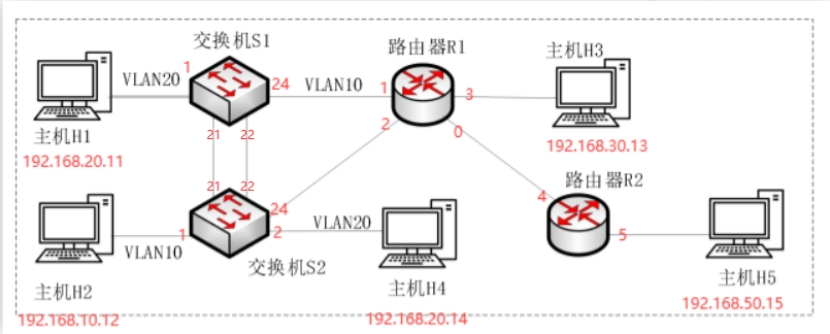
\includegraphics[width=\textwidth]{images/1.jpg}
    \caption{期末综合实验网络拓扑图}
\end{figure}

\begin{itemize}
    \item \textbf{设备使用规划:}
    使用17组和15组设备进行本次实验
    \begin{itemize}
        \item H1: 17组PC1
        \item H2: 17组PC2
        \item H3: 17组PC3
        \item H4: 15组PC2
        \item H5: 15组PC3
        \item S1: 17组交换机1(172.16.17.201)
        \item S2: 17组交换机2(172.16.17.202)
        \item R1: 17组路由器1(172.16.17.203)
        \item R2: 17组路由器2(172.16.17.204)
    \end{itemize}
    \item \textbf{物理接线:}
    
    PC <-> 交换机/路由器
    \begin{itemize}
        \item H1(PC) $\leftrightarrow$ S1 GE0/0/1
        \item H2(PC) $\leftrightarrow$ S2 GE0/0/1
        \item H3(PC) $\leftrightarrow$ R1 GE0/0/3
        \item H4(PC) $\leftrightarrow$ S2 GE0/0/2
        \item H5(PC) $\leftrightarrow$ R2 GE0/0/5
    \end{itemize}
    
    交换机 <-> 路由器
    \begin{itemize}
        \item S1 GE0/0/24 $\leftrightarrow$ R1 GE0/0/1
        \item S2 GE1/0/24 $\leftrightarrow$ R1 GE0/0/2
    \end{itemize}
    
    路由器之间
    \begin{itemize}
        \item R1 GE0/0/0 $\leftrightarrow$ R2 GE0/0/4
    \end{itemize}
    
    交换机之间
    \begin{itemize}
        \item S1 GE0/0/22 $\leftrightarrow$ S2 GE1/0/22 (RSTP 初始链路)
        \item \textit{S1 GE0/0/21 与 S2 GE1/0/21 端口为 RSTP 任务预留，暂不连接}
    \end{itemize}
    
    \item \textbf{IP 规划:}
    \begin{itemize}
        \item \textbf{VLAN 10 网段:} 192.168.10.0/24
        \item \textbf{VLAN 20 网段:} 192.168.20.0/24
        \item \textbf{H3 网段:} 192.168.30.0/24
        \item \textbf{H5 网段:} 192.168.50.0/24
        \item \textbf{R1-R2 互联:} 10.1.1.0/24
        \item \textbf{主机 IP 地址分配:}
        \begin{itemize}
            \item H1 (VLAN 20): 192.168.20.11 / 网关 192.168.20.1
            \item H2 (VLAN 10): 192.168.10.12 / 网关 192.168.10.1
            \item H3: 192.168.30.13 / 网关 192.168.30.1
            \item H4 (VLAN 20): 192.168.20.14 / 网关 192.168.20.1
            \item H5: 192.168.50.15 / 网关 192.168.50.1
        \end{itemize}
        \item \textbf{网关 IP 地址分配:}
        \begin{itemize}
            \item R1 (VLAN 10 网关): 192.168.10.1
            \item R1 (VLAN 20 网关): 192.168.20.1
            \item R1 (H3 网关): 192.168.30.1
            \item R2 (H5 网关): 192.168.50.1
        \end{itemize}
    \end{itemize}
\end{itemize}

\newpage
\section{任务一：RSTP破除网络环路}

\subsection{实验要求}

设计并实现方案解决图中 S1 与 S2 之间插上两条网线后产生的网络风暴问题，最终确保网络的稳定性和可用性。

\subsection{实验步骤与结果分析}

\subsubsection{基础配置与环路准备}

\textbf{操作描述}：禁用主机 H1 和 H4 的校园网卡，并配置 IP 地址、子网掩码及默认网关，构建基础通信环境。通过 Telnet 远程登录交换机 S1 和 S2，手动关闭默认开启的 STP 功能，以模拟无环路保护的网络环境。

\begin{figure}[H]
    \centering
    
\includegraphics[width=\textwidth]{images/2.png}
    \caption{H1 (左) 与 H4 (右) 的 IP 地址配置}
\end{figure}

\begin{lstlisting}[language=bash, caption={关闭交换机 STP 功能的命令}]
system-view
undo stp enable
quit
save
\end{lstlisting}

\begin{figure}[H]
    \centering
    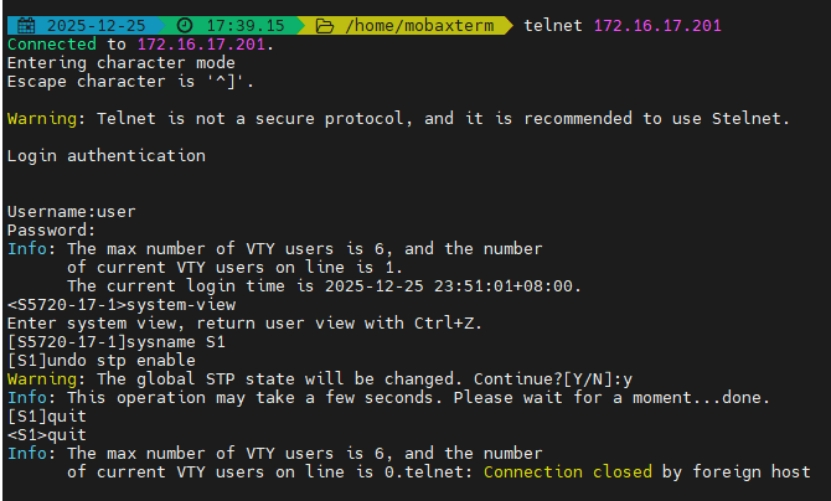
\includegraphics[width=\textwidth]{images/3.jpg}
    \caption{S1 配置过程截图}
\end{figure}

\begin{figure}[H]
    \centering
    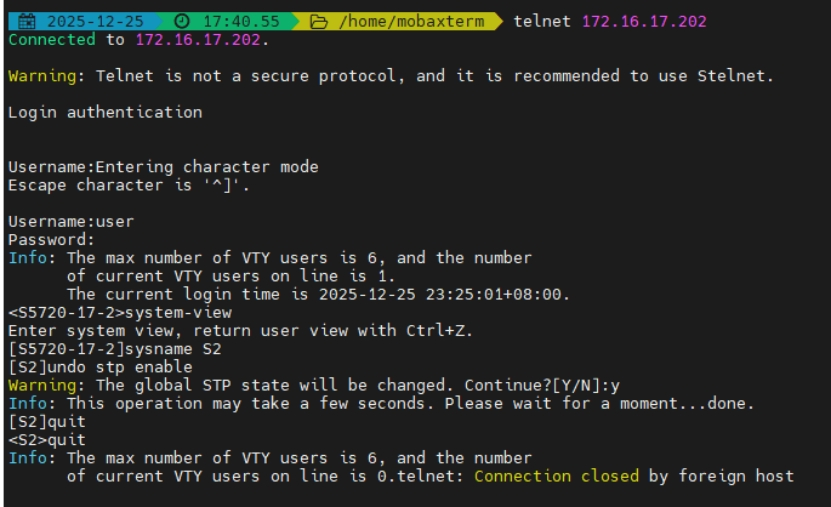
\includegraphics[width=\textwidth]{images/4.jpg}
    \caption{S2 配置过程截图}
\end{figure}

\subsubsection{基准测试：单链路通信验证}

\textbf{操作描述}：在制造环路之前，我们进行基准测试。此时 S1 与 S2 之间仅有一条物理链路（GE0/0/22 $\leftrightarrow$ GE1/0/22），网络中不存在环路。我们分别在 H1 和 H4 上执行 \texttt{ping} 命令，测试两者间的连通性。

\begin{figure}[H]
    \centering
    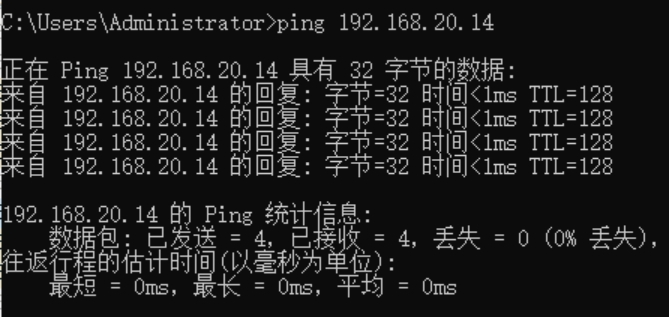
\includegraphics[width=0.7\textwidth]{images/5.jpg}
    \caption{基准测试：H1 ping H4 连通性正常}
\end{figure}

\begin{figure}[H]
    \centering
    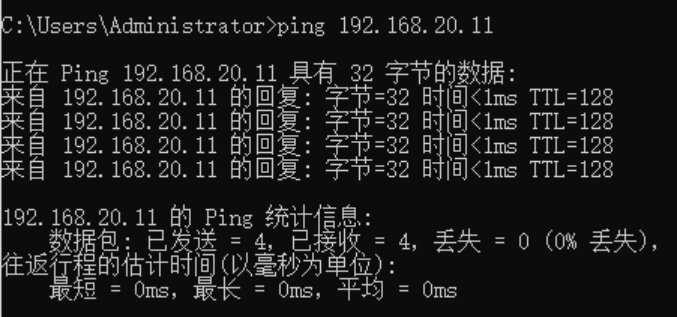
\includegraphics[width=0.7\textwidth]{images/6.jpg}
    \caption{基准测试：H4 ping H1 连通性正常}
\end{figure}

\textbf{分析}：如上图所示，在单链路的无环路环境下，H1 与 H4 之间可以正常双向通信。通过 Wireshark 抓包可以观察到标准的 ICMP Echo Request 和 Echo Reply 报文交互过程，证明了当前基础网络配置的正确性。

\begin{figure}[H]
    \centering
    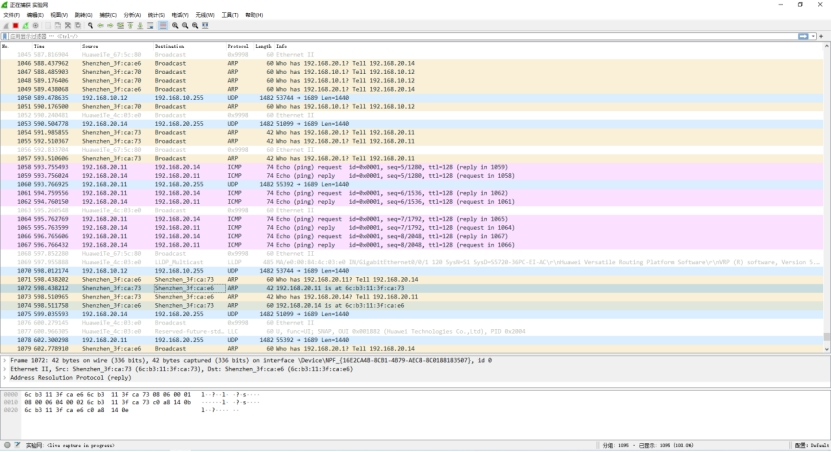
\includegraphics[width=\textwidth]{images/7.jpg}
    \caption{Wireshark 捕获 H1 ping H4 的 ICMP 流量}
\end{figure}

\begin{figure}[H]
    \centering
    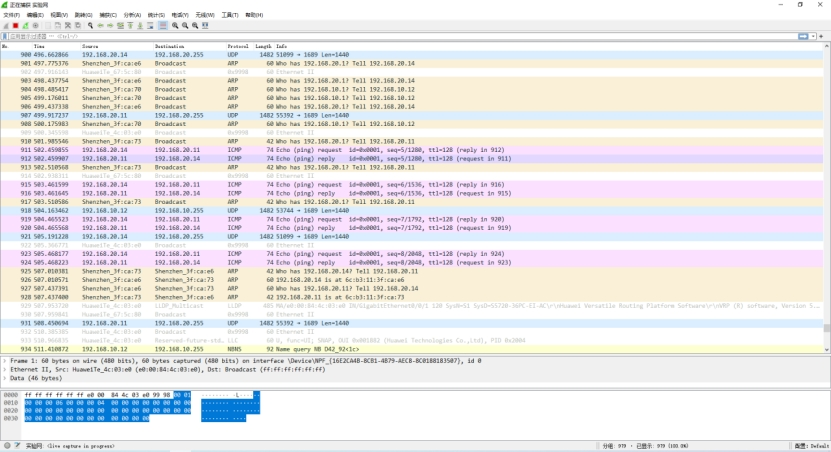
\includegraphics[width=\textwidth]{images/8.jpg}
    \caption{Wireshark 捕获 H4 ping H1 的 ICMP 流量}
\end{figure}

\subsubsection{故障模拟：制造并观察网络风暴}

\textbf{操作描述}：为了模拟故障场景，我们在 H1 上启动 Wireshark 抓包，并持续向 H4 发送 ping 请求 (\texttt{ping 192.168.20.14 -t})。在此过程中，我们手动连接 S1 与 S2 之间的第二条冗余链路 (S1 GE0/0/21 $\leftrightarrow$ S2 GE1/0/21)，从而在二层网络中制造一个物理环路。

\begin{figure}[H]
    \centering
    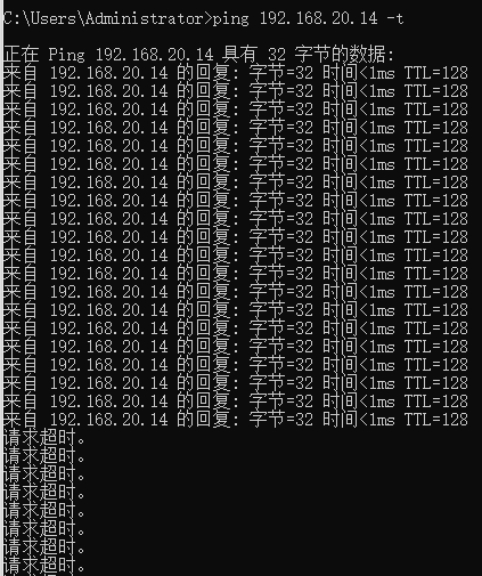
\includegraphics[width=0.7\textwidth]{images/9.jpg}
    \caption{连接第二条链路后，ping 测试迅速从正常转为“请求超时”}
\end{figure}

\textbf{状态分析}：连接第二条链路后，网络状态急剧恶化。H1 本来可以 \texttt{ping} 通但后续却无法 \texttt{ping} 通，显示“请求超时”。同时，交换机 S1 和 S2 的端口指示灯开始异常高频闪烁，表明设备正在处理大量的流量。

\begin{figure}[H]
    \centering
    
\includegraphics[width=0.7\textwidth]{images/10.png}
    \caption{网络风暴期间，交换机端口指示灯状态}
\end{figure}

Wireshark 捕获结果显示，网络中充斥着大量的 ARP 和 UDP 广播报文，短时间内捕获数据包数量达到上千万级，导致正常通信中断。这是典型的广播风暴现象：一个广播帧（如 ARP 请求）进入环路后，被两台交换机在环路链路上持续复制和转发，迅速耗尽了所有可用的网络带宽和设备处理能力，导致正常通信（如 ICMP）完全瘫痪。

\begin{figure}[H]
    \centering
    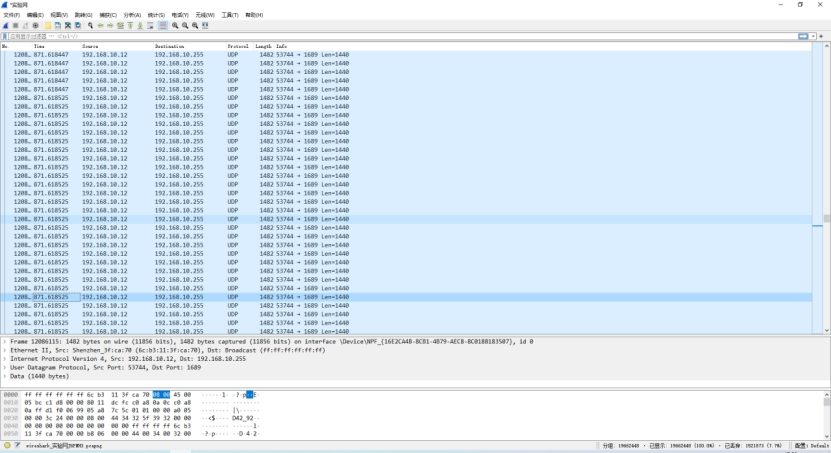
\includegraphics[width=\textwidth]{images/11.jpg}
    \caption{网络风暴中的 UDP 广播报文}
\end{figure}

\begin{figure}[H]
    \centering
    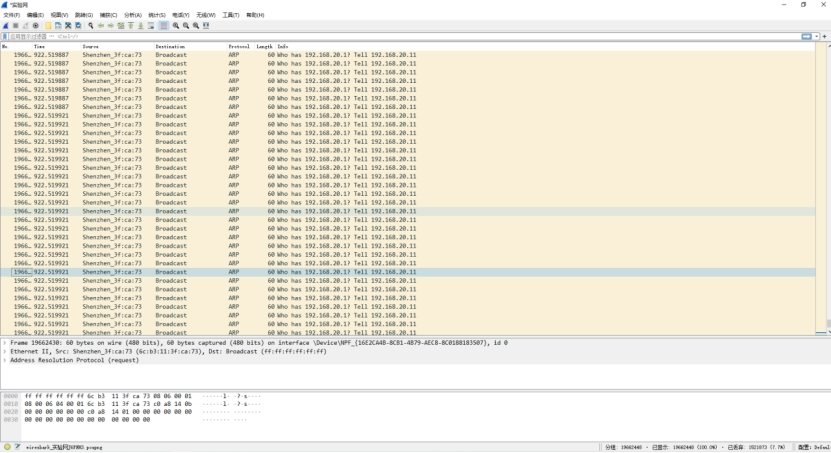
\includegraphics[width=\textwidth]{images/12.jpg}
    \caption{网络风暴中的 ARP 广播报文}
\end{figure}

\textbf{恢复操作}：观察到现象后，我们立即停止了 \texttt{ping} 命令和 Wireshark 捕获，并迅速断开新连接的 GE0/0/21 链路，以恢复网络正常。

\subsubsection{方案部署：配置RSTP并验证效果}

\textbf{操作描述}：为解决上述环路问题，我们采用快速生成树协议（RSTP）作为解决方案。RSTP 能够在逻辑上阻塞冗余链路，从而在保持物理冗余的同时，消除二层环路。我们在 S1 和 S2 上重新启用生成树功能，并将其模式设置为 \texttt{rstp}。

\begin{lstlisting}[language=bash, caption={在交换机上启用 RSTP 的命令}]
system-view
stp mode rstp
stp enable
quit
save
\end{lstlisting}

\begin{figure}[H]
    \centering
    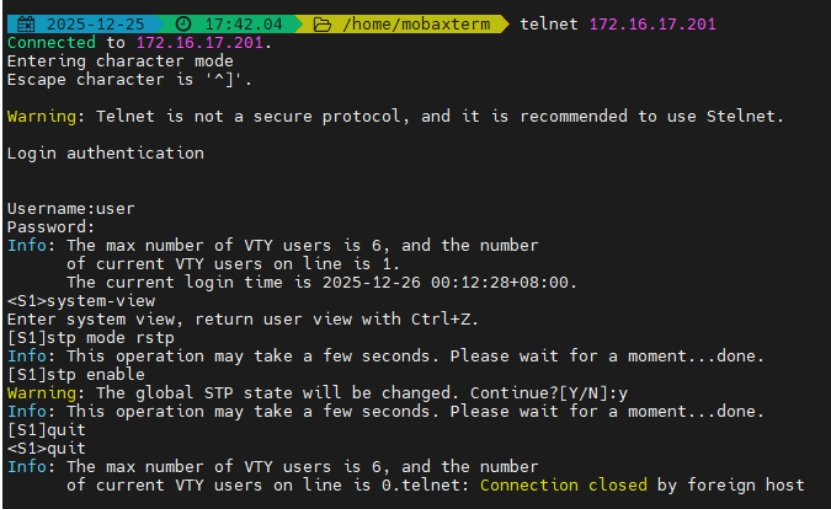
\includegraphics[width=\textwidth]{images/13.jpg}
    \caption{S1 配置过程截图}
\end{figure}

\begin{figure}[H]
    \centering
    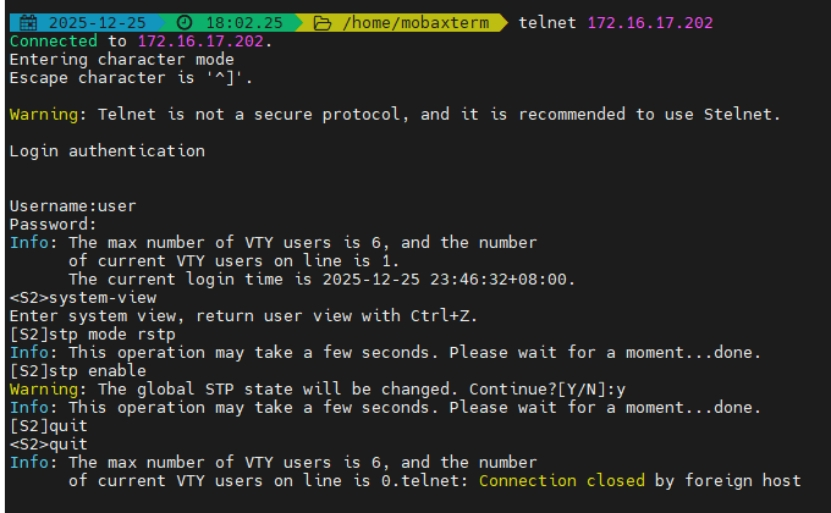
\includegraphics[width=\textwidth]{images/14.jpg}
    \caption{S2 配置过程截图}
\end{figure}

\textbf{操作描述}：配置完成后，我们再次连接 S1 与 S2 之间的两条链路，并等待约30秒以便 RSTP 协议完成收敛。随后，登录两台交换机，使用 \texttt{display stp brief} 命令查看生成树状态。

\begin{figure}[H]
    \centering
    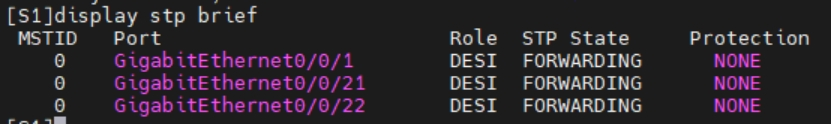
\includegraphics[width=\textwidth]{images/15.jpg}
    \caption{S1 的 \texttt{display stp brief} 命令输出}
\end{figure}

\begin{figure}[H]
    \centering
    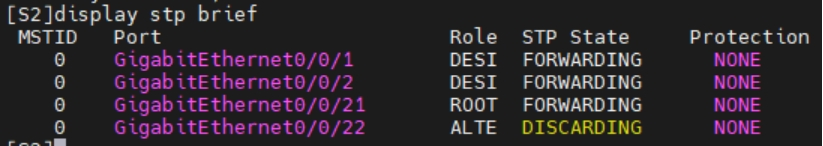
\includegraphics[width=\textwidth]{images/16.jpg}
    \caption{S2 的 \texttt{display stp brief} 命令输出}
\end{figure}

\textbf{状态分析}：\texttt{display stp brief} 的输出结果清晰地展示了 RSTP 的工作效果。在 S2 上，端口 GigabitEthernet0/0/22的角色（Role）为 \texttt{ALTE} (Alternate Port)，状态（STP State）为 \texttt{DISCARDING}。这表明 RSTP 协议成功识别出这是一个冗余端口，并将其置于阻塞状态，从而打破了物理环路，形成了一个无环的逻辑树状拓扑。而另一条链路的两端端口则处于 \texttt{FORWARDING} 状态，正常承载数据流量。

\textbf{操作描述}：在启用 RSTP 且存在两条物理链路的环境下，再次进行 H1 与 H4 之间的连通性测试。

\begin{figure}[H]
    \centering
    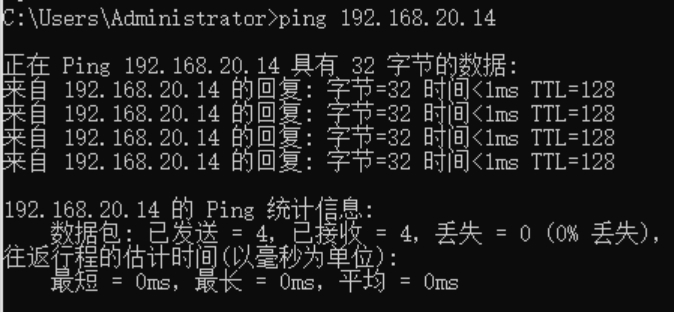
\includegraphics[width=0.75\textwidth]{images/17.jpg}
    \caption{最终验证：H1 ping H4 通信恢复正常}
\end{figure}

\begin{figure}[H]
    \centering
    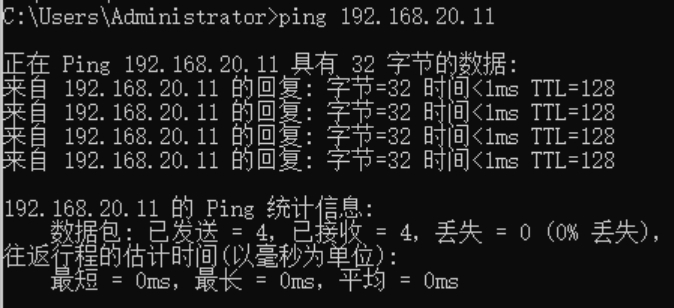
\includegraphics[width=0.75\textwidth]{images/18.jpg}
    \caption{最终验证：H4 ping H1 通信恢复正常}
\end{figure}

\textbf{分析}：测试结果表明，即使在物理上存在环路，H1 和 H4 之间的通信也完全恢复正常，网络风暴问题已得到彻底解决。

\subsection{方案总结}

\textbf{方案}：
针对交换机 S1 和 S2 之间因两条物理链路导致的网络环路问题，我们设计的解决方案是在两台交换机上全局启用并配置\textbf{快速生成树协议 (RSTP)}。RSTP 是一种二层链路管理协议，它通过在交换网络中建立一个逻辑上的无环路树状拓扑，来防止广播风暴的产生，同时提供链路冗余。当检测到网络中存在多条路径时，RSTP 会通过选举根桥和指定端口，自动将其中一条路径上的某个端口置于阻塞（\texttt{DISCARDING}）状态，从而在逻辑上断开环路。

\textbf{结果}：
实验结果验证了方案的有效性。未启用 RSTP 时，连接第二条链路引发了广播风暴。部署 RSTP 后，\texttt{display stp brief} 命令显示 S2 的 GE1/0/22 端口被置为 \texttt{DISCARDING} 状态，成功消除了环路。最终的连通性测试表明，主机间通信恢复正常，网络运行稳定。

\newpage
\section{任务二：VLAN划分与VLAN间路由}

\subsection{实验要求}

本实验要求在已有的拓扑上，通过配置 VLAN 技术实现网络的逻辑隔离与互通。具体目标为：

\begin{enumerate}
    \item 将主机 H1、H4 划入 VLAN 20，主机 H2 划入 VLAN 10。
    \item 确保同一 VLAN 内的主机（H1 与 H4）能够直接通信。
    \item 通过在路由器 R1 上配置网关，实现不同 VLAN（VLAN 10 与 VLAN 20）之间的跨网段通信（不同 VLAN 要求通过路由器连通）。
\end{enumerate}

\subsection{设计思路}

为实现VLAN的划分与VLAN间路由，我们制定了一套设计方案，来对路由器R1的网关进行配置，利用拓扑结构并避免配置冲突。

\subsubsection{基础VLAN划分与Trunking}
我们在交换机 S1 和 S2 上创建实验所需的 VLAN 10 和 VLAN 20。将直连主机的端口配置为 \texttt{Access} 模式并划入对应 VLAN，实现主机与广播域的绑定。交换机之间的互联链路则配置为 \texttt{Trunk} 模式，来承载多个VLAN的流量，确保VLAN信息可以在二层网络中正确传递。

\subsubsection{核心设计：基于拓扑的网关配置策略}
这里S1的1和24以及S2的1和2是很自然的，题都标出来了，配相应的VLAN就好。但S1和S2之间的21-22这两条路没有写明，但作为交换机互联链路，应配置为Trunk模式。所以我们主要基于以下考虑来进行配置：

\begin{itemize}
    \item \textbf{S1-R1链路}：该链路被明确指定为VLAN 10。因此，最直接且规范的配置是将R1的 \textbf{GE0/0/1} 接口作为标准的三层物理接口，专门承载VLAN 10的流量。与之对应，交换机 S1 连接此接口的端口（GE0/0/24）被配置为 \texttt{Access} 模式并划入 VLAN 10。这样，R1的GE0/0/1接口便成为了VLAN 10\textbf{唯一且专用的网关}，其IP地址配置为\texttt{192.168.10.1}。
    
    \item \textbf{S2-R1链路}：该链路被明确标注为\texttt{Trunk}，但并未指定承载某个特定的VLAN。我们当时分析，单纯为了VLAN 20的路由，将S2-GE1/0/24和R1-GE0/0/2都配置为VLAN 20的\texttt{Access}端口在功能上是可行的。但是，我们认为更贴合拓扑设计意图且更具扩展性的方案是采用\textbf{单臂路由}。因此，我们选择在R1的 \textbf{GE0/0/2} 物理接口下，\textbf{创建一个逻辑子接口 GE0/0/2.20}。通过 \texttt{dot1q termination vid 20} 命令，该子接口被指定专门处理VLAN 20的流量。我们将其IP地址配置为\texttt{192.168.20.1}，使其成为VLAN 20的\textbf{唯一网关}。
\end{itemize}

\subsection{实验步骤与结果分析}

\subsubsection{初始连通性测试 (VLAN配置前)}

\textbf{操作描述}：在进行 VLAN 配置前，我们为新增主机 H2 配置静态 IP 地址并禁用校园网卡，以此作为基准。在默认的二层交换环境下（所有端口均在默认的 VLAN 1 中），对 H1、H2、H4 之间的网络连通性进行初始评估。

\begin{figure}[H]
    \centering
    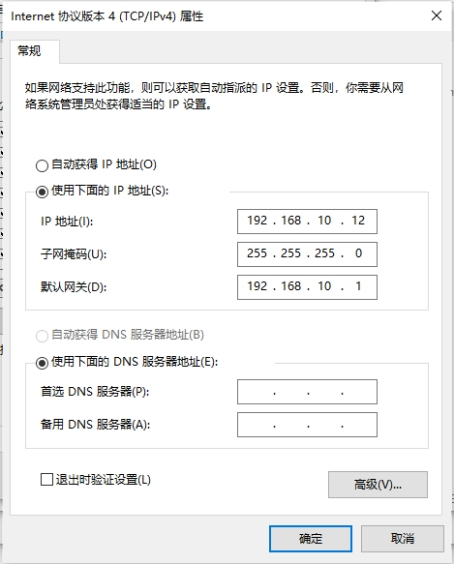
\includegraphics[width=0.45\textwidth]{images/19.jpg}
    \caption{H2 的 IP 地址配置}
\end{figure}

\textbf{测试结果与分析}：

\begin{itemize}
    \item \textbf{H1 (192.168.20.11) $\leftrightarrow$ H4 (192.168.20.14)}：\texttt{ping} 测试结果显示双向通信正常。这是因为 H1 和 H4 被规划在同一个 IP 子网中，在默认的交换环境下，它们可以通过纯二层转发自由通信。\texttt{tracert} 命令显示一跳直达，所以这是一个局域网内部的直接通信过程。

    \begin{figure}[H]
        \centering
        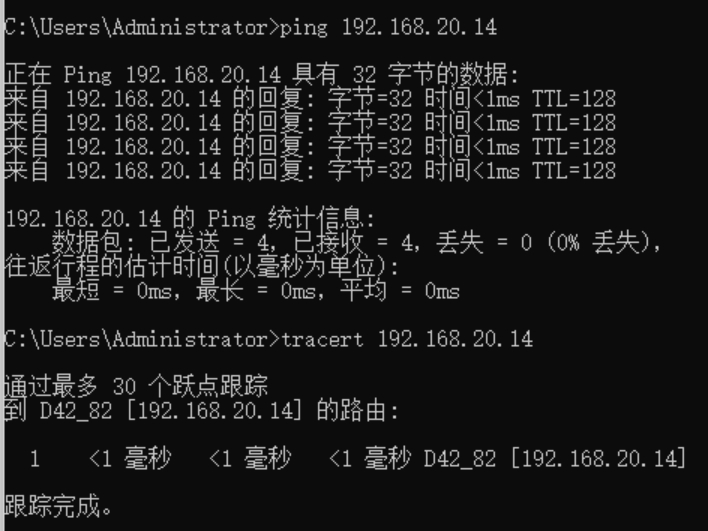
\includegraphics[width=0.7\textwidth]{images/21.jpg}
        \caption{初始状态：H1 可以 ping 通 H4}
    \end{figure}
    \begin{figure}[H]
        \centering
        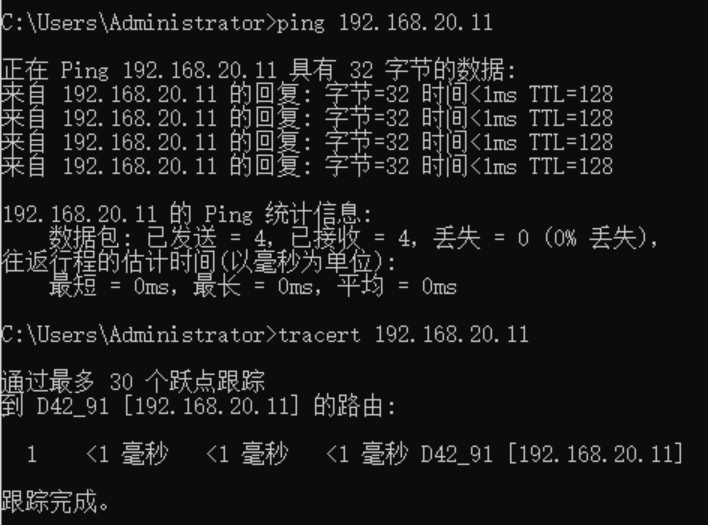
\includegraphics[width=0.7\textwidth]{images/23.jpg}
        \caption{初始状态：H4 可以 ping 通 H1}
    \end{figure}

    \item \textbf{H1/H4 $\leftrightarrow$ H2 (192.168.10.12)}：所有跨网段的 \texttt{ping} 测试均告失败。
    H1 的 ping 请求返回了来自其自身的“无法访问目标主机”的错误，这表明 H1 知道目标地址不在本地子网，但由于没有配置有效的网关，无法将数据包发送出去。
    H2 的情况类似。这个结果是符合预期的，因为它暴露了当前网络架构的局限性：缺乏一个能够连接 \texttt{192.168.10.0/24} 和 \texttt{192.168.20.0/24} 这两个独立网络的\textbf{三层路由设备}。

    \begin{figure}[H]
        \centering
        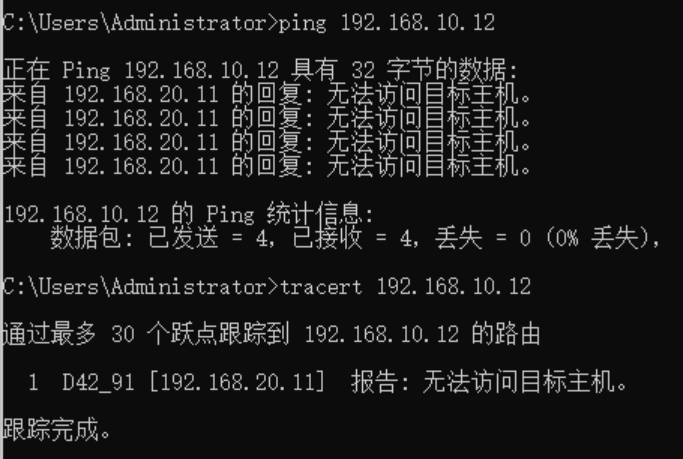
\includegraphics[width=0.7\textwidth]{images/20.jpg}
        \caption{初始状态：H1 无法 ping 通 H2}
    \end{figure}
    \begin{figure}[H]
        \centering
        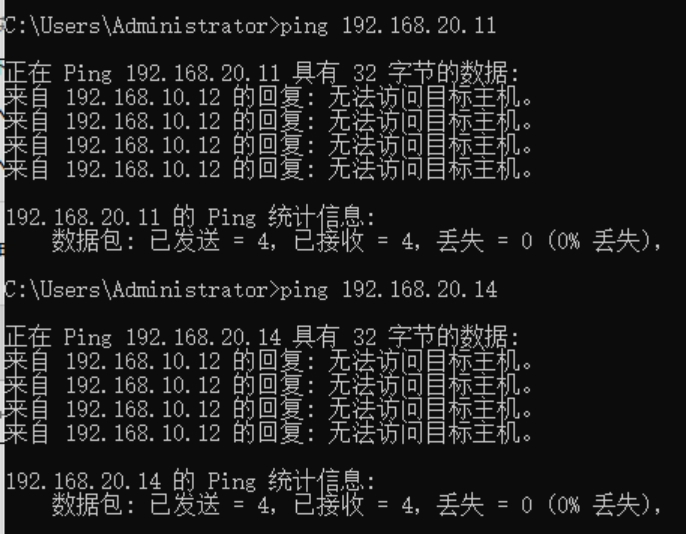
\includegraphics[width=0.7\textwidth]{images/22.jpg}
        \caption{初始状态：H2 无法 ping 通 H1 和 H4}
    \end{figure}
    \begin{figure}[H]
        \centering
        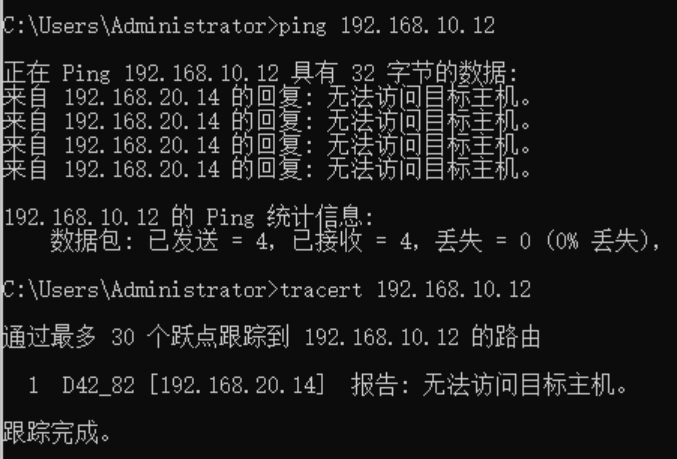
\includegraphics[width=0.7\textwidth]{images/24.jpg}
        \caption{初始状态：H4 无法 ping 通 H2}
    \end{figure}
    \end{itemize}

所以，在实现网络隔离的同时，必须构建一个可靠的三层网关来实现VLAN间的可控路由。

\subsubsection{交换机VLAN与Trunk配置}

\textbf{操作描述}：我们在交换机 S1 和 S2 上进行 VLAN 配置。具体步骤包括：批量创建 VLAN 10 和 VLAN 20；将连接主机的端口设置为 \texttt{Access} 类型并划入对应 VLAN；将设备间的互联端口配置为 \texttt{Trunk} 类型，允许所有 VLAN 流量通过。

\textbf{S1 配置命令:}

\begin{lstlisting}[language=bash, caption={交换机 S1 的 VLAN 与 Trunk 配置命令}]
system-view
! 1. 批量创建VLAN 10 和 VLAN 20
vlan batch 10 20
! 2. 配置连接H1的端口为Access模式，并划入VLAN 20
interface GigabitEthernet0/0/1
 port link-type access
 port default vlan 20
quit
! 3. 配置连接R1的端口为Access模式，并划入VLAN 10
interface GigabitEthernet0/0/24
 port link-type access
 port default vlan 10
quit
! 4. 配置连接S2的两条冗余链路为Trunk模式
interface GigabitEthernet0/0/21
 port link-type trunk
 port trunk allow-pass vlan all
quit
interface GigabitEthernet0/0/22
 port link-type trunk
 port trunk allow-pass vlan all
quit
save
\end{lstlisting}

\begin{figure}[H]
    \centering
    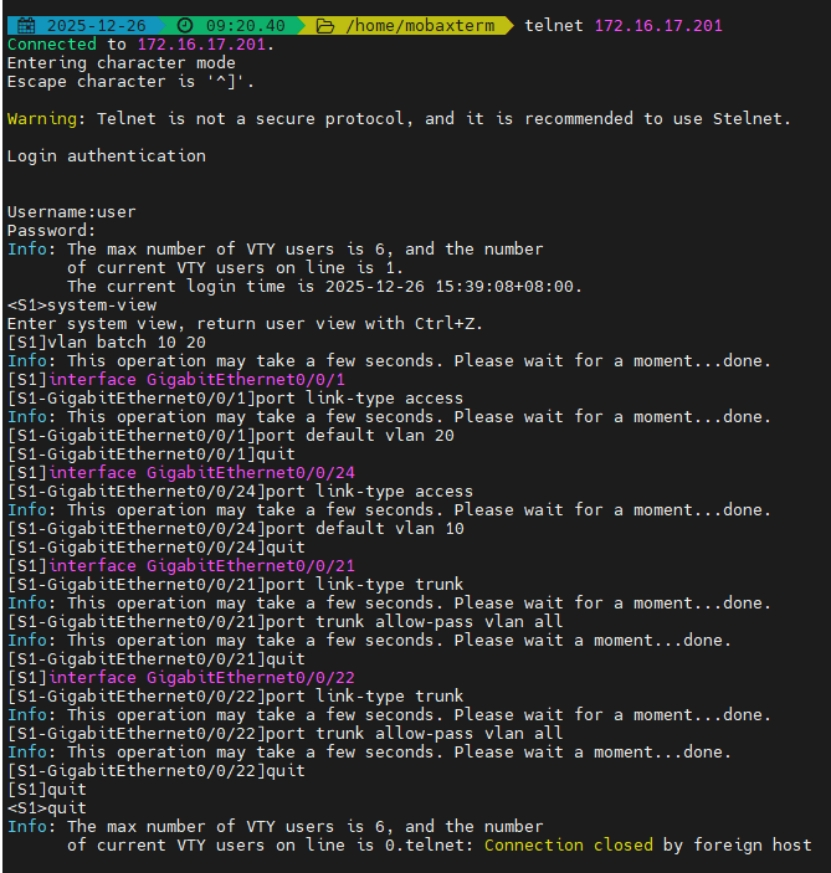
\includegraphics[width=0.9\textwidth]{images/25.jpg}
    \caption{S1 配置过程}
\end{figure}

\textbf{S2 配置命令:}

\begin{lstlisting}[language=bash, caption={交换机 S2 的 VLAN 与 Trunk 配置命令}]
system-view
! 1. 批量创建VLAN 10 和 VLAN 20
vlan batch 10 20
! 2. 配置连接H2的端口为Access模式，并划入VLAN 10
interface GigabitEthernet0/0/1
 port link-type access
 port default vlan 10
quit
! 3. 配置连接H4的端口为Access模式，并划入VLAN 20
interface GigabitEthernet0/0/2
 port link-type access
 port default vlan 20
quit
! 4. 配置连接R1的端口为Trunk模式
interface GigabitEthernet1/0/24
 port link-type trunk
 port trunk allow-pass vlan all
quit
! 5. 配置连接S1的两条冗余链路为Trunk模式
interface GigabitEthernet1/0/21
 port link-type trunk
 port trunk allow-pass vlan all
quit
interface GigabitEthernet1/0/22
 port link-type trunk
 port trunk allow-pass vlan all
quit
save
\end{lstlisting}

\begin{figure}[H]
    \centering
    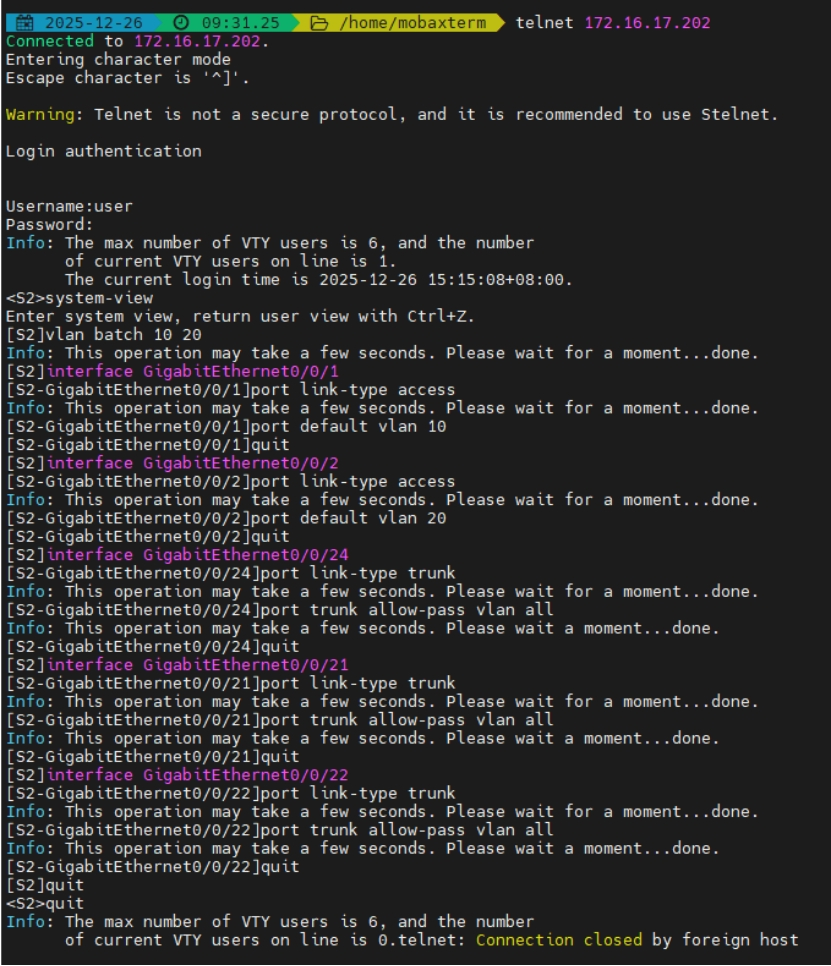
\includegraphics[width=\textwidth]{images/26.jpg}
    \caption{S2 配置过程}
\end{figure}

完成这些配置后，网络成功被划分为了 VLAN 10 和 VLAN 20这两个独立的广播域。

\subsubsection{路由器VLAN间路由配置}

\textbf{操作描述}：VLAN 间通信关键在路由器。我们登录 R1，根据预先的设计思路，配置其作为两个VLAN的网关。
我们将连接 S1 的物理接口 GE0/0/1 直接配置为 VLAN 10 的网关。
连接 S2 的 GE0/0/2，我们则启用其物理接口，并在其上创建一个绑定了VLAN 20 ID的逻辑子接口 GE0/0/2.20，将其配置为 VLAN 20 的网关。即单臂路由。

\textbf{R1 配置命令:}

\begin{lstlisting}[language=bash, caption={路由器 R1 的 VLAN 间路由配置命令}]
system-view
! --- 配置连接S1的物理接口 (VLAN 10网关) ---
interface GigabitEthernet0/0/1
 ip address 192.168.10.1 24
 undo shutdown
quit
! --- 配置连接S2的Trunk链路 ---
interface GigabitEthernet0/0/2
 undo shutdown
quit
! 创建VLAN 20的唯一网关子接口
interface GigabitEthernet0/0/2.20
 dot1q termination vid 20
 ip address 192.168.20.1 24
 arp broadcast enable
quit
save
\end{lstlisting}

\begin{figure}[H]
    \centering
    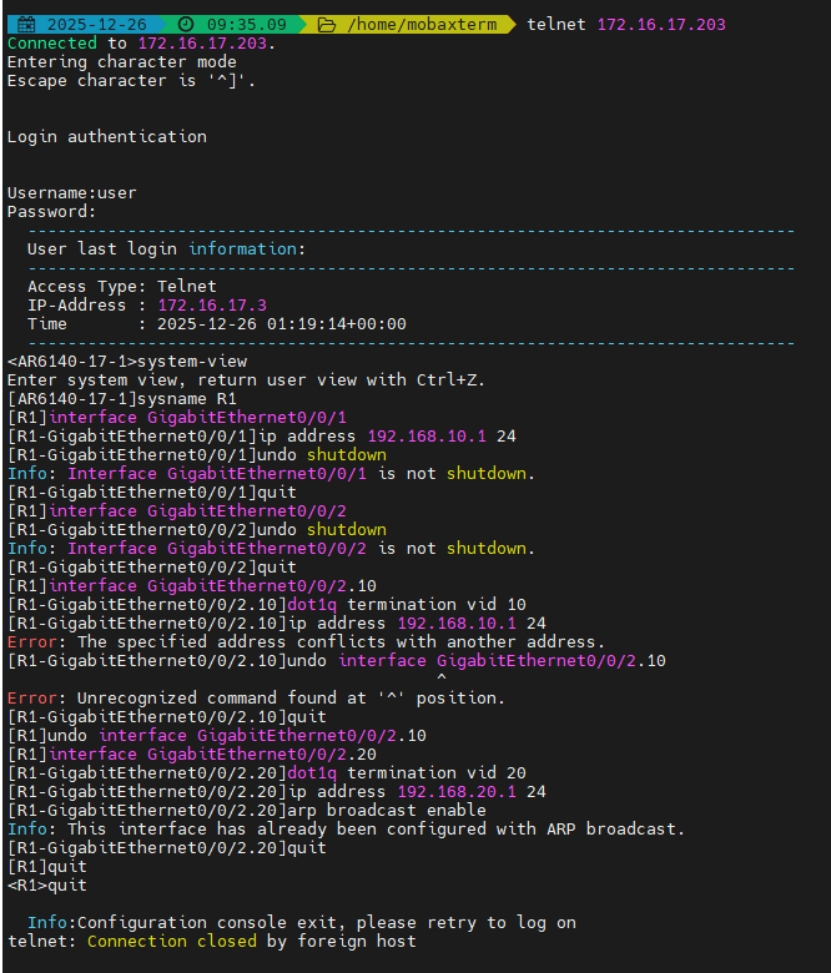
\includegraphics[width=\textwidth]{images/27.jpg}
    \caption{R1 配置过程}
\end{figure}

\textbf{配置细节分析}：在配置过程中，我们尝试为 GE0/0/2 创建另一个子接口 \texttt{.10} 并分配网关地址 \texttt{192.168.10.1}，但系统返回了地址冲突的错误。
这验证了我们的设计：GE0/0/1 物理接口已经承担了 VLAN 10 网关的职责，确保了每个VLAN网关地址的全局唯一性，从而避免了潜在的路由混乱。
此配置完成后，R1 现在拥有了两张直连路由表项，分别指向 \texttt{192.168.10.0/24} 和 \texttt{192.168.20.0/24}，具备了在这两个VLAN之间转发数据的能力。

\subsubsection{最终连通性验证 (VLAN配置后)}

\textbf{操作描述}：完成所有交换机和路由器的VLAN相关配置后，我们进行了一轮全面的连通性验证，以检验VLAN划分的隔离效果以及VLAN间路由的配置是否成功。

\textbf{测试结果与分析}:

\begin{itemize}
    \item \textbf{VLAN内通信测试 (H1 $\leftrightarrow$ H4, 均属VLAN 20)}
    \begin{itemize}
        \item \textbf{H1 ping/tracert H4}: 如图28所示，\texttt{ping}命令成功，\texttt{tracert}命令显示一跳直达目标。
        \item \textbf{H4 ping/tracert H1}: 如图29所示，结果与H1到H4的测试一致。
        \item \textbf{分析}: 这两组测试结果表明，VLAN 20内部的通信路径是畅通的。数据包在二层网络中通过交换机S1与S2之间的Trunk链路被正确转发，验证了同VLAN内的二层转发功能正常。
    \end{itemize}

    \begin{figure}[H]
        \centering
        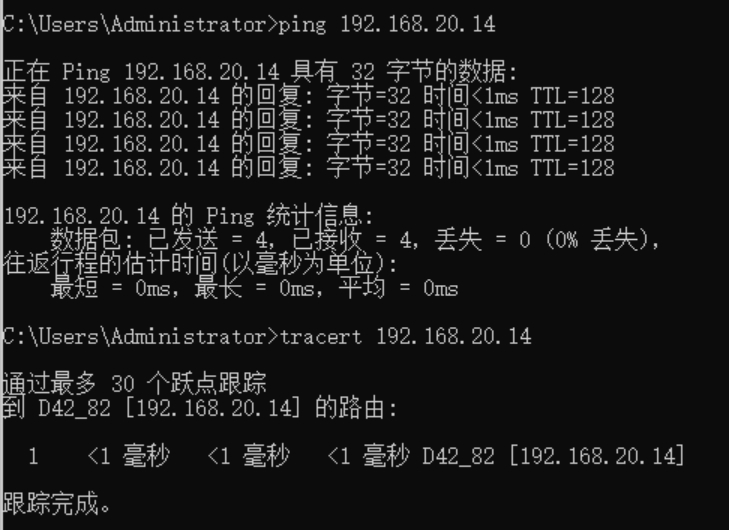
\includegraphics[width=0.7\textwidth]{images/28.jpg}
        \caption{H1 ping \& tracert H4}
    \end{figure}
    \begin{figure}[H]
        \centering
        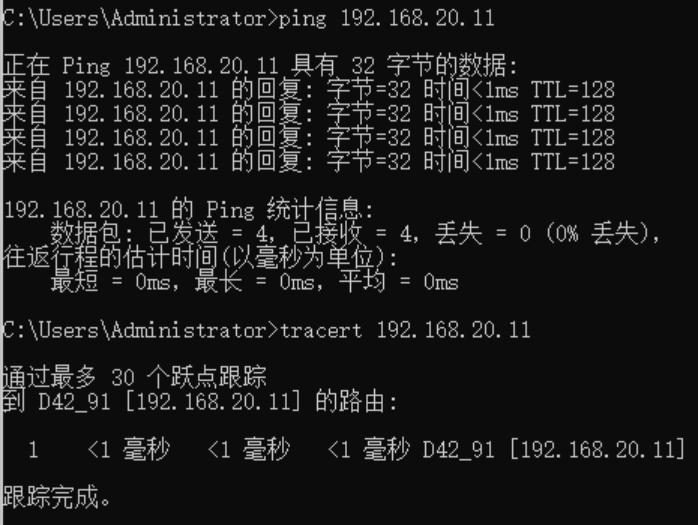
\includegraphics[width=0.7\textwidth]{images/32.jpg}
        \caption{H4 ping \& tracert H1}
    \end{figure}

    \item \textbf{VLAN间通信测试}
    \begin{itemize}
        \item \textbf{H1 (VLAN 20) $\rightarrow$ H2 (VLAN 10)}: 如图30所示，\texttt{ping}命令成功，\texttt{tracert}命令显示路径经过了两跳：第一跳为VLAN 20的网关 \texttt{192.168.20.1} (R1)，第二跳为目标主机H2。
        \item \textbf{H2 (VLAN 10) $\rightarrow$ H1 (VLAN 20)}: 如图31所示，\texttt{ping}命令成功，\texttt{tracert}命令同样显示两跳：第一跳为VLAN 10的网关 \texttt{192.168.10.1} (R1)，第二跳为目标主机H1。
        \item \textbf{H2 (VLAN 10) $\rightarrow$ H4 (VLAN 20)}: 如图32所示，\texttt{ping}与\texttt{tracert}结果与H2到H1的测试类似，验证了H2可以到达VLAN 20中的另一个成员。
        \item \textbf{H4 (VLAN 20) $\rightarrow$ H2 (VLAN 10)}: 如图33所示，\texttt{ping}与\texttt{tracert}结果与H1到H2的测试类似，验证了VLAN 20中的主机均可访问VLAN 10。
        \item \textbf{分析}: 这一系列跨VLAN的测试全部成功，表明路由器R1作为三层网关，其VLAN间路由功能已正确配置并生效。\texttt{tracert}的结果准确地反映出所有跨VLAN的数据包都必须先发送至其各自的网关地址，由路由器R1进行路由决策后，再转发至目标VLAN。
    \end{itemize}

    \begin{figure}[H]
        \centering
        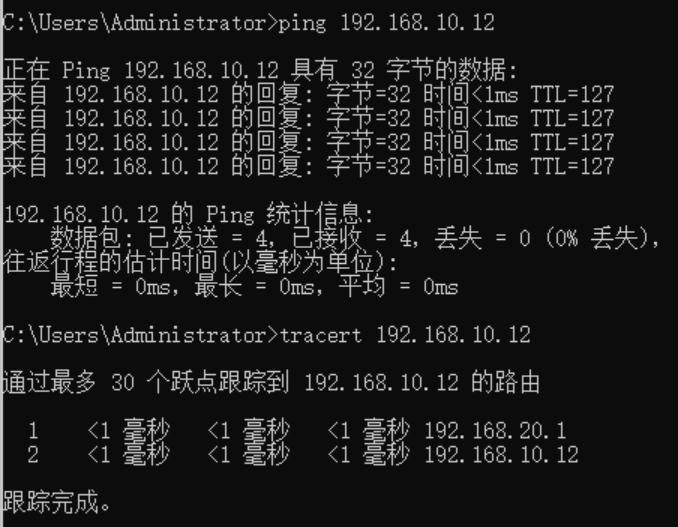
\includegraphics[width=0.7\textwidth]{images/29.jpg}
        \caption{H1 ping \& tracert H2}
    \end{figure}
    \begin{figure}[H]
        \centering
        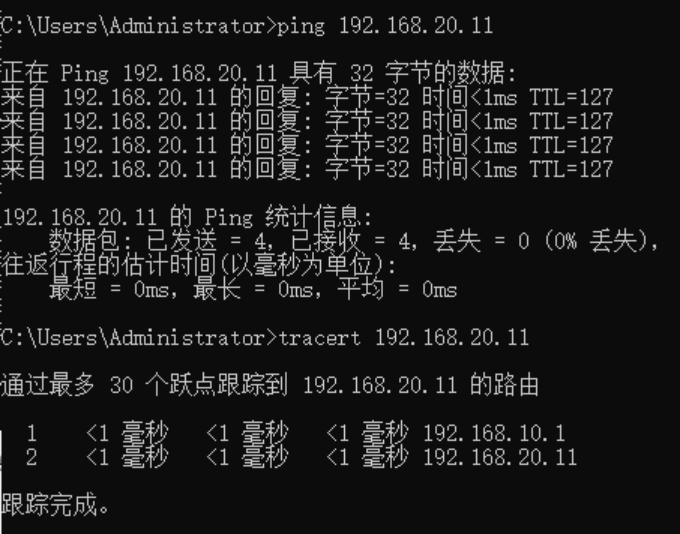
\includegraphics[width=0.7\textwidth]{images/30.jpg}
        \caption{H2 ping \& tracert H1}
    \end{figure}
    \begin{figure}[H]
        \centering
        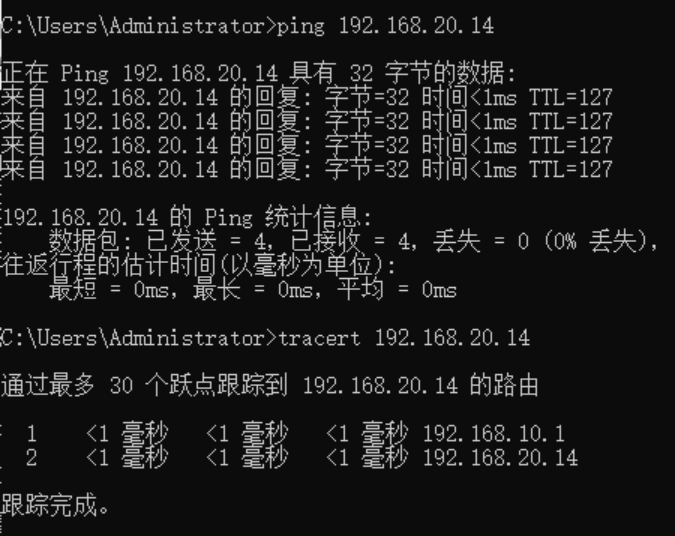
\includegraphics[width=0.7\textwidth]{images/31.jpg}
        \caption{H2 ping \& tracert H4}
    \end{figure}
    \begin{figure}[H]
        \centering
        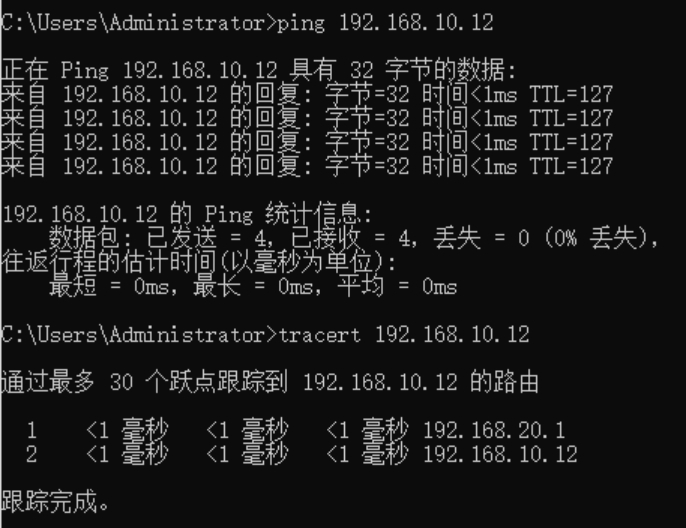
\includegraphics[width=0.7\textwidth]{images/33.jpg}
        \caption{H4 ping \& tracert H2}
    \end{figure}
\end{itemize}

综合以上所有测试，实验已成功达成任务目标：实现了VLAN的逻辑隔离，并在此基础上通过路由器实现了VLAN间的可控互通。

\subsection{路径分析}

\texttt{tracert}的结果证明了二层交换网络的透明性。
对于H1和R1等三层设备而言，S1和S2这两台交换机在数据转发过程中是不可见的。\texttt{tracert}通过IP包的TTL值来探测路由跃点，而交换机在二层转发数据帧时，并不会修改IP包头中的TTL字段。因此，无论数据帧在到达下一路由跳之前经过了多少台交换机，\texttt{tracert}都只会记录一个三层跃点。

而且，\texttt{tracert} 写出了VLAN间通信所需的三层路径模型：\textbf{主机 $\rightarrow$ 网关 (路由器) $\rightarrow$ 目标主机}。
任何跨VLAN的数据包都必须先上行至其所在VLAN的网关（路由器上的对应接口），由路由器执行路由查询，找到通往目标VLAN的路径，再将数据包下行转发到目标网络中。

\textbf{详细数据路径梳理}:
以下是本次实验中，各主机间通信的详细数据转发路径，结合了二层（L2）交换和三层（L3）路由过程：

\begin{itemize}
    \item \textbf{VLAN内通信 (H1 $\leftrightarrow$ H4)}
    \begin{itemize}
        \item \textbf{路径}: \texttt{H1 $\rightarrow$ S1 $\rightarrow$ S2 (Trunk) $\rightarrow$ H4} (H4到H1路径相反)。此为纯二层转发过程，依据MAC地址进行交换。
    \end{itemize}

    \item \textbf{VLAN间通信 (H1 $\rightarrow$ H2)}
    \begin{itemize}
        \item \textbf{路径}: \texttt{H1 $\rightarrow$ S1 $\rightarrow$ S2 (Trunk) $\rightarrow$ R1(GE0/0/2.20) $\rightarrow$ [R1内部路由] $\rightarrow$ R1(GE0/0/1) $\rightarrow$ S1 (Access) $\rightarrow$ S2 (Trunk) $\rightarrow$ H2}
    \end{itemize}

    \item \textbf{VLAN间通信 (H2 $\rightarrow$ H1)}
    \begin{itemize}
        \item \textbf{路径}: \texttt{H2 $\rightarrow$ S2 $\rightarrow$ S1 (Trunk) $\rightarrow$ R1(GE0/0/1) $\rightarrow$ [R1内部路由] $\rightarrow$ R1(GE0/0/2.20) $\rightarrow$ S2 (Trunk) $\rightarrow$ S1 (Trunk) $\rightarrow$ H1}
    \end{itemize}

    \item \textbf{VLAN间通信 (H2 $\rightarrow$ H4)}
    \begin{itemize}
        \item \textbf{路径}: \texttt{H2 $\rightarrow$ S2 $\rightarrow$ S1 (Trunk) $\rightarrow$ R1(GE0/0/1) $\rightarrow$ [R1内部路由] $\rightarrow$ R1(GE0/0/2.20) $\rightarrow$ S2 (Trunk) $\rightarrow$ H4}
    \end{itemize}

    \item \textbf{VLAN间通信 (H4 $\rightarrow$ H2)}
    \begin{itemize}
        \item \textbf{路径}: \texttt{H4 $\rightarrow$ S2 (Access) $\rightarrow$ R1(GE0/0/2.20) $\rightarrow$ [R1内部路由] $\rightarrow$ R1(GE0/0/1) $\rightarrow$ S1 (Access) $\rightarrow$ S2 (Trunk) $\rightarrow$ H2}
    \end{itemize}
\end{itemize}

通过\texttt{tracert}测试和上述路径分析，我们验证了网络分层模型中的核心概念：数据链路层（L2）负责在同一个局域网（VLAN）内进行转发，而网络层（L3）则负责在不同的网络（VLAN）之间进行寻路。

\newpage
\section{任务三：OSPF实现全网动态路由}

\subsection{实验要求}

本任务要求在 R1 与 R2 之间部署 OSPF 动态路由协议，以替代静态路由，实现全网路由信息的自动发现与收敛。最终目标是确保网络中所有主机（H1, H2, H3, H4, H5）之间都能够实现两两相互通信。

\subsection{实验流程规划}

为达成实验目标，我们规划了以下流程：

\begin{enumerate}
    \item \textbf{完成PC和路由器基础IP配置}：
    \begin{itemize}
        \item (1) 确保所有PC (H1, H2, H3, H4, H5) 的IP地址和默认网关都已按最终规划配置正确。其中，H1、H2、H4早已配好，实验开始先配好H5的（因为H3做管理机，最后再配）。
        \item (2) 确保R1和R2的所有物理接口和子接口的IP地址都已配置正确，并处于up状态。R1的GE0/0/1和GE0/0/2在实验任务1、2中已经配好，本次实验将先配好R1的GE0/0/0口和GE0/0/3口，接着配好R2的GE0/0/4口和GE0/0/5口。
    \end{itemize}

    \item \textbf{在R1上配置OSPF}：
    \begin{itemize}
        \item 启动 \texttt{ospf 1} 进程，并指定一个唯一的Router-ID (比如 1.1.1.1)。
        \item 在 \texttt{area 0} 中，使用 \texttt{network} 命令，宣告所有R1直连的业务网段（192.168.10.0, 192.168.20.0, 192.168.30.0）以及互联网络的网段（10.1.1.0）。
    \end{itemize}

    \item \textbf{在R2上配置OSPF}：
    \begin{itemize}
        \item 启动 \texttt{ospf 1} 进程，并指定另一个唯一的Router-ID (比如 2.2.2.2)。
        \item 在 \texttt{area 0} 中，也使用 \texttt{network} 命令，宣告所有R2直连的业务网段（192.168.50.0）以及互联网络的网段（10.1.1.0）。
    \end{itemize}

    \item \textbf{验证}：
    \begin{itemize}
        \item \textbf{(1) 协议层面验证}：在R1和R2上使用 \texttt{display ospf peer} 查看邻居关系是否达到 \texttt{Full} 状态。
        \item \textbf{(2) 路由层面验证}：在R1和R2上使用 \texttt{display ip routing-table} 查看是否通过OSPF学习到了对端的路由。
        \item \textbf{(3) 数据层面验证}：如果任意两台PC之间都能相互 \texttt{ping} 通，就代表全网已经连通。
    \end{itemize}
\end{enumerate}

\subsection{实验步骤与结果分析}

\subsubsection{步骤一：完成剩余设备的基础IP配置}

\textbf{操作目的}：为尚未配置IP的路由器接口（R1连接H3的接口、R2连接H5的接口、以及R1与R2之间的互联接口）分配IP地址，打通网络的三层骨架。

\textbf{分析与思考}：
在部署OSPF之前，我们必须保证OSPF邻居之间在IP层是可达的。根据我们的全局规划，我们为\textbf{R1和R2之间的互联链路（R1 GE0/0/0 $\leftrightarrow$ R2 GE0/0/4）分配了独立的网段 \texttt{10.1.1.0/24}}。R1将使用该网段的\texttt{.1}地址，R2使用\texttt{.2}地址。这条链路是OSPF交换Hello报文、建立邻居关系的通道。

\textbf{操作描述}：为 H5 主机配置静态 IP 地址，作为 R2 侧网络的测试终端。

\begin{figure}[H]
    \centering
    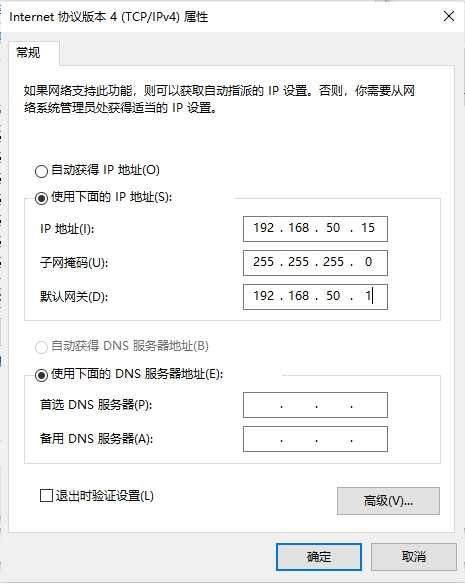
\includegraphics[width=0.6\textwidth]{images/34.jpg}
    \caption{：为H5配置IP地址 192.168.50.15，子网掩码 255.255.255.0，默认网关 192.168.50.1。}
\end{figure}

\textbf{操作描述}：接下来，我们通过Telnet远程登录R1和R2，完成所有剩余接口的IP配置。

\textbf{在R1上执行 (telnet 172.16.17.203):}

\begin{lstlisting}[language=bash, caption={：此配置为R1的GE0/0/3接口（H3的网关）和GE0/0/0接口（与R2互联）分配IP地址，并激活这些接口。}]
system-view
! 1. 配置连接H3的接口
interface GigabitEthernet0/0/3
 ! 为接口配置IP地址，作为H3的默认网关
 ip address 192.168.30.1 24
 ! 确保接口处于开启状态
 undo shutdown
quit
! 2. 配置连接R2的接口
interface GigabitEthernet0/0/0
 ! 为R1-R2互联链路配置R1侧的IP地址
 ip address 10.1.1.1 24
 undo shutdown
quit
save
\end{lstlisting}

\begin{figure}[H]
    \centering
    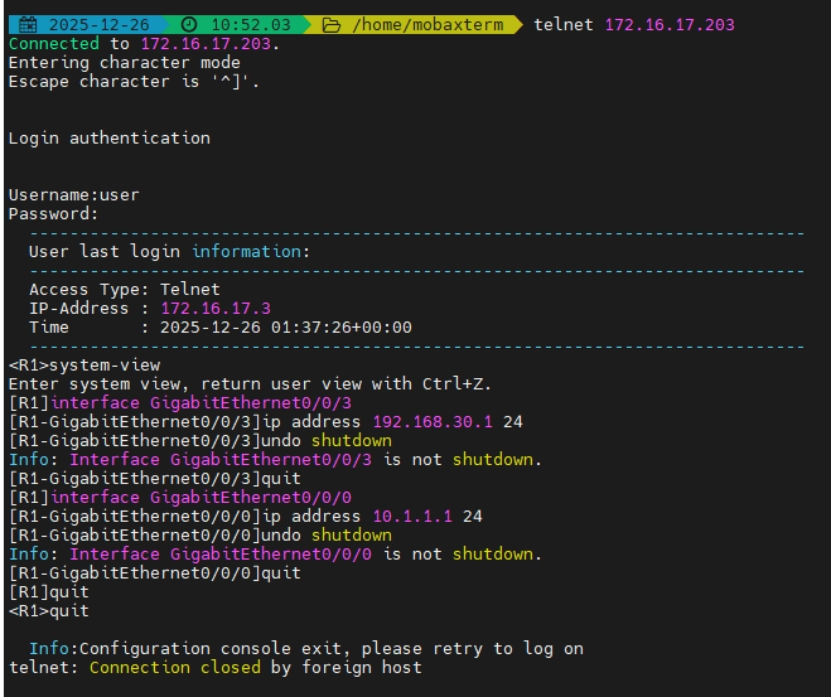
\includegraphics[width=0.8\textwidth]{images/35.jpg}
    \caption{：R1配置过程截图，显示了IP地址的成功应用和接口的激活状态。}
\end{figure}

\textbf{在R2上执行 (telnet 172.16.17.204):}

\begin{lstlisting}[language=bash, caption={：此配置为R2的GE0/0/5接口（H5的网关）和GE0/0/4接口（与R1互联）分配IP地址，并将其激活。}]
system-view
! 1. 配置连接H5的接口
interface GigabitEthernet0/0/5
 ! 为接口配置IP地址，作为H5的默认网关
 ip address 192.168.50.1 24
 undo shutdown
quit
! 2. 配置连接R1的接口
interface GigabitEthernet0/0/4
 ! 为R1-R2互联链路配置R2侧的IP地址
 ip address 10.1.1.2 24
 undo shutdown
quit
save
\end{lstlisting}

\begin{figure}[H]
    \centering
    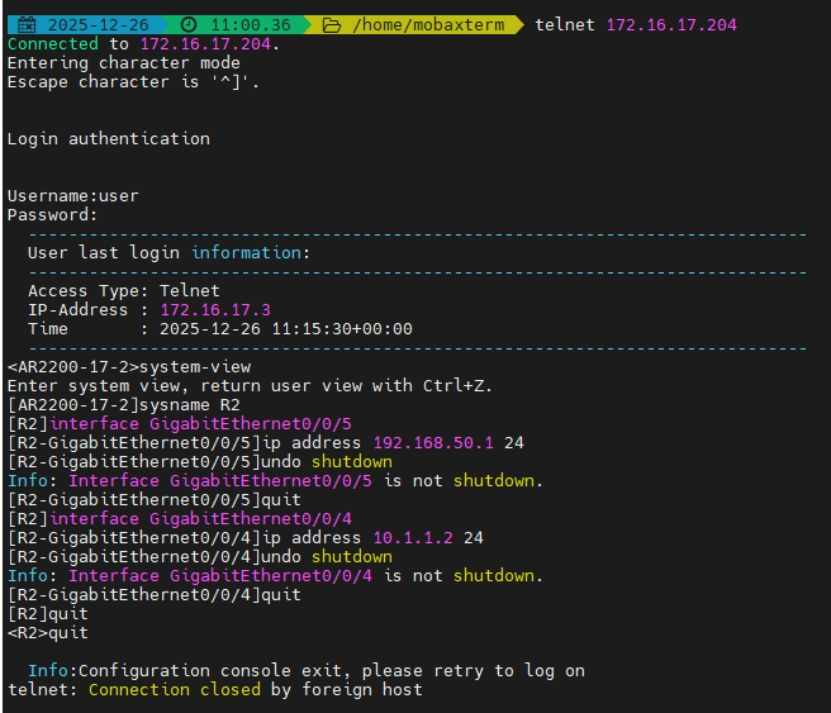
\includegraphics[width=0.8\textwidth]{images/36.jpg}
    \caption{：R2配置过程截图，确认了IP配置的正确执行。}
\end{figure}

至此，全网所有设备都拥有了IP地址，三层网络的物理和逻辑基础已搭建完毕。

\subsubsection{步骤二：OSPF部署前连通性基准测试}

\textbf{操作描述}：在启用任何路由协议之前，我们进行一次全面的基准测试以评估当前网络的路由状况。配置完成之后，先暂时禁掉H3的校园网，配置实验网的IP地址、子网掩码、默认网关，进行初始连通性测试。

\begin{figure}[H]
    \centering
    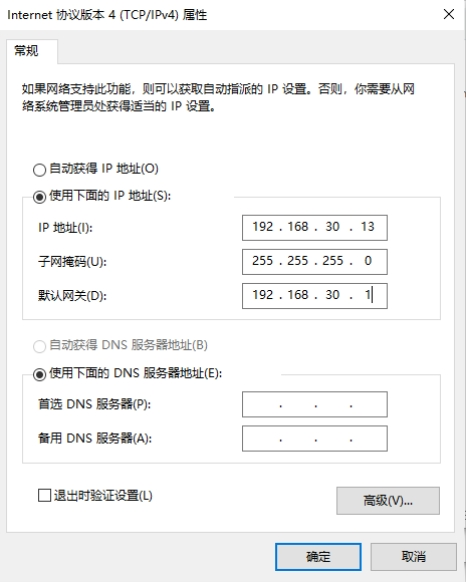
\includegraphics[width=0.7\textwidth]{images/37.jpg}
    \caption{：为作为管理主机的H3配置实验网IP，以加入连通性测试。}
\end{figure}

\textbf{测试结果与分析}：我们依次从H1、H2、H3、H4、H5 \texttt{ping} 其余四台主机。

\begin{itemize}
    \item \textbf{R1域内通信}：如图38、39、40、41所示，所有连接在R1下的主机（H1, H2, H3, H4）之间均能成功 \texttt{ping} 通。这符合预期，因为它们共享同一个网关路由器R1，R1的路由表中包含了到达这些主机所在网段的直连路由，可以在它们之间进行三层转发。
    \item \textbf{跨域通信}：所有 \texttt{ping} H5的尝试均以“请求超时”告终。反之，从H5 \texttt{ping} 其他任何主机也全部失败（如图42）。
\end{itemize}

\begin{figure}[H]
    \centering
    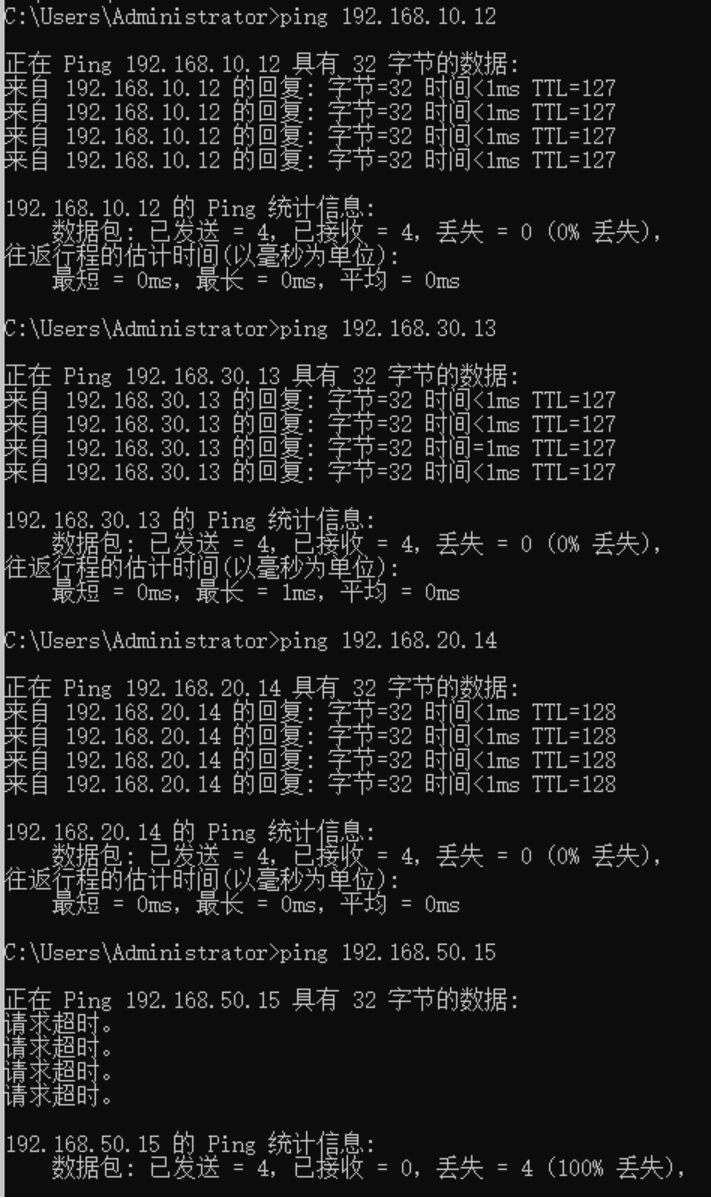
\includegraphics[width=0.8\textwidth]{images/38.jpg}
    \caption{：初始时，H1 ping其余4台主机的结果(除了H5，其余3台均能ping通)。}
\end{figure}

\begin{figure}[H]
    \centering
    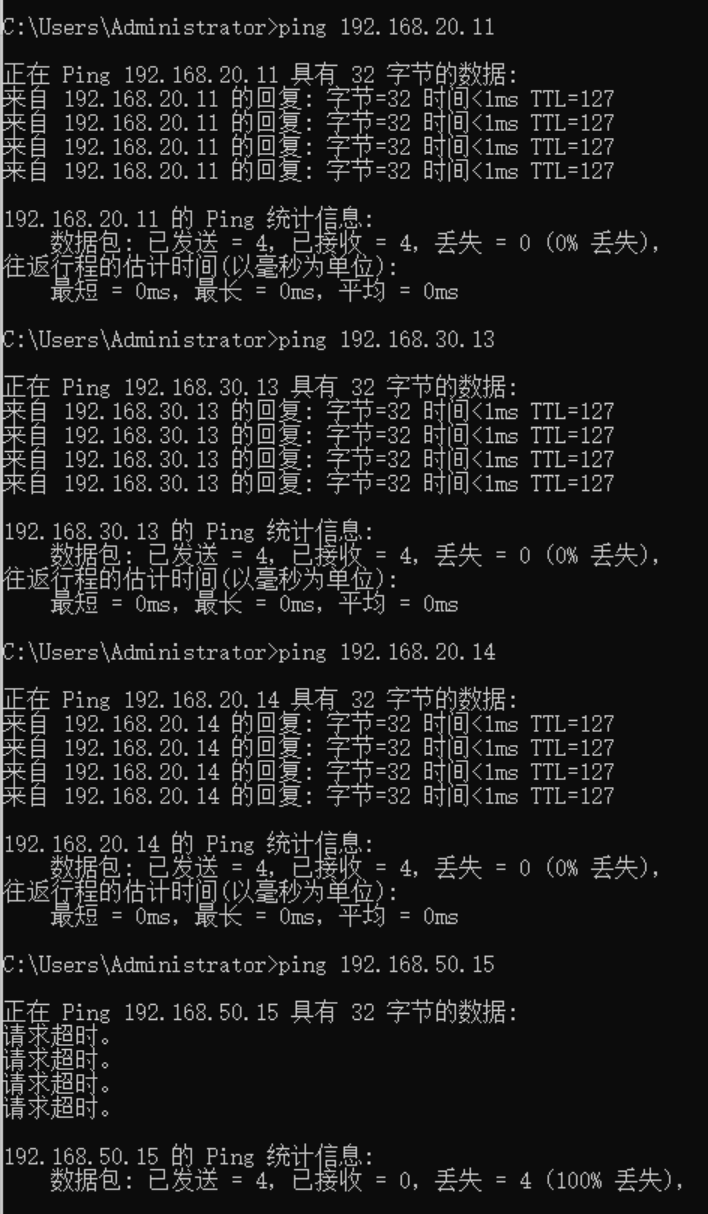
\includegraphics[width=0.8\textwidth]{images/108.png}
    \caption{：初始时，H2 ping其他4台PC的结果(除了H5，其余3台均能ping通)。}
\end{figure}

\begin{figure}[H]
    \centering
    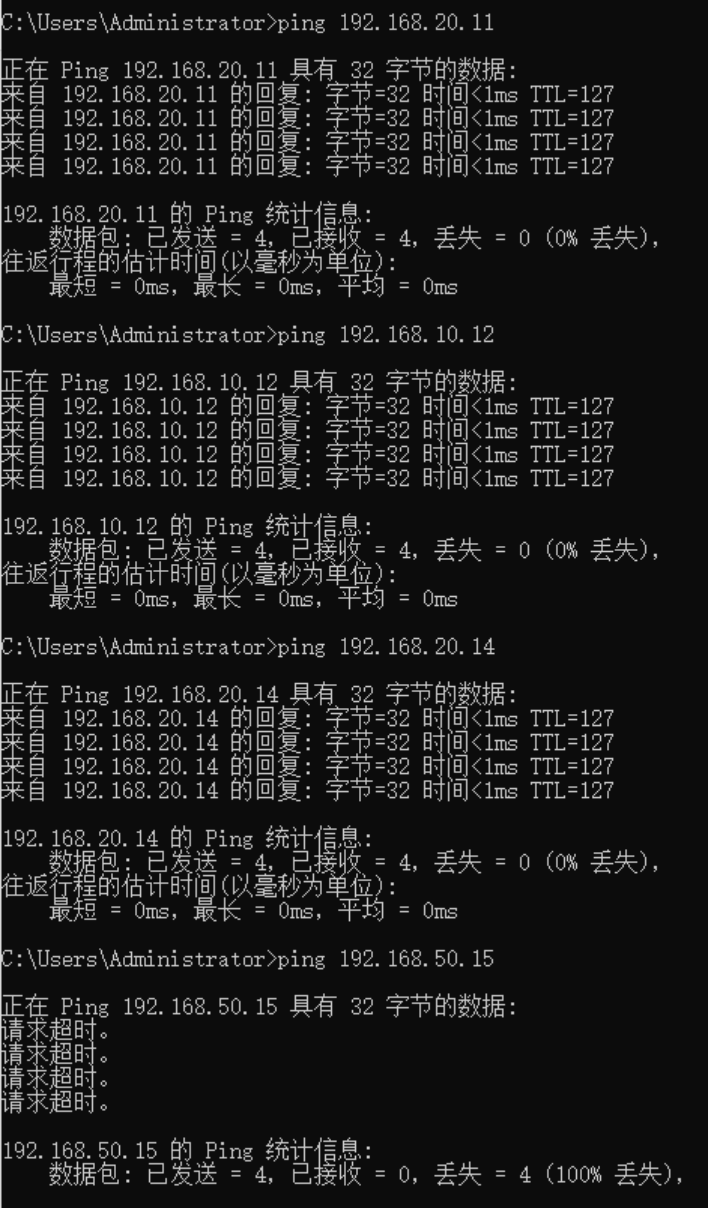
\includegraphics[width=0.8\textwidth]{images/109.png}
    \caption{：初始时，H3 ping 其余4台PC的结果(除了H5，其余3台均能ping通)。}
\end{figure}

\begin{figure}[H]
    \centering
    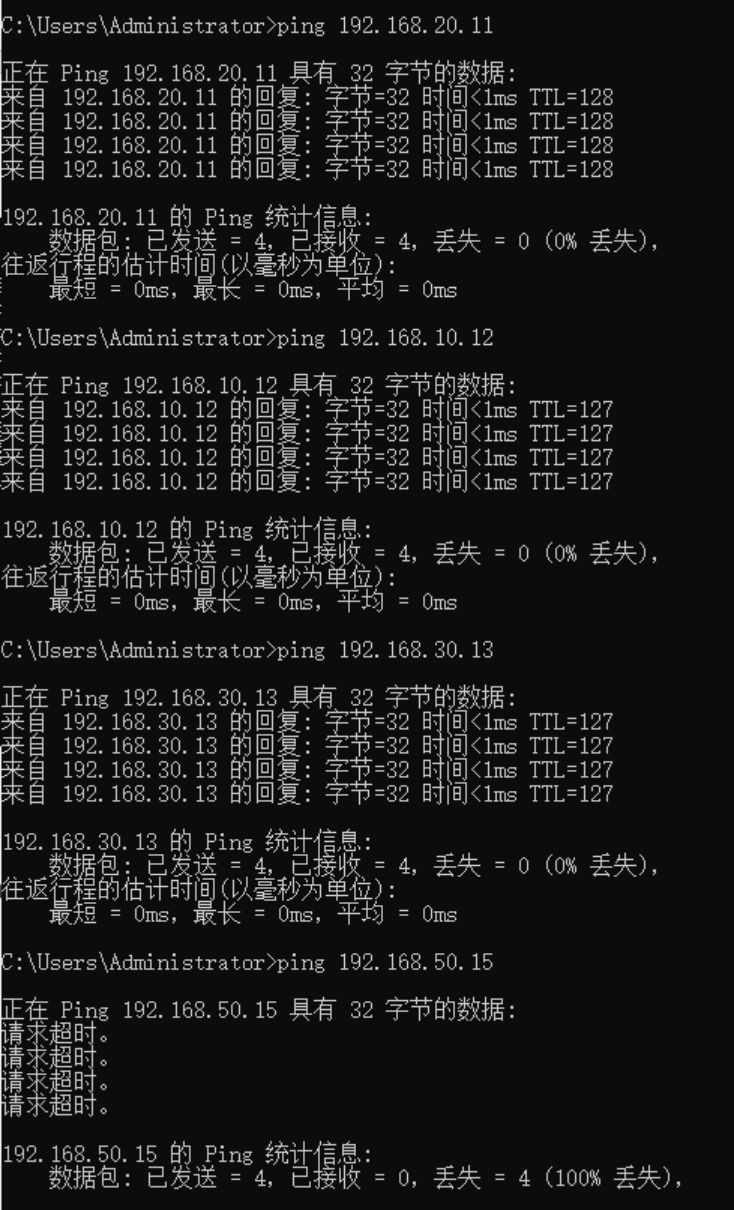
\includegraphics[width=0.8\textwidth]{images/110.png}
    \caption{：初始时，H4 ping其他4台主机的结果(除了H5，其余3台均能ping通)}
\end{figure}

\begin{figure}[H]
    \centering
    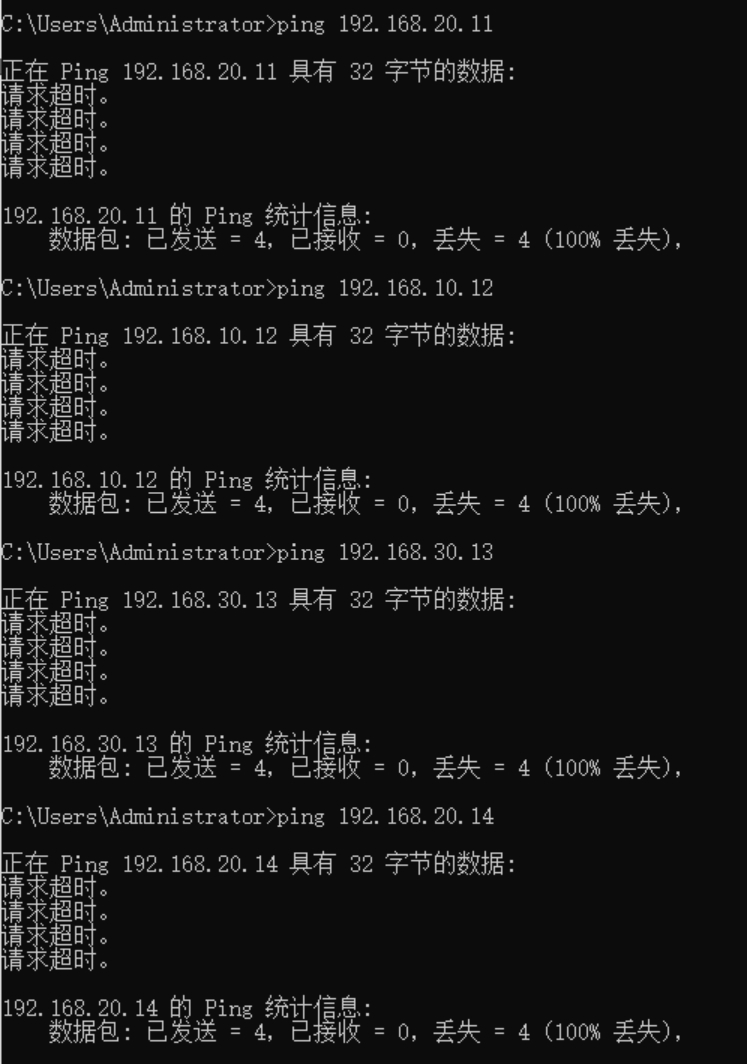
\includegraphics[width=0.8\textwidth]{images/42.jpg}
    \caption{：初始时，H5 ping不通另外的4台PC，所有数据包100\%丢失。}
\end{figure}

\textbf{原因分析}：此时由于还没有配置OSPF，R1和R2是两个隔离的路由域。R1不知道如何到达H5所在的\texttt{192.168.50.0/24}网段，同样R2也不知道如何到达R1侧的任何网段。因此，当数据包需要跨越路由器转发时，会在第一跳路由器处因“查无此路”而被丢弃。这个测试清晰地暴露了静态配置下网络的局限性，凸显了部署动态路由协议的必要性。

\subsubsection{步骤三：配置OSPF协议}

\textbf{操作目的}：在R1和R2上启动OSPF进程，并宣告所有需要被动态学习的网段，让路由器自动交换路由信息。

\textbf{操作描述}：我们重新打开H3的校园网，通过Telnet分别登录R1和R2，进行OSPF的配置。

\textbf{在R1上执行：}

\begin{lstlisting}[language=bash, caption={：在R1上启动OSPF进程，设定Router ID，并在Area 0中宣告其所有直连接口所属的网段。`network`命令的反掩码`0.0.0.255`表示精确匹配一个C类网段。}]
system-view
! 1. 启动OSPF进程1，并手动指定唯一的Router ID
ospf 1 router-id 1.1.1.1
! 2. 进入骨干区域Area 0进行配置
area 0
 ! 3. 宣告所有R1直连的业务网段
 ! 宣告VLAN 10网段
 network 192.168.10.0 0.0.0.255
 ! 宣告VLAN 20网段
 network 192.168.20.0 0.0.0.255
 ! 宣告H3所在的网段
 network 192.168.30.0 0.0.0.255
 ! 宣告与R2互联的网段
 network 10.1.1.0 0.0.0.255
quit
quit
save
\end{lstlisting}

\begin{figure}[H]
    \centering
    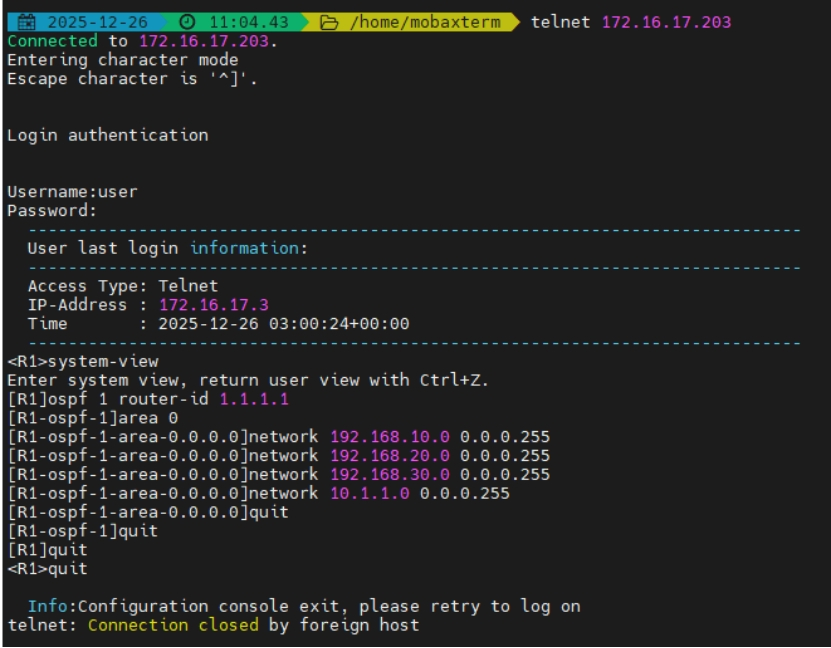
\includegraphics[width=\textwidth]{images/43.jpg}
    \caption{：R1的OSPF配置过程，所有`network`命令均被成功执行。}
\end{figure}

\textbf{在R2上执行:}

\begin{lstlisting}[language=bash, caption={：在R2上执行类似配置，宣告其直连的`192.168.50.0/24`和`10.1.1.0/24`网段，确保它能与R1建立邻居关系并交换路由。}]
system-view
! 1. 启动OSPF进程1，并指定另一个唯一的Router ID
ospf 1 router-id 2.2.2.2
! 2. 进入骨干区域Area 0
area 0
 ! 3. 宣告所有R2直连的业务网段
 ! 宣告H5所在的网段
 network 192.168.50.0 0.0.0.255
 ! 宣告与R1互联的网段
 network 10.1.1.0 0.0.0.255
quit
quit
save
\end{lstlisting}

\begin{figure}[H]
    \centering
    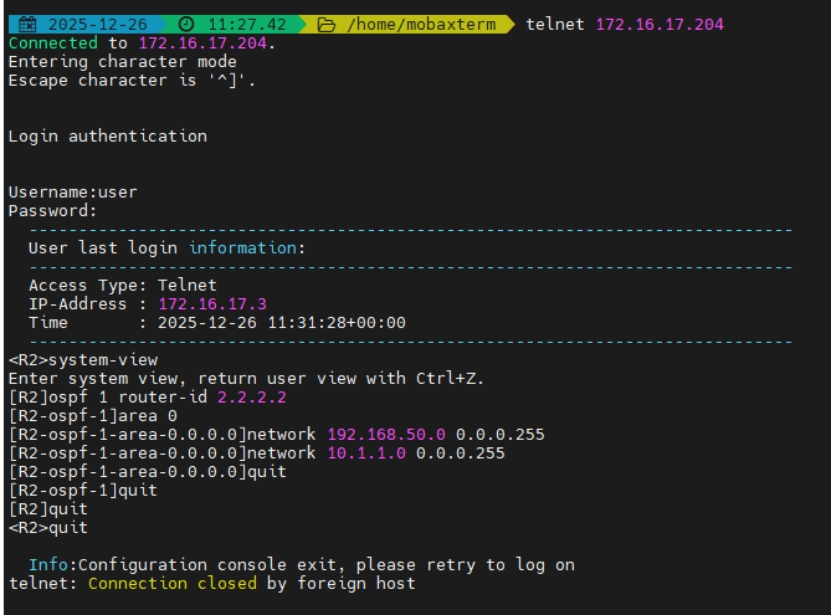
\includegraphics[width=\textwidth]{images/44.jpg}
    \caption{：R2的OSPF配置过程。}
\end{figure}

\subsubsection{步骤四：多维度验证OSPF部署效果}

\textbf{操作目的}：从协议、路由、数据三个层面，全面验证OSPF是否成功工作，网络是否已全线贯通。

\textbf{操作与验证}：稍等约40秒让OSPF收敛后，我们开始进行验证。

\textbf{协议层面验证 (查看邻居状态) + 路由层面验证 (查看路由表)}

\textbf{R1 状态检查:}
\begin{figure}[H]
    \centering
    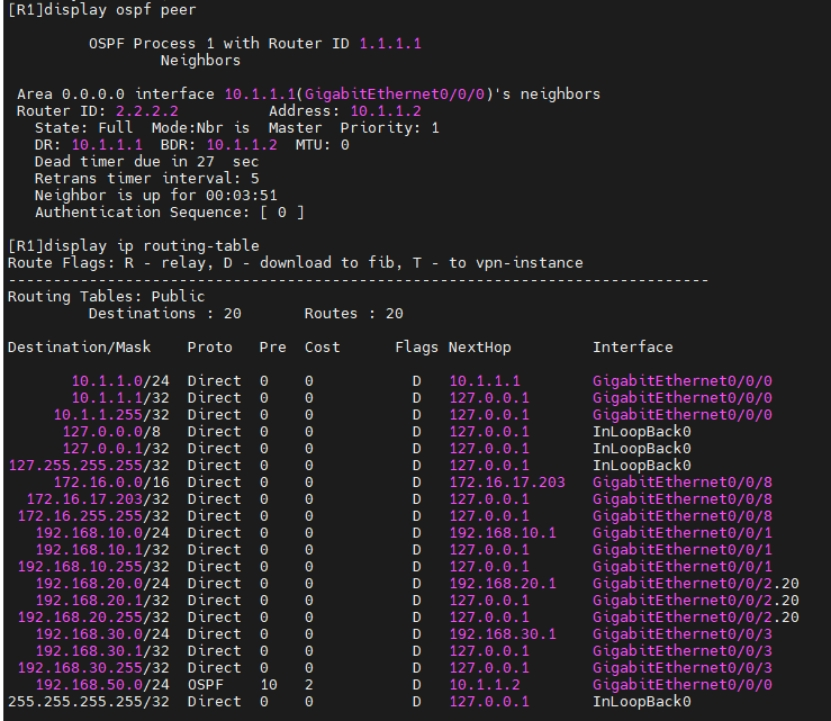
\includegraphics[width=\textwidth]{images/45.jpg}
    \caption{：在R1上执行`display ospf peer`和`display ip routing-table`的输出结果。}
\end{figure}

\textbf{分析 (R1)}：如图45所示，\texttt{display ospf peer}的输出清晰地显示了邻居R2（Router ID \texttt{2.2.2.2}）的信息，且State为 \textbf{\texttt{Full}}，这标志着两台路由器已经完成了链路状态数据库的同步，建立了最稳定的邻接关系。\texttt{display ip routing-table}的结果则提供了更有力的证据：除了直连路由，R1的路由表中新增了一条协议为 \textbf{\texttt{OSPF}} 的路由，其目的地是 \texttt{192.168.50.0/24}（H5网段），下一跳指向 \texttt{10.1.1.2}（R2的接口地址），Cost值为2。这表明R1已通过OSPF动态学习到了远程网络的可达路径。

\textbf{R2 状态检查:}
\begin{figure}[H]
    \centering
    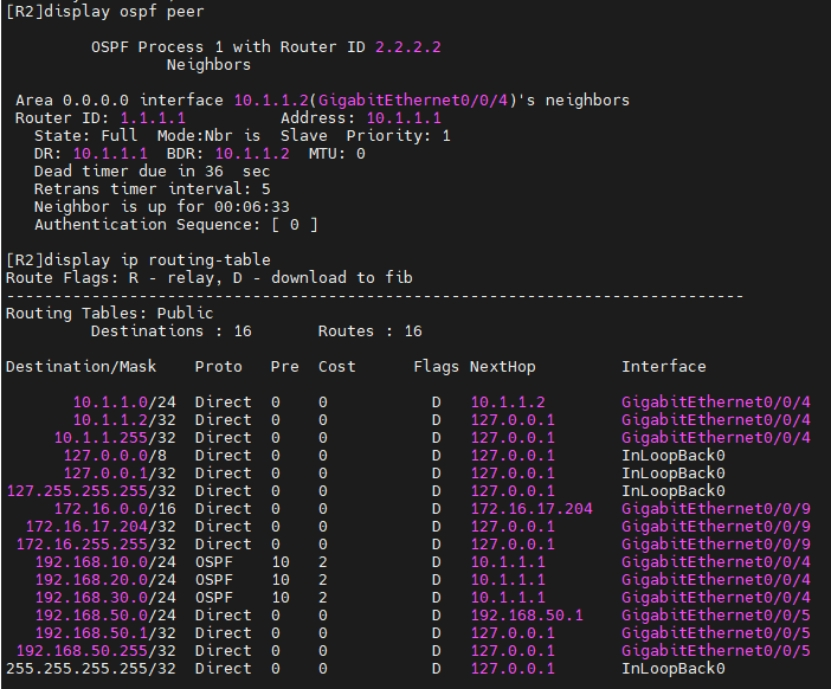
\includegraphics[width=\textwidth]{images/46.jpg}
    \caption{：在R2上执行`display ospf peer`和`display ip routing-table`的输出结果。}
\end{figure}

\textbf{分析 (R2)}：R2的检查结果符合预期。它同样与R1建立了\texttt{Full}状态的邻居关系。其路由表也通过OSPF学到了去往VLAN 10 (\texttt{192.168.10.0/24})、VLAN 20 (\texttt{192.168.20.0/24})和H3网段(\texttt{192.168.30.0/24})的多条路由，所有路由的下一跳都正确地指向了R1的地址\texttt{10.1.1.1}。

\textbf{数据层面验证 (端到端连通性)}
\textbf{操作描述}：再次进行连通性验证（重新禁掉H3的校园网卡，进行5台PC之间的连通性测试）。
\textbf{结果与分析}：现在5台PC都相互 \texttt{ping} 成功了，这表明数据包可以在全网范围内正确寻址和转发。特别是之前完全隔离的H5，现在已经可以和另外4台PC相互 \texttt{ping} 通了。这最终确认了OSPF协议已经成功地将整个网络融为一体。

\begin{figure}[H]
    \centering
    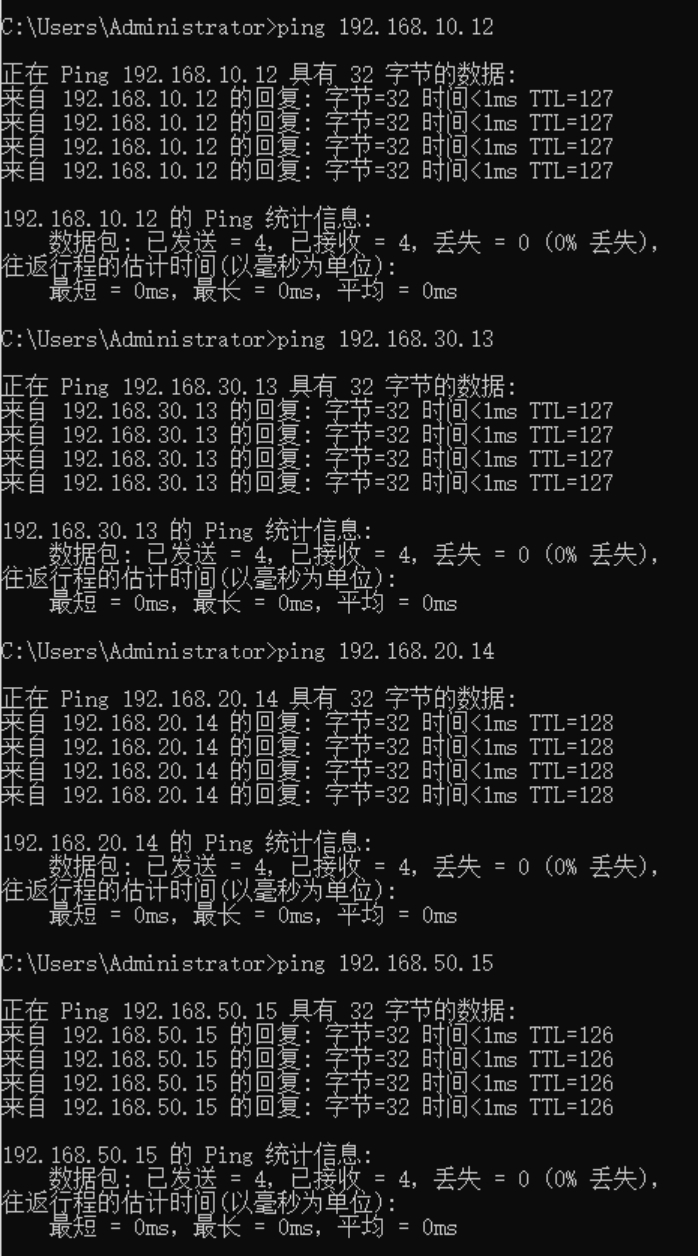
\includegraphics[width=0.8\textwidth]{images/47.jpg}
    \caption{：配置完OSPF之后，H1可以 ping通其余4台主机，包括H5。}
\end{figure}

\begin{figure}[H]
    \centering
    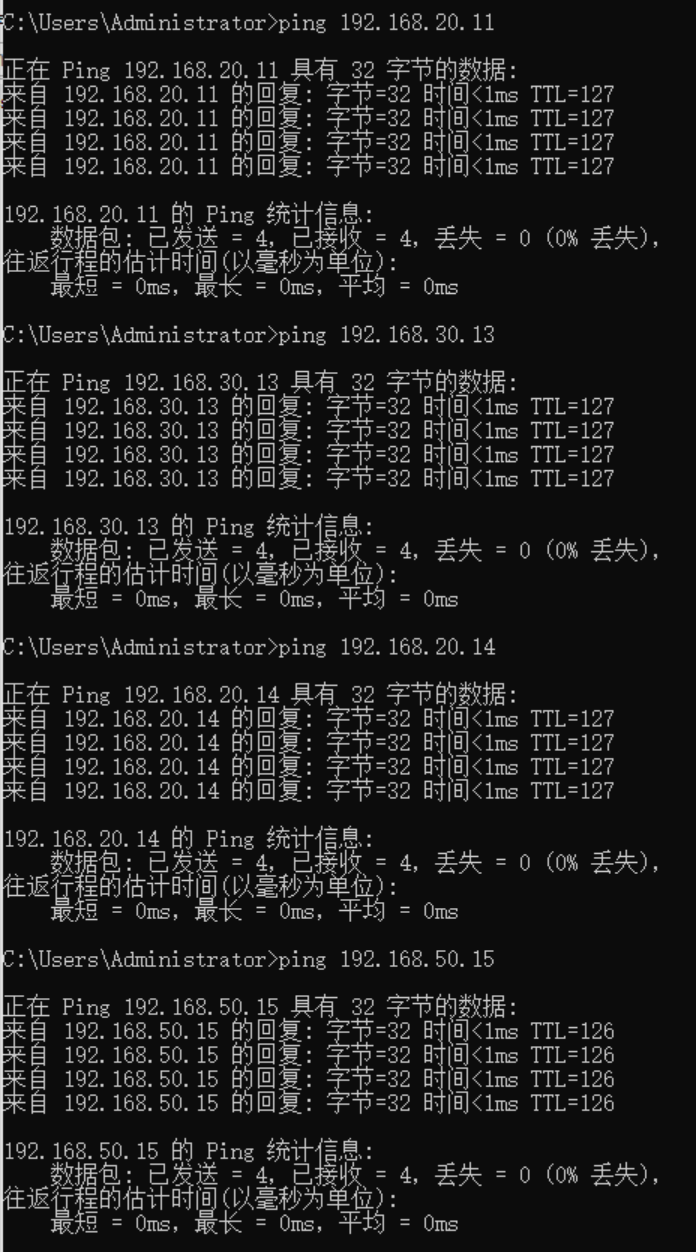
\includegraphics[width=0.8\textwidth]{images/111.png}
    \caption{：配置完OSPF之后，H2可以ping通其余4台主机。}
\end{figure}

\begin{figure}[H]
    \centering
    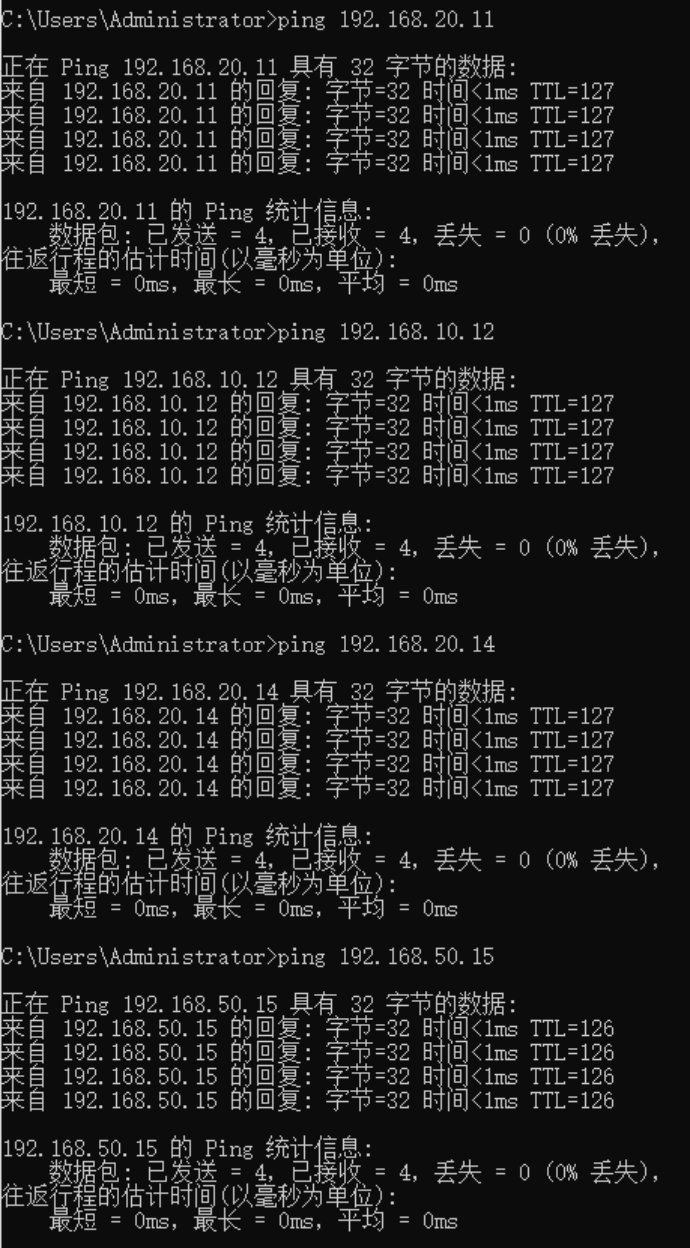
\includegraphics[width=0.8\textwidth]{images/112.png}
    \caption{：配置完OSPF之后，H3 ping其余4台PC的结果（现在连最初ping不通的H5也都可以ping通了。}
\end{figure}

\begin{figure}[H]
    \centering
    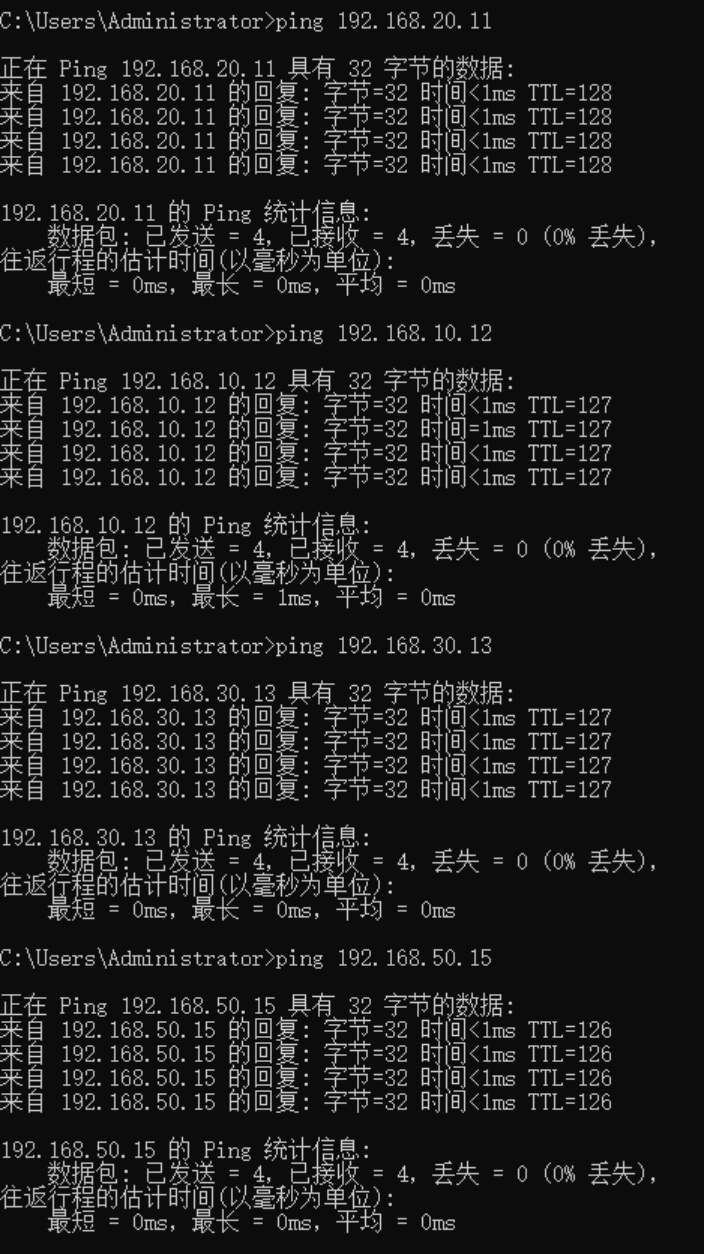
\includegraphics[width=0.8\textwidth]{images/113.png}
    \caption{：配置完OSPF之后，H4可以 ping通其他4台主机。}
\end{figure}

\begin{figure}[H]
    \centering
    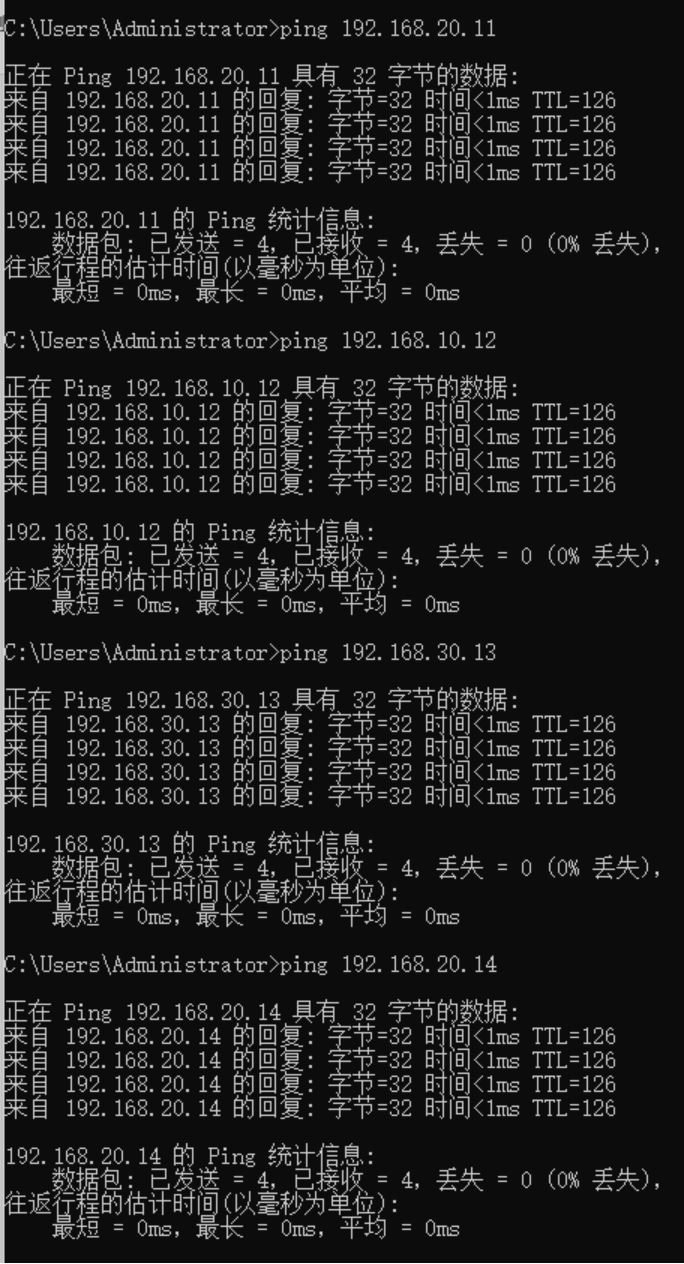
\includegraphics[width=0.8\textwidth]{images/51.jpg}
    \caption{：配置完OSPF之后，H5 可以ping通另外的4台PC。}
\end{figure}

\subsection{总结}

本次 OSPF 实验取得了预期的成功。实验初期，在仅完成基础 IP 配置而未部署任何路由协议时，我们验证了网络处于路由隔离状态：仅当主机连接至同一路由器时才能通信，跨路由器的通信则完全中断。
我们在 R1 和 R2 上启动了 OSPF 进程。使用 \texttt{network} 命令，将各个路由器直连的网段宣告进 OSPF 区域。配置完成后，通过 \texttt{display ip routing-table} 命令检查，我们观察到 R1 的路由表新增了到达 \texttt{192.168.50.0/24} 网段的 OSPF 路由，而 R2 的路由表也相应地学习到了所有 R1 侧的网段。
最终的全网连通性测试证实，所有主机之间均已能够正常 \texttt{ping} 通。实验结果表明，OSPF 协议通过自动交换路由信息，实现了网络的自动收敛与全网可达，解决了静态路由配置复杂的问题。

\newpage
\section{任务四：基于时间的复杂ACL策略部署}

\subsection{实验要求}

本实验的目标是设计并实现一套复杂的、基于时间的、双向的访问控制策略。具体要求如下：

\begin{itemize}
    \item \textbf{在 08:00\textasciitilde 11:00 时间段内}：
    \begin{itemize}
        \item H1 与 H5 可以互访，但\textbf{不允许} H1 与 H3 互通。
        \item H2 与 H3 可以互访，但\textbf{不允许} H2 与 H5 互通。
    \end{itemize}
    \item \textbf{在 14:00\textasciitilde 17:00 时间段内}：
    \begin{itemize}
        \item H1 与 H3 可以互访，但\textbf{不允许} H1 与 H5 互通。
        \item H2 与 H5 可以互访，但\textbf{不允许} H2 与 H3 互通。
    \end{itemize}
    \item \textbf{其余时段}：
    \begin{itemize}
        \item 禁止 H1 与 (H3, H5) 的互通。
        \item 禁止 H2 与 (H3, H5) 的互通。
    \end{itemize}
    \item \textbf{全局规则（不受时间限制）}：
    \begin{itemize}
        \item H1、H2 与 H4 之间的互通不受ACL限制。
        \item H3 和 H5 之间的互通不受ACL限制。
        \item H4 可以全时段自由与任意主机进行双向互通。
    \end{itemize}
\end{itemize}

\subsection{ACL设计思路与策略规划}

为满足实验要求的复杂访问控制策略，我们的整体思路是“\textbf{优先放行特权，再按时段匹配，最后全部禁止}”。

1. \textbf{策略应用点选择}：所有需要被控制的流量（H1, H2, H3, H5之间的通信）都必须经过路由器R1进行三层转发。因此，R1是应用ACL策略的最佳位置。我们将在流量进入R1的接口（GE0/0/1 和 GE0/0/2.20）的\texttt{inbound}方向应用同一套ACL，以实现对所有相关流量的集中管控。

2. \textbf{ACL规则设计原则}：
    
    设计思想为点对点、双向控制、基于时段和精细化管理。具体原则如下：
    \begin{itemize}
        \item \textbf{特权优先}：ACL规则采用自顶向下的顺序匹配，因此首先放行所有不受任何限制的“特权”流量，确保这些通信始终畅通无阻。例如，H4与全网的互通、H3与H5的互通，以及H1、H2与H4之间的互通，这些都应在ACL最前面通过\texttt{permit}规则明确允许。
        \item \textbf{上午时段（08:00--11:00）}：在该时间段内，允许H1与H5之间、H2与H3之间的双向通信，但同时严格禁止H1与H3、H2与H5之间的互通。需注意对这些主机配置\texttt{permit}和\texttt{deny}规则，且每一对主机的通信都要双向配置，确保无论谁发起连接都能被正确匹配和处理。
        \item \textbf{下午时段（14:00--17:00）}：在该时间段内，允许H1与H3、H2与H5之间的双向通信，但禁止H1与H5、H2与H3之间的互通。ACL规则需根据时间段切换\texttt{permit}和\texttt{deny}的对象，同样要保证双向配置，防止单向通信绕过限制。
        \item \textbf{其余时段}：在非上述两个时间段内，所有受控主机间（H1、H2）与（H3、H5）之间的通信进行显示禁止，实现精细化的安全策略。
    \end{itemize}

3. \textbf{规则编号与双向性}：
    \begin{itemize}
        \item \textbf{规则编号}：我们采用了更有条理的编号方式（10-39给特权，100段给上午，200段给下午，500段给全局禁止），这使得ACL更具可读性和可维护性。
        \item \textbf{双向配置}：由于\texttt{ping}等通信是双向的，ACL必须同时放行“去”和“回”两个方向的流量。因此，我们针对每一条“互通”要求，都配置了两条方向相反的\texttt{permit}规则。同样，对于“禁止互通”，我们也配置了双向的\texttt{deny}规则，确保万无一失。
    \end{itemize}

4. \textbf{ACL规则}：
    \begin{itemize}
        \item \textbf{10 \& 11}：允许H4与全网任意主机双向互通。H4作为特权主机，其通信不受任何限制，优先放行。
        \item \textbf{20 \& 21}：允许H3与H5之间双向互通。根据实验要求，H3与H5的通信全时段不受限制。
        \item \textbf{30 \& 31}：允许VLAN 10（H2）与VLAN 20（H1, H4）之间双向互访。由于H4已被10\&11规则优先放行，这里主要实现H1与H2之间的互通。
        \item \textbf{110 \& 111}：在上午时段（08:00--11:00）允许H1与H5之间双向互访。
        \item \textbf{120 \& 121}：在上午时段（08:00--11:00）允许H2与H3之间双向互访。
        \item \textbf{112 \& 113}：在上午时段（08:00--11:00）拒绝H1与H3之间的双向互访。
        \item \textbf{122 \& 123}：在上午时段（08:00--11:00）拒绝H2与H5之间的双向互访。
        \item \textbf{210 \& 211}：在下午时段（14:00--17:00）允许H1与H3之间双向互访。
        \item \textbf{220 \& 221}：在下午时段（14:00--17:00）允许H2与H5之间双向互访。
        \item \textbf{212 \& 213}：在下午时段（14:00--17:00）拒绝H1与H5之间的双向互访。
        \item \textbf{222 \& 223}：在下午时段（14:00--17:00）拒绝H2与H3之间的双向互访。
        \item \textbf{500 \& 501}：在其余所有时段禁止H1与（H3, H5）之间的双向互访。
        \item \textbf{502 \& 503}：在其余所有时段禁止H2与（H3, H5）之间的双向互访。
    \end{itemize}
    
基于以上思路，我们制定了详细的\texttt{permit}和\texttt{deny}规则清单，并将在下一步骤中具体实施。

\subsection{实验步骤与结果分析}

\subsubsection{步骤一：定义时间段 (time-range)}

\textbf{操作目的}：创建ACL规则需要绑定的时间对象。\texttt{time-range}是实现基于时间控制的前提。

\textbf{操作命令 (在R1上执行):}

\begin{lstlisting}[language=bash, caption={：创建了两个时间段对象：`morning`（上午8点到11点）和`afternoon`（下午2点到5点），`daily`参数表示该规则每天生效。}]
system-view
time-range morning 08:00 to 11:00 daily
time-range afternoon 14:00 to 17:00 daily
quit
\end{lstlisting}

\begin{figure}[H]
    \centering
    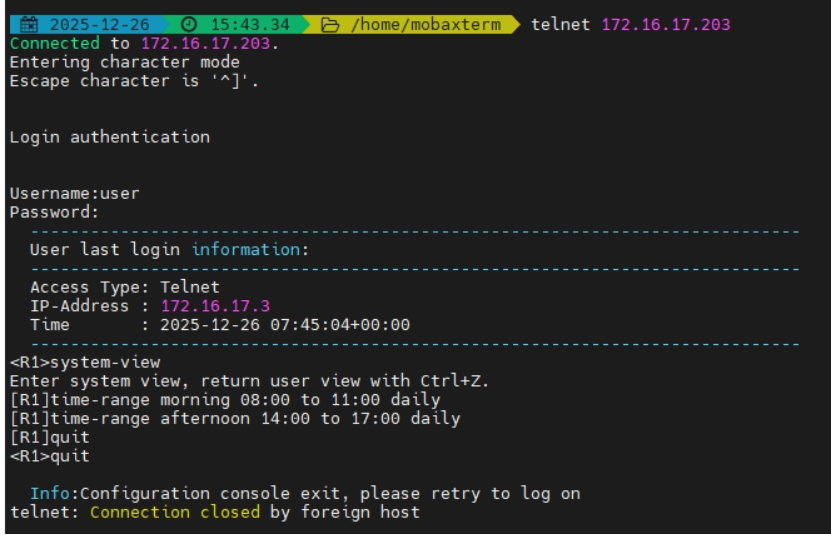
\includegraphics[width=\textwidth]{images/52.jpg}
    \caption{：R1上时间段配置过程截图，确认了`morning`和`afternoon`两个时间段的成功创建。}
\end{figure}

\subsubsection{步骤二：编写高级ACL规则 (ACL 3000)}

\textbf{操作目的}：根据我们的设计思路，在R1上创建一条高级ACL（编号3000），并写入所有\texttt{permit}和\texttt{deny}规则。

\textbf{\texttt{Permit} 规则配置 (在R1上执行):}

\begin{lstlisting}[language=bash, caption={：定义了所有的`permit`规则。注意`time-range`关键字将规则与之前定义的时间段绑定。}]
system-view
acl number 3000
! === 规则组1: 最高优先级 - 不受限的“特权”流量 ===
rule 10 permit ip source 192.168.20.14 0.0.0.0 destination any
rule 11 permit ip source any destination 192.168.20.14 0.0.0.0
rule 20 permit ip source 192.168.30.13 0.0.0.0 destination 192.168.50.15 0.0.0.0
rule 21 permit ip source 192.168.50.15 0.0.0.0 destination 192.168.30.13 0.0.0.0
rule 30 permit ip source 192.168.10.0 0.0.0.255 destination 192.168.20.0 0.0.0.255
rule 31 permit ip source 192.168.20.0 0.0.0.255 destination 192.168.10.0 0.0.0.255
! === 规则组2: 时间相关的访问策略 (精确到主机，且双向) ===
! --- 上午 (08:00 - 11:00) ---
rule 110 permit ip source 192.168.20.11 0.0.0.0 destination 192.168.50.15 0.0.0.0 time-range morning
rule 111 permit ip source 192.168.50.15 0.0.0.0 destination 192.168.20.11 0.0.0.0 time-range morning
rule 120 permit ip source 192.168.10.12 0.0.0.0 destination 192.168.30.13 0.0.0.0 time-range morning
rule 121 permit ip source 192.168.30.13 0.0.0.0 destination 192.168.10.12 0.0.0.0 time-range morning
! --- 下午 (14:00 - 17:00) ---
rule 210 permit ip source 192.168.20.11 0.0.0.0 destination 192.168.30.13 0.0.0.0 time-range afternoon
rule 211 permit ip source 192.168.30.13 0.0.0.0 destination 192.168.20.11 0.0.0.0 time-range afternoon
rule 220 permit ip source 192.168.10.12 0.0.0.0 destination 192.168.50.15 0.0.0.0 time-range afternoon
rule 221 permit ip source 192.168.50.15 0.0.0.0 destination 192.168.10.12 0.0.0.0 time-range afternoon
quit
save
\end{lstlisting}

\begin{figure}[H]
    \centering
    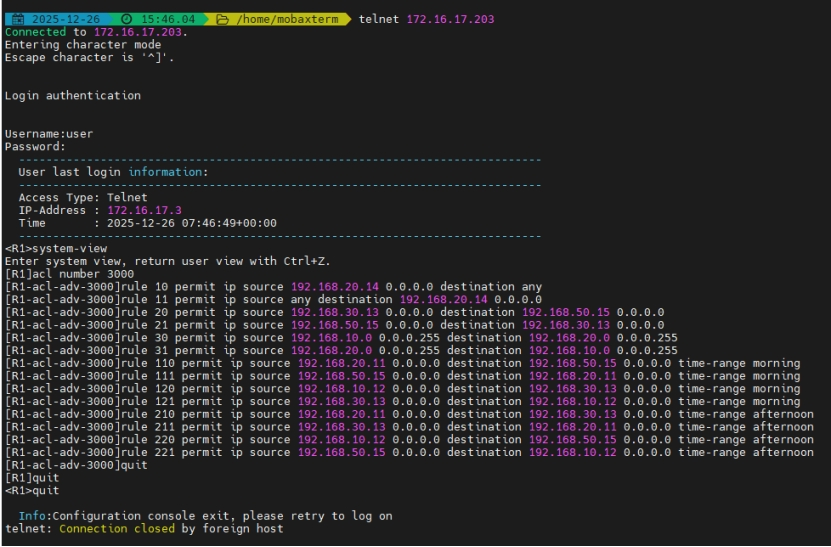
\includegraphics[width=\textwidth]{images/53.jpg}
    \caption{：在R1上编写ACL的Permit规则的配置过程。}
\end{figure}

\textbf{\texttt{Deny} 规则配置 (在R1上执行):}

\begin{lstlisting}[language=bash, caption={：定义了所有的`deny`规则。规则500-513没有绑定时间，它们的作用是捕获所有未被前面时间规则`permit`的特定流量，从而实现“其余时段”的禁止策略。}]
system-view
acl number 3000
! === 规则组2: 时间相关的访问策略 ===
! --- 上午 (08:00 - 11:00) ---
rule 112 deny ip source 192.168.20.11 0.0.0.0 destination 192.168.30.13 0.0.0.0 time-range morning
rule 113 deny ip source 192.168.30.13 0.0.0.0 destination 192.168.20.11 0.0.0.0 time-range morning
rule 122 deny ip source 192.168.10.12 0.0.0.0 destination 192.168.50.15 0.0.0.0 time-range morning
rule 123 deny ip source 192.168.50.15 0.0.0.0 destination 192.168.10.12 0.0.0.0 time-range morning
! --- 下午 (14:00 - 17:00) ---
rule 212 deny ip source 192.168.20.11 0.0.0.0 destination 192.168.50.15 0.0.0.0 time-range afternoon
rule 213 deny ip source 192.168.50.15 0.0.0.0 destination 192.168.20.11 0.0.0.0 time-range afternoon
rule 222 deny ip source 192.168.10.12 0.0.0.0 destination 192.168.30.13 0.0.0.0 time-range afternoon
rule 223 deny ip source 192.168.30.13 0.0.0.0 destination 192.168.10.12 0.0.0.0 time-range afternoon
! === 规则组3: "其余时段"的显式拒绝 ===
rule 500 deny ip source 192.168.20.11 0.0.0.0 destination 192.168.30.13 0.0.0.0
rule 501 deny ip source 192.168.20.11 0.0.0.0 destination 192.168.50.15 0.0.0.0
rule 502 deny ip source 192.168.10.12 0.0.0.0 destination 192.168.30.13 0.0.0.0
rule 503 deny ip source 192.168.10.12 0.0.0.0 destination 192.168.50.15 0.0.0.0
!  反向的deny
rule 510 deny ip source 192.168.30.13 0.0.0.0 destination 192.168.20.11 0.0.0.0
rule 511 deny ip source 192.168.50.15 0.0.0.0 destination 192.168.20.11 0.0.0.0
rule 512 deny ip source 192.168.30.13 0.0.0.0 destination 192.168.10.12 0.0.0.0
rule 513 deny ip source 192.168.50.15 0.0.0.0 destination 192.168.10.12 0.0.0.0
quit
save
\end{lstlisting}

\begin{figure}[H]
    \centering
    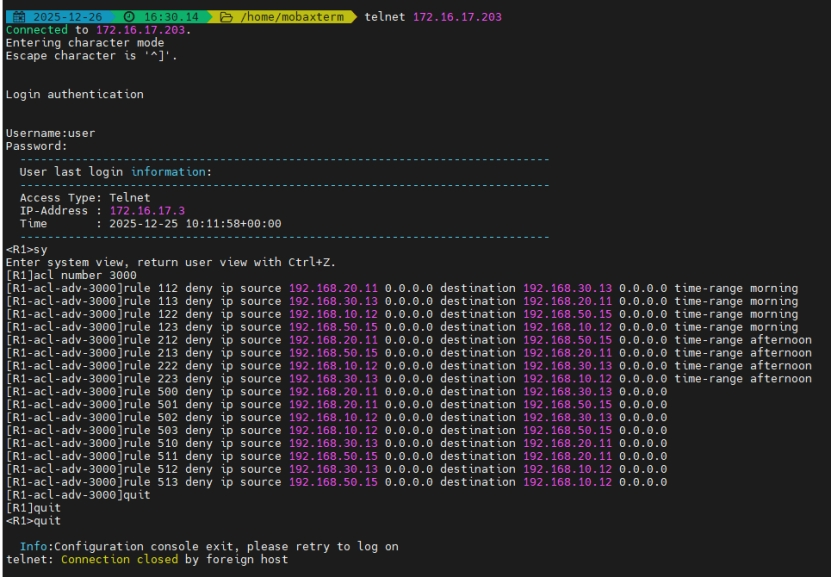
\includegraphics[width=\textwidth]{images/55.jpg}
    \caption{：在R1上编写ACL的Deny规则的配置过程。}
\end{figure}

\subsubsection{步骤三：在路由器接口应用ACL}

\textbf{操作目的}：在正确的流量入口激活ACL策略。ACL规则写好后只是“剧本”，必须应用到接口上才能“上演”。

\textbf{操作命令 (在R1上执行)：}

\begin{lstlisting}[language=bash, caption={：`traffic-filter inbound`命令将ACL 3000应用于两个网关接口的入方向。这意味着任何试图通过这两个接口进入路由器进行三层转发的数据包，都必须先经过ACL 3000的检查。}]
system-view
! 1. 应用到VLAN 10的网关接口
interface GigabitEthernet0/0/1
 traffic-filter inbound acl 3000
quit
! 2. 应用到VLAN 20的网关子接口
interface GigabitEthernet0/0/2.20
 traffic-filter inbound acl 3000
quit
save
\end{lstlisting}

\begin{figure}[H]
    \centering
    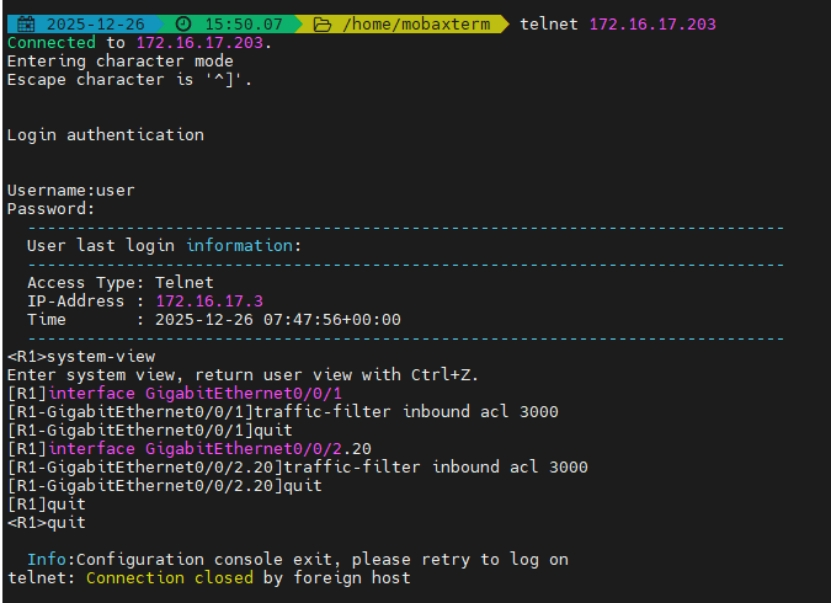
\includegraphics[width=\textwidth]{images/54.jpg}
    \caption{：在R1上应用ACL的配置过程截图。}
\end{figure}

\subsubsection{步骤四：分时段验证ACL策略效果}

\textbf{测试思路}：我们的思路是，选定三个代表性的时间点：（1）\textbf{10:00}（上午时段）、（2）\textbf{15:00}（下午时段）、（3）\textbf{20:00}（其余时段）。在这三个时间点，我们手动修改R1的系统时间，然后立即对5台PC之间进行全面的连通性测试，以验证ACL策略是否按预期生效。

\textbf{(1) 上午时段测试 (10:00)}

\textbf{操作}：将 R1 的系统时间设置为 \texttt{10:00:00}。
\begin{figure}[H]
    \centering
    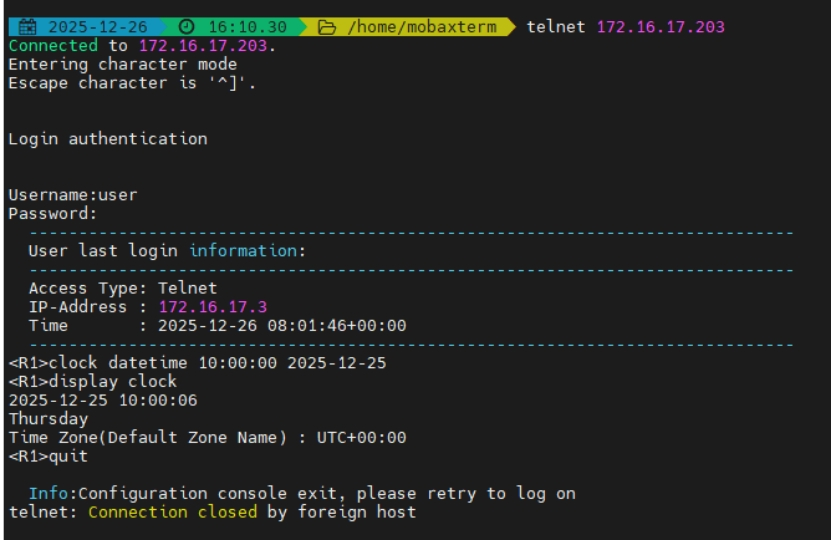
\includegraphics[width=\textwidth]{images/56.jpg}
    \caption{：使用`clock datetime`命令修改R1的系统时间以模拟上午时段。}
\end{figure}

\textbf{测试结果与分析}：

\begin{itemize}
    \item \textbf{H1 测试}:
    \begin{figure}[H]
        \centering
        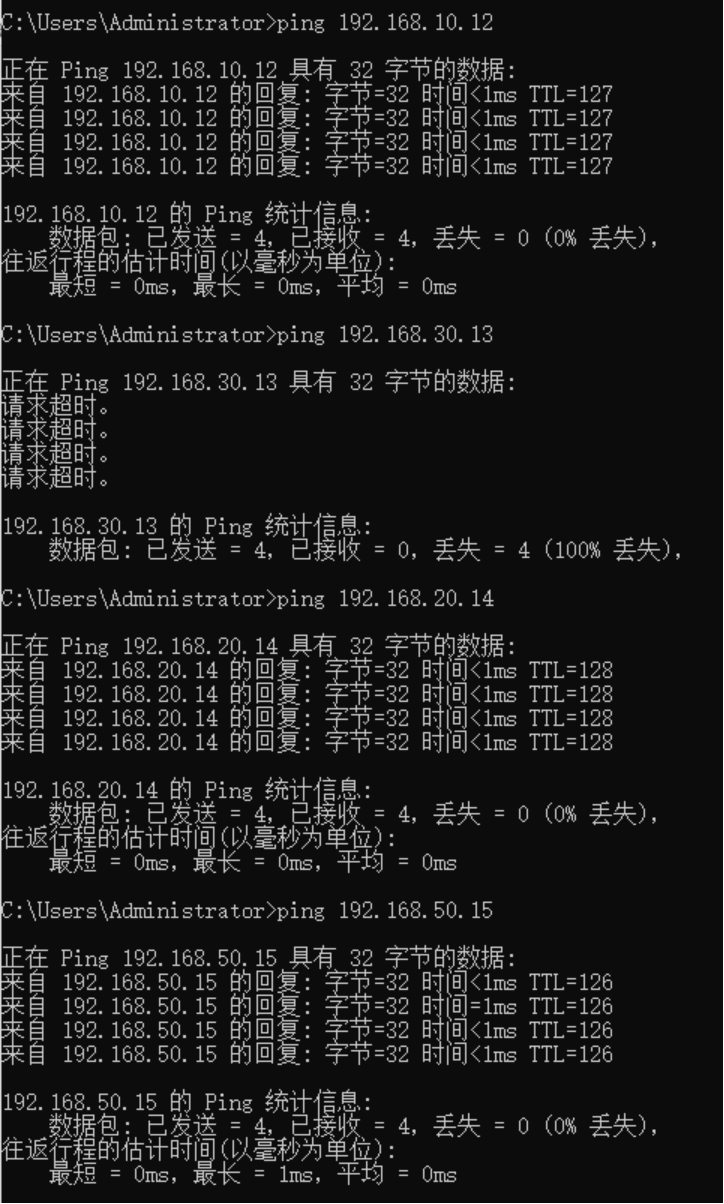
\includegraphics[width=0.75\textwidth]{images/57.jpg}
        \caption{：10:00，H1 ping 其他PC的结果。}
    \end{figure}
    \textbf{结果分析}: H1 ping H2、H4、H5 成功，ping H3 超时，符合预期。H2成功因为 VLAN 10 (H2) 与 VLAN 20 (H1, H4) 之间双向互通，H3失败因为上午时间段 拒绝 H1 与 H3 之间通信，H4 成功因为 H4 与全网任意主机双向互通，H5 成功因为上午时间段允许 H1 与 H5 双向互访。

    \item \textbf{H2 测试}:
    \begin{figure}[H]
        \centering
        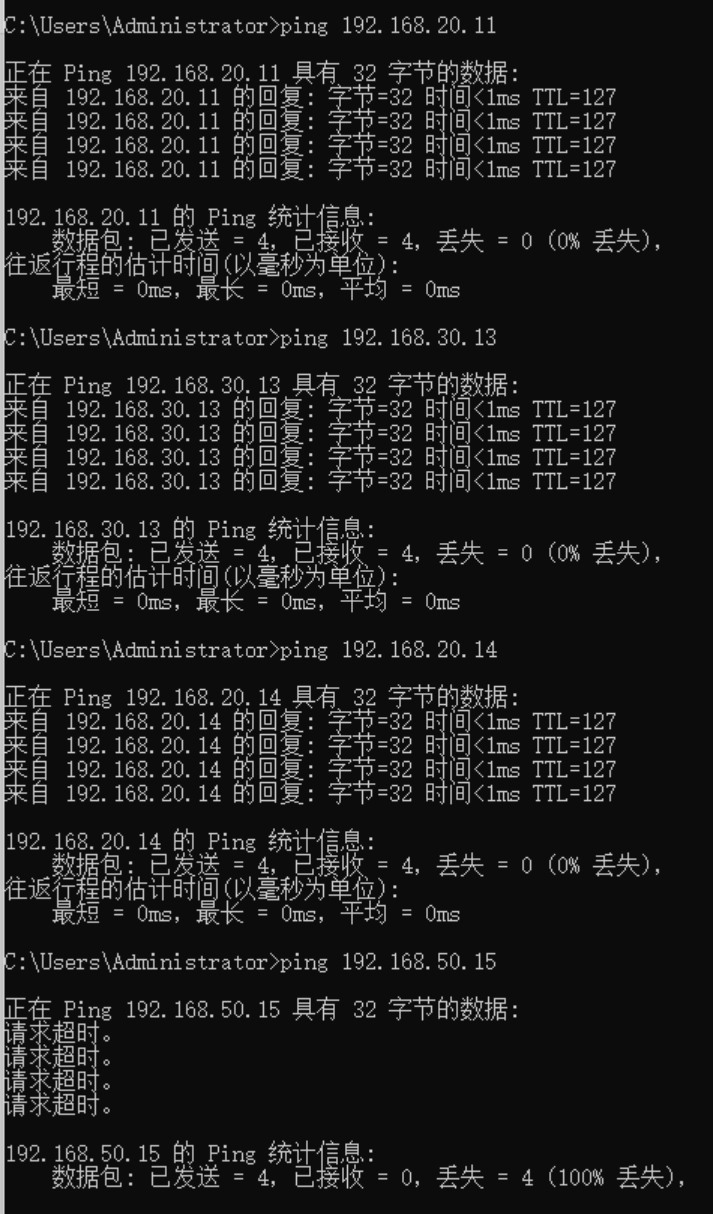
\includegraphics[width=0.70\textwidth]{images/58.jpg}
        \caption{：10:00，H2 ping 其他PC的结果。}
    \end{figure}
    \textbf{结果分析}: H2 ping H1、H3、H4成功，ping H5 超时，符合预期。H1 成功因为VLAN 10 (H2) 与 VLAN 20 (H1, H4) 之间双向互通，H3 成功因为上午时间段允许 H2 与 H3 双向互访，H4 成功因为 H4 与全网任意主机双向互通，H5 超时因为上午时间段拒绝 H2 与 H5 双向访问 。

    \item \textbf{H3 测试}:
    \begin{figure}[H]
        \centering
        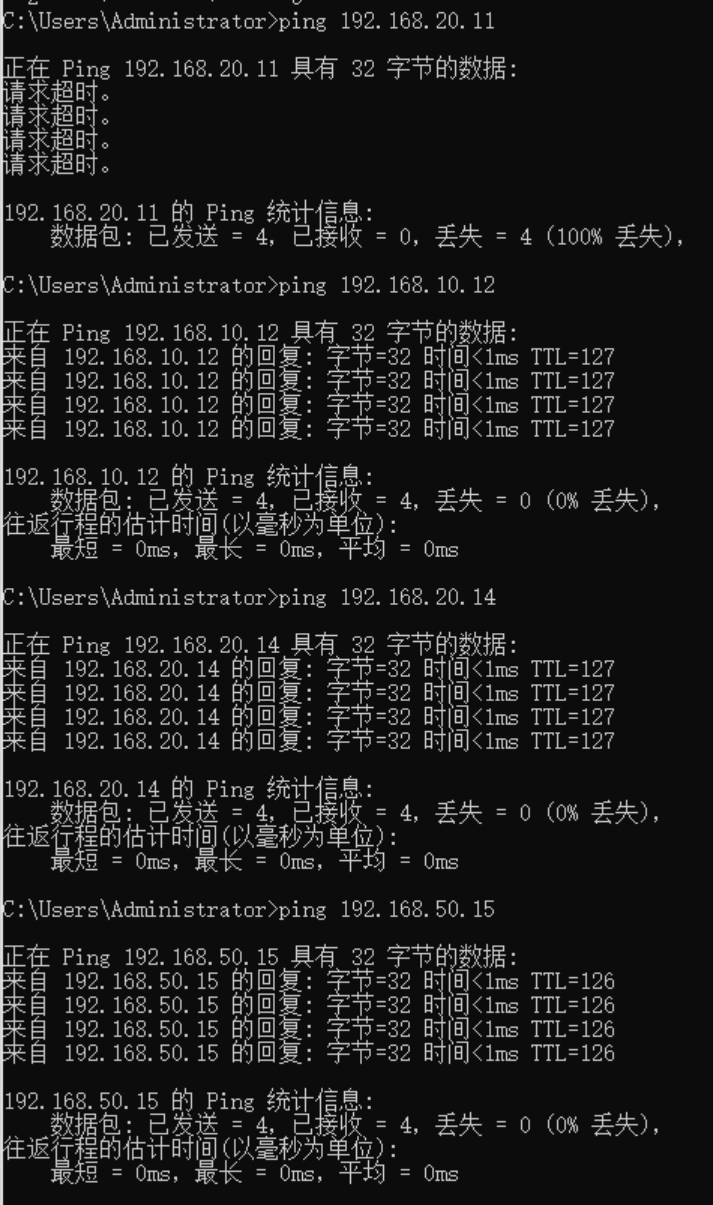
\includegraphics[width=0.70\textwidth]{images/59.jpg}
        \caption{：10:00，H3 ping 其他PC的结果。}
    \end{figure}
    \textbf{结果分析}: H3 ping H2、H4、H5成功，ping H1 超时，符合预期。H1 不通因为上午时间段拒绝 H1 与 H3 双向互访，H2 成功因为上午时间段允许 H2 与 H3 双向互访，H4 成功因为 H4 与全网任意主机双向互通，H5 成功因为 H3 与 H5 双向互通。
    
    \item \textbf{H4 测试}:
    \begin{figure}[H]
        \centering
        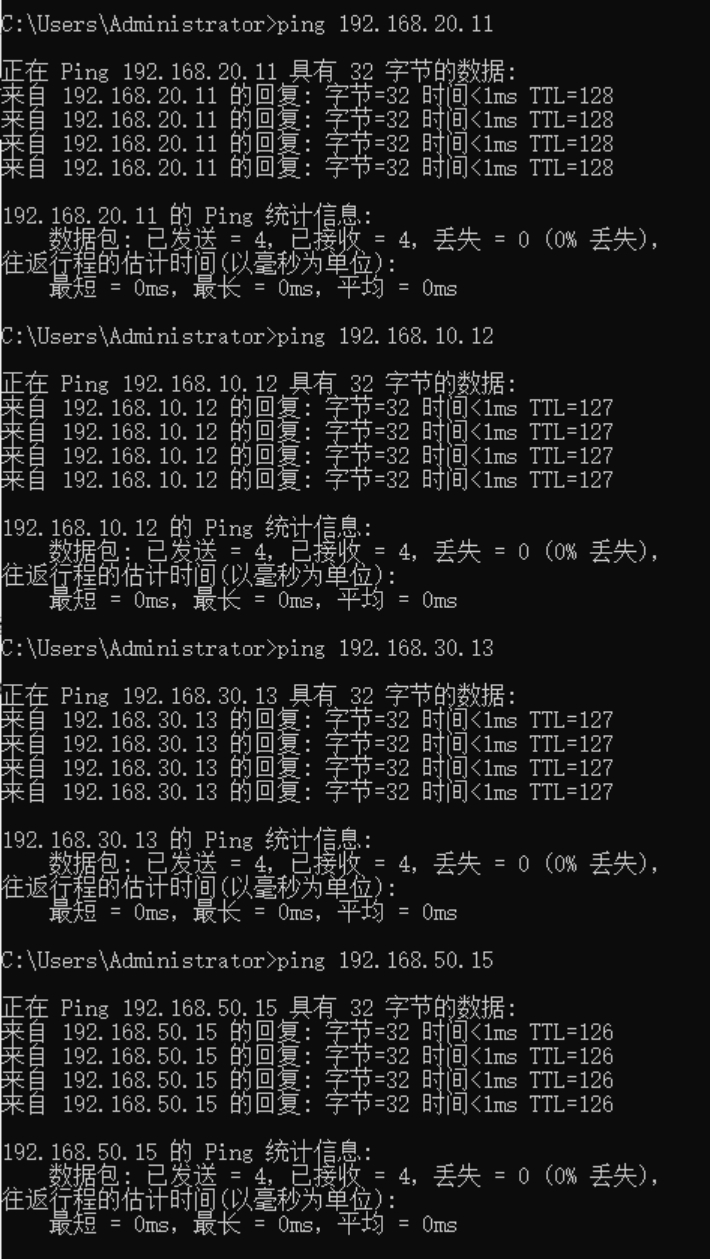
\includegraphics[width=0.75\textwidth]{images/60.jpg}
        \caption{：10:00，H4 ping 其他PC的结果。}
    \end{figure}
    \textbf{结果分析}: H4 ping H1、H2、H3、H5 成功。因为 H4 与全网任意主机双向互通。

    \item \textbf{H5 测试}:
    \begin{figure}[H]
        \centering
        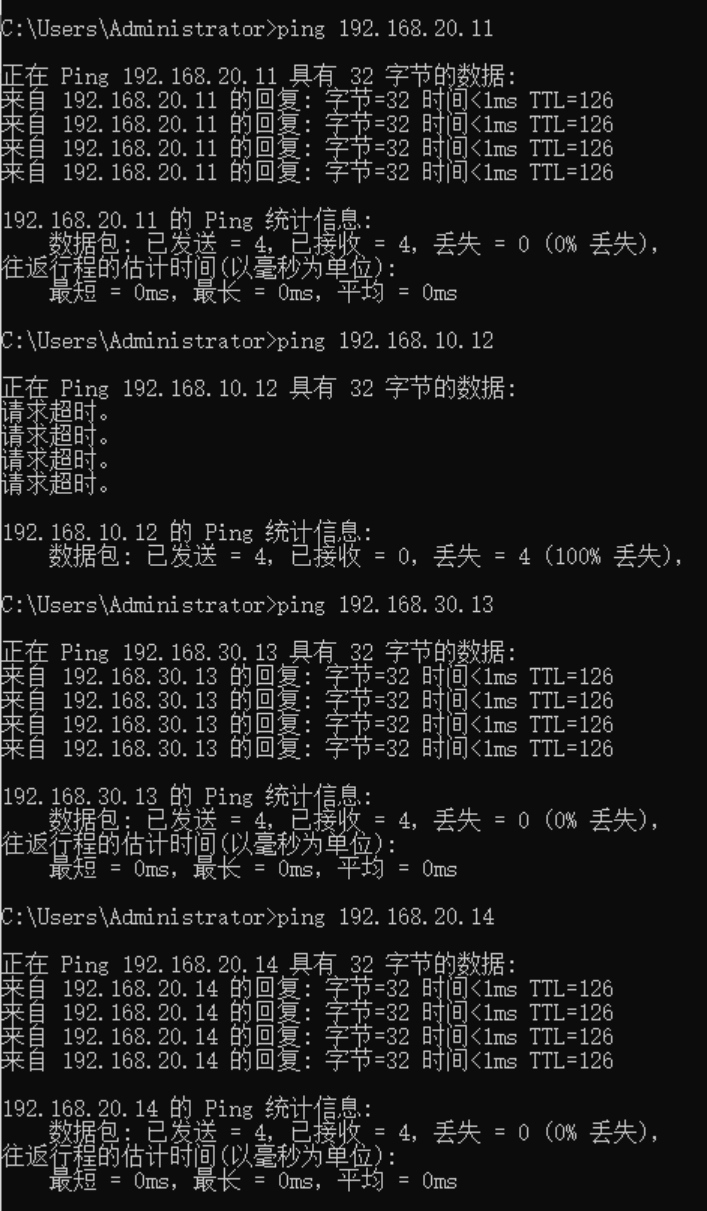
\includegraphics[width=0.70\textwidth]{images/61.jpg}
        \caption{：10:00，H5 ping 其他PC的结果。}
    \end{figure}
    \textbf{结果分析}: H5 ping H1、H3、H4 成功，ping H2 超时，符合预期。H1 成功因为上午时间段允许 H1 与 H5 双向互访，H2 超时因为上午时间段拒绝 H2 与 H5 双向互访，H3 成功因为 H3 与 H5 双向互通，H4 成功因为 H4 与全网任意主机双向互通。
\end{itemize}

\textbf{(2) 下午时段测试 (15:00)}

\textbf{操作}：将R1的系统时间设置为\texttt{15:00:00}。
\begin{figure}[H]
    \centering
    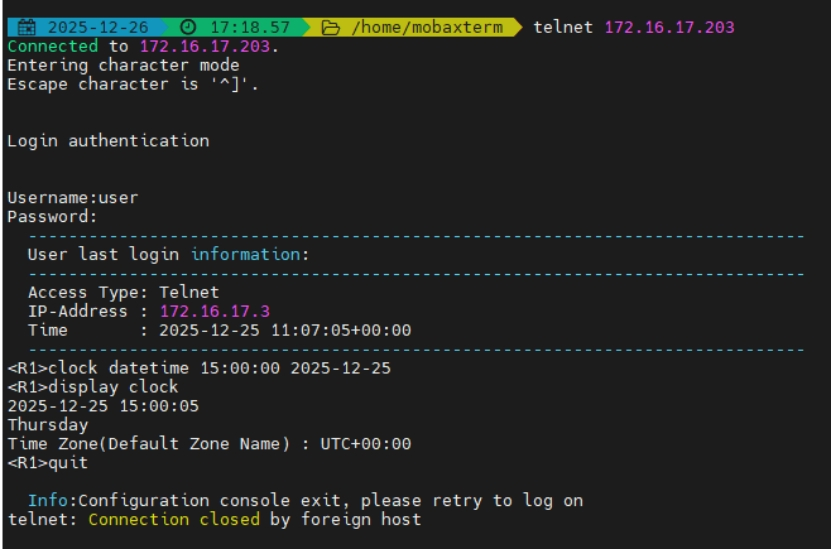
\includegraphics[width=\textwidth]{images/62.jpg}
    \caption{：修改R1系统时间以模拟下午时段。}
\end{figure}

\textbf{测试结果与分析}：

\begin{itemize}
    \item \textbf{H1 测试}:
    \begin{figure}[H]
        \centering
        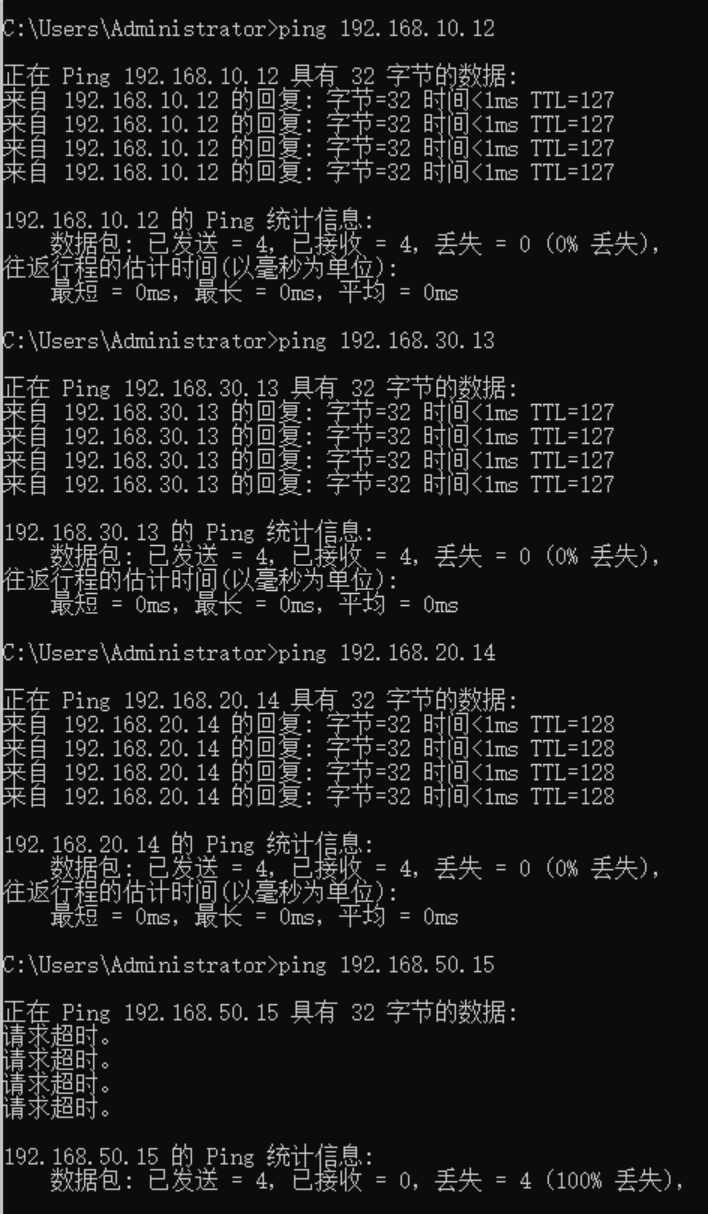
\includegraphics[width=0.72\textwidth]{images/63.jpg}
        \caption{：15:00，H1 ping 其他PC的结果。}
    \end{figure}
    \textbf{结果分析}: H1 ping H2、H3、H4成功，ping H5 超时，符合预期。H2 成功因为 VLAN 10 (H2) 与 VLAN 20 (H1, H4) 之间双向互访，H3 成功下午时间段允许 H1 与 H3 双向互访，H4 成功 H4 与全网任意主机双向互通，H5 超时因为下午时间段 拒绝 H1 与 H5双向互访。

    \item \textbf{H2 测试}:
    \begin{figure}[H]
        \centering
        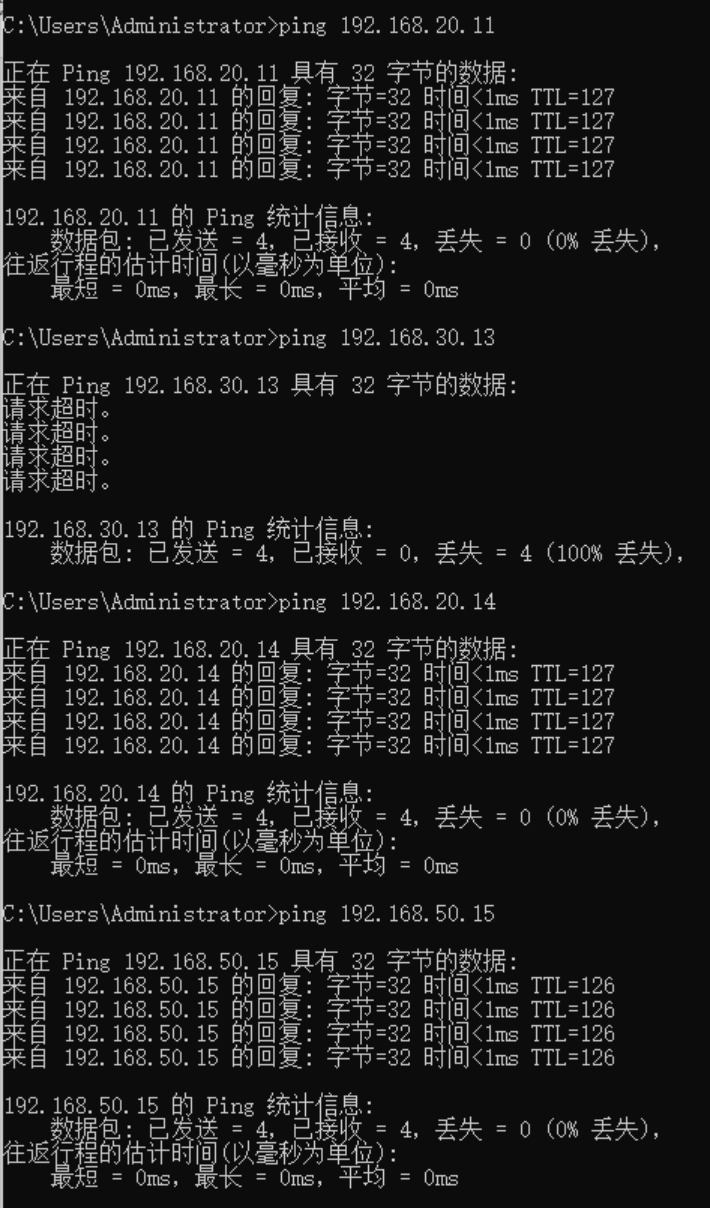
\includegraphics[width=0.70\textwidth]{images/64.jpg}
        \caption{：15:00，H2 ping 其他PC的结果。}
    \end{figure}
    \textbf{结果分析}: H2 ping H1、H4、H5，ping H3 超时，符合预期。H1成功因为VLAN 10 (H2) 与 VLAN 20 (H1, H4) 之间双向互访，H3 超时因为下午时间段拒绝 H2 与 H3 双向互访，H4 成功因为 H4 与全网任意主机双向互通，H5 成功因为下午时间段允许 H2 与 H5 双向互访。
    
    \item \textbf{H3, H4, H5 测试}:
    \begin{figure}[H]
        \centering
        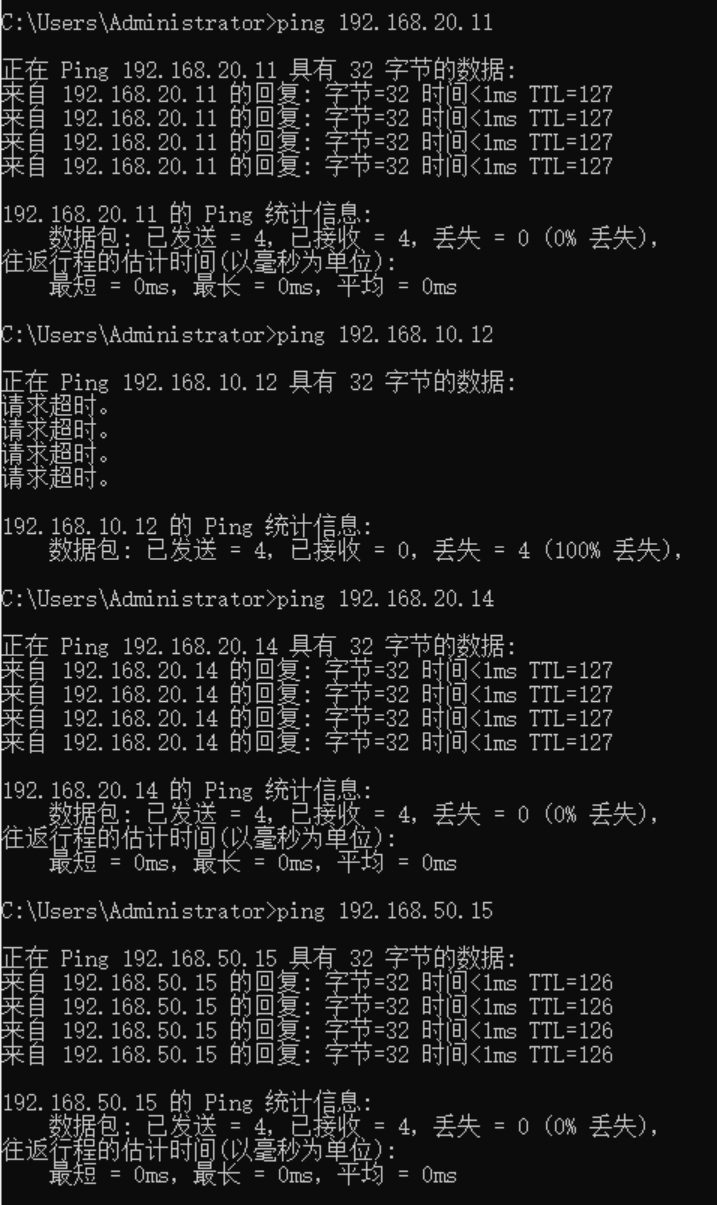
\includegraphics[width=0.80\textwidth]{images/65.jpg}
        \caption{：15:00，H3 ping 其他PC的结果。}
    \end{figure}
    \begin{figure}[H]
        \centering
        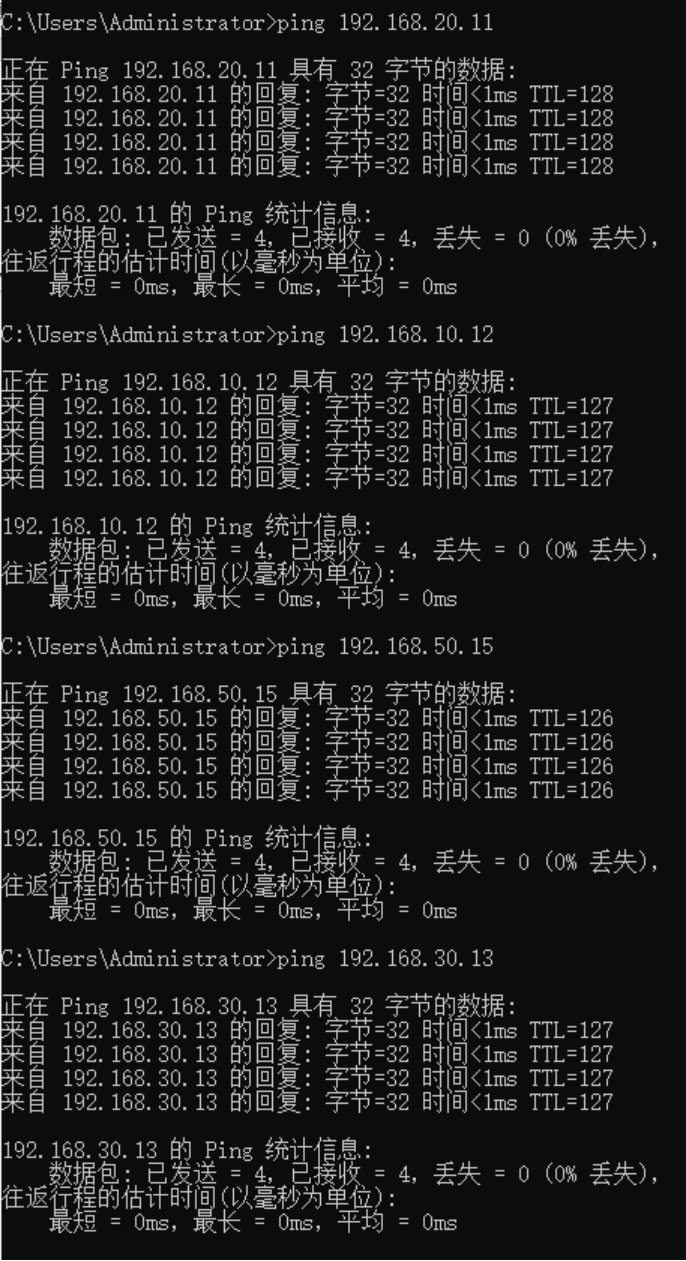
\includegraphics[width=0.80\textwidth]{images/66.jpg}
        \caption{：15:00，H4 ping 其他PC的结果。}
    \end{figure}
    \begin{figure}[H]
        \centering
        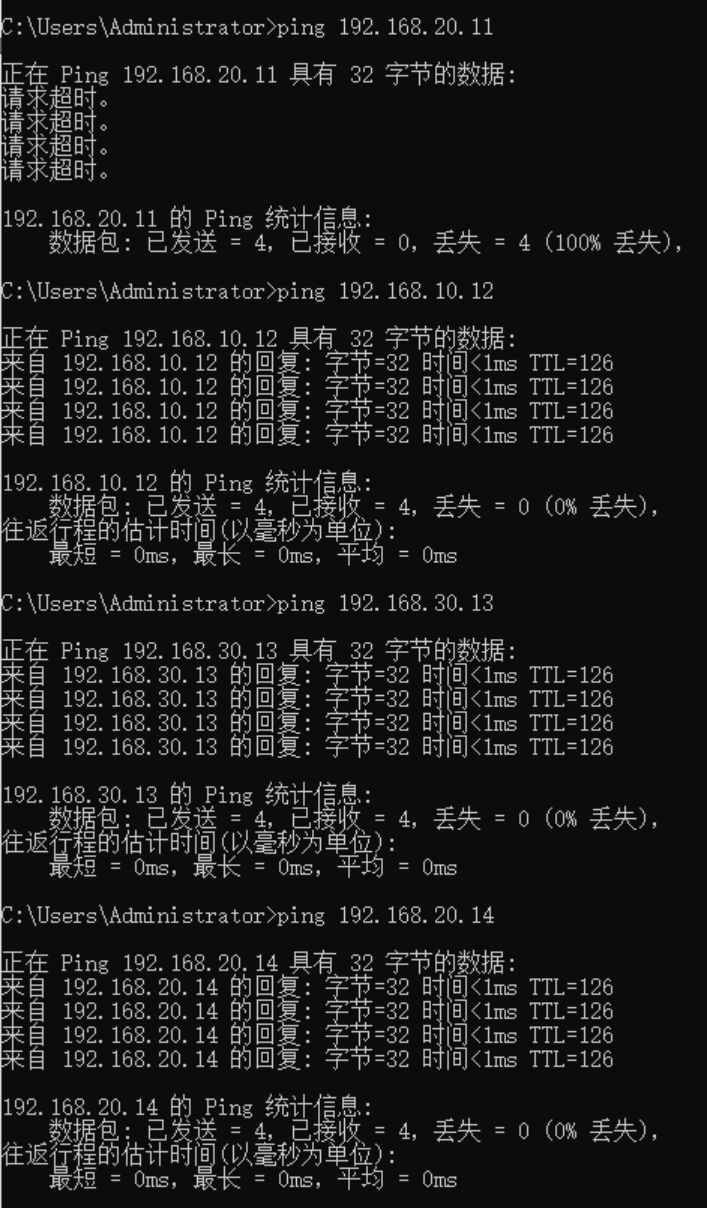
\includegraphics[width=0.80\textwidth]{images/67.jpg}
        \caption{：15:00，H5 ping 其他PC的结果。}
    \end{figure}
    \textbf{结果分析}: H3, H4, H5的测试结果（如图65, 66, 67）均与H1/H2的测试结果对称，全面验证了下午时段策略的正确性。
\end{itemize}

\textbf{(3) 其余时段测试 (20:00)}

\textbf{操作}：将R1的系统时间设置为\texttt{20:00:00}。
\begin{figure}[H]
    \centering
    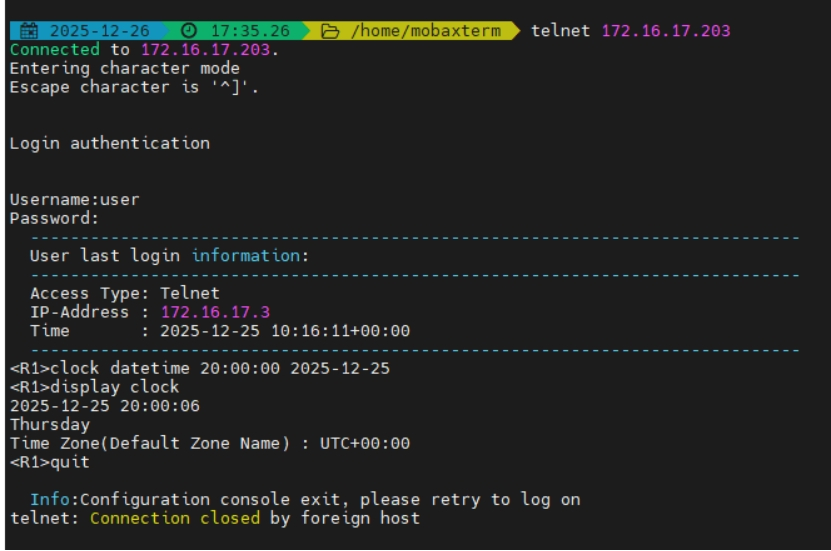
\includegraphics[width=\textwidth]{images/68.jpg}
    \caption{：修改R1系统时间以模拟“其余时段”。}
\end{figure}

\textbf{测试结果与分析}：

\begin{itemize}
    \item \textbf{H1 测试}:
    \begin{figure}[H]
        \centering
        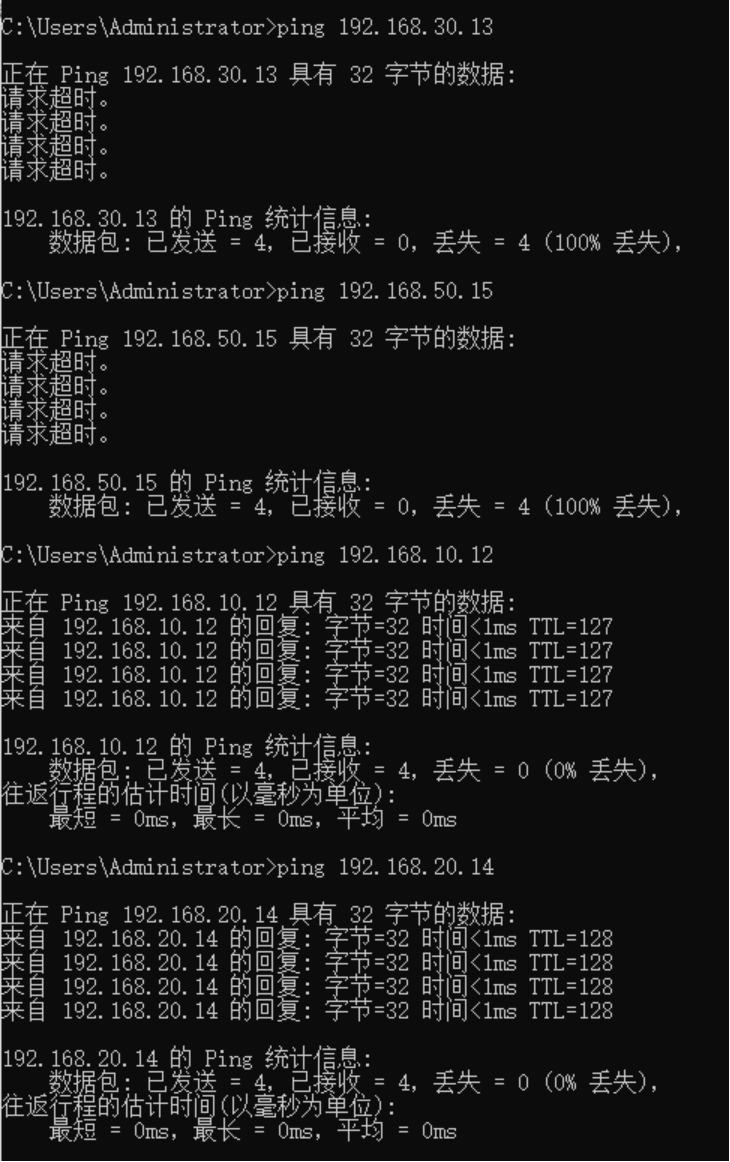
\includegraphics[width=0.75\textwidth]{images/69.jpg}
        \caption{：20:00，H1 ping 其他PC的结果。}
    \end{figure}
    \textbf{结果分析}: H1 ping H2、H4 成功，ping H3、H5 超时，符合预期。H2 成功因为VLAN 10 (H2) 与 VLAN 20 (H1, H4) 之间双向互访，H3 超时因为其余时间禁止 H1 与 H3 双向互访，H4 成功因为 H4 与全网任意主机双向互通，H5 超时因为其余时间禁止 H1 与 H5 双向互访。

    \item \textbf{H2 测试}:
    \begin{figure}[H]
        \centering
        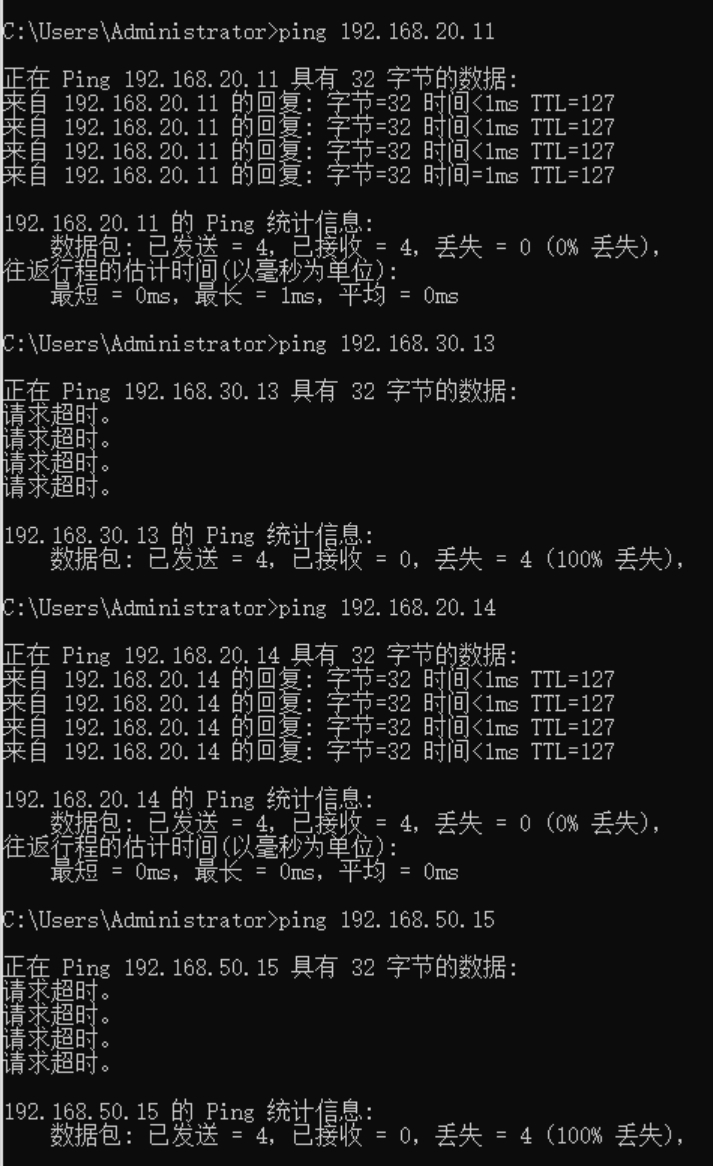
\includegraphics[width=0.72\textwidth]{images/70.jpg}
        \caption{：20:00，H2 ping 其他PC的结果。}
    \end{figure}
    \textbf{结果分析}: H2 ping H1、H4 成功，ping H3、H5超时，符合预期。H1 成功因为VLAN 10 (H2) 与 VLAN 20 (H1, H4) 之间双向互访，H3 超时因为其余时间禁止 H2 与 H3 双向互访，H4 成功因为 H4 与全网任意主机双向互通，H5 超时因为其余时间禁止 H2 与 H5 双向互访。

    \item \textbf{H3, H4, H5 测试}:
    \begin{figure}[H]
        \centering
        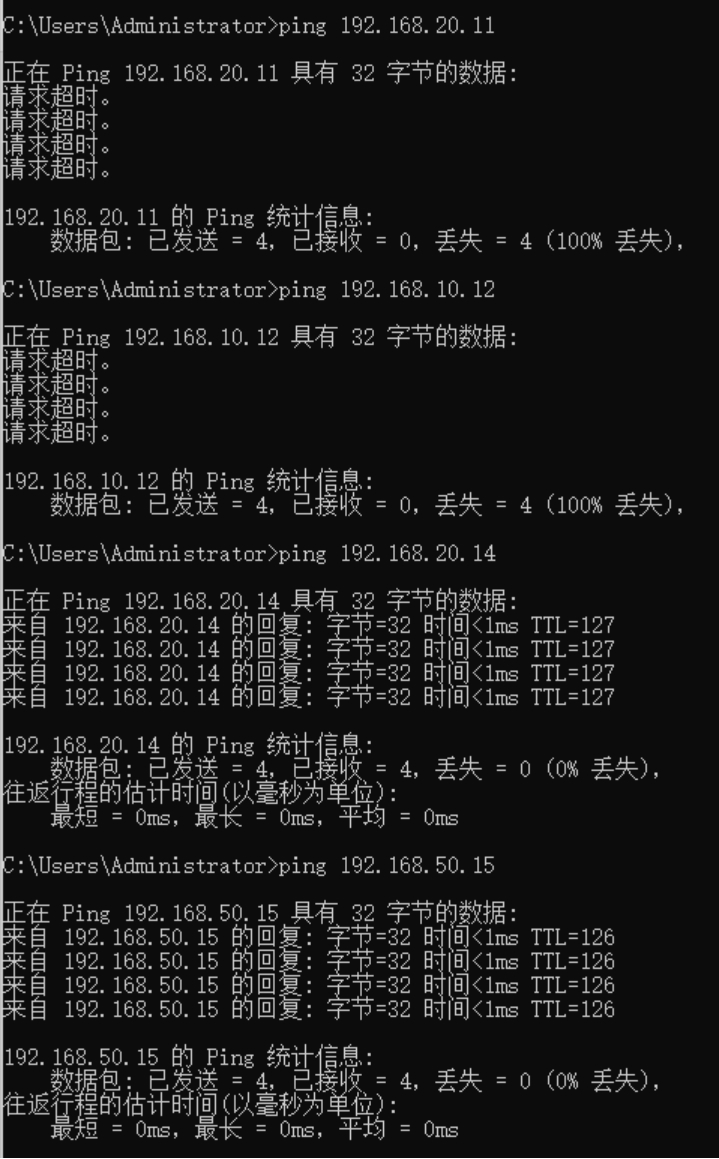
\includegraphics[width=0.80\textwidth]{images/71.jpg}
        \caption{：20:00，H3 ping 其他PC的结果。}
    \end{figure}
    \begin{figure}[H]
        \centering
        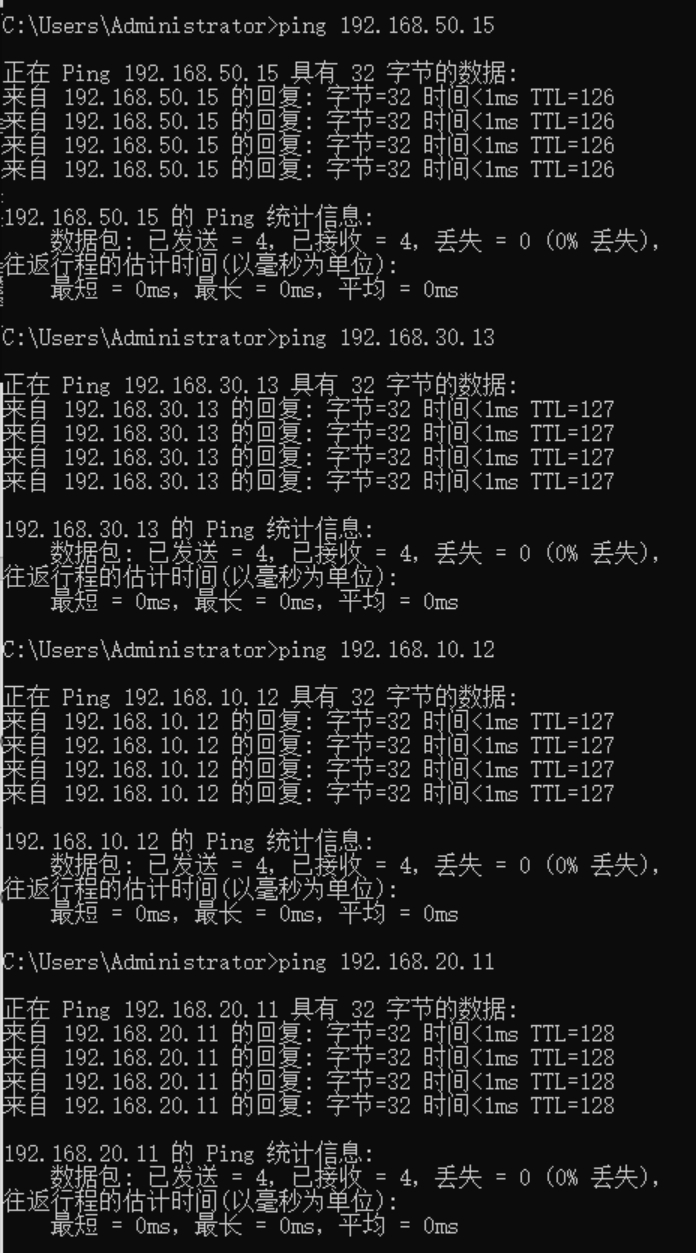
\includegraphics[width=0.80\textwidth]{images/72.jpg}
        \caption{：20:00，H4 ping 其他PC的结果。}
    \end{figure}
    \begin{figure}[H]
        \centering
        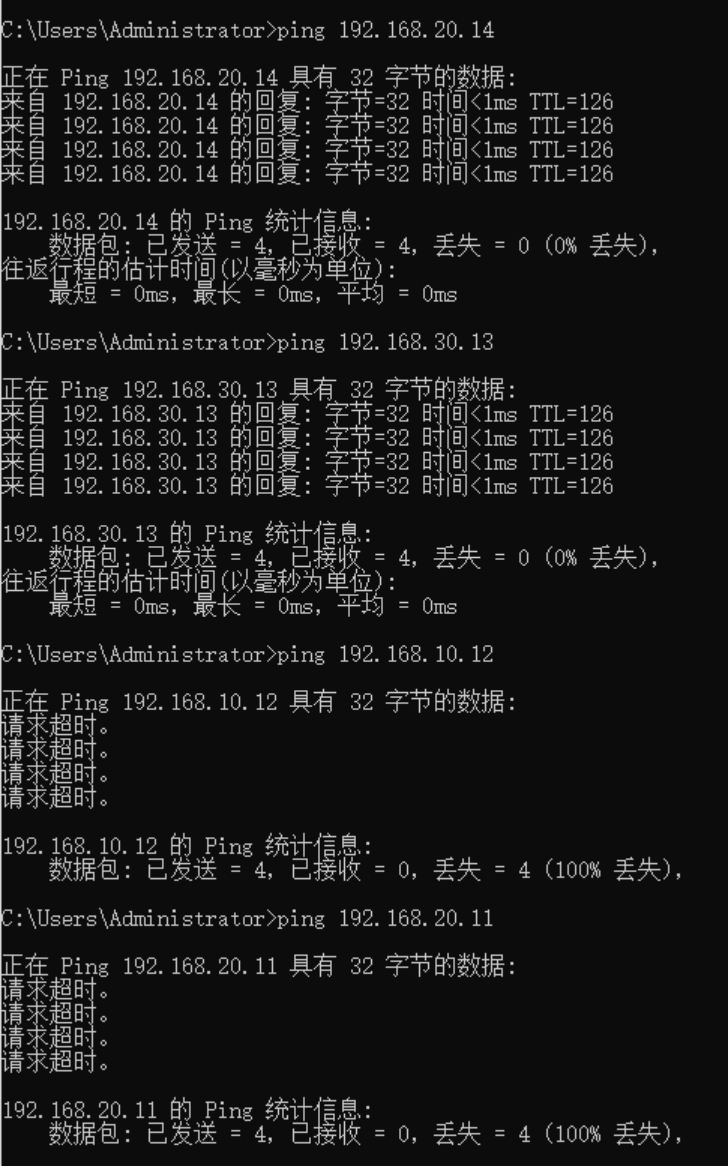
\includegraphics[width=0.80\textwidth]{images/73.jpg}
        \caption{：20:00，H5 ping 其他PC的结果。}
    \end{figure}
    \textbf{结果分析}: H3, H4, H5的测试结果（如图71, 72, 73）再次呈现对称性，所有在“其余时段”受限的通信均被有效阻止，而不受限的“特权”通信（如H3-H5, H4-任意）则保持畅通。
\end{itemize}

\subsection{总结}

本任务在路由器 R1 上部署了结合 \texttt{time-range} 的 ACL 规则集。通过在三个不同时间点进行的点到点测试，确认了访问控制策略已按要求生效，精确控制了不同主机在指定时间段内的通信权限。

\newpage
\section{任务五：基于TCP的图像与文字传输及路径分析}

\subsection{实验要求}

本任务要求基于TCP套接字编程技术，实现H1（发送端）向H5（接收端）传输指定的图像和文字数据。核心任务包括：

\begin{enumerate}
    \item \textbf{实现数据传输}：由主机 H1 作为发送端（客户端），向主机 H5（接收端/服务器）发送指定的数据，内容包括一张BMP格式的图像和一段英文文字。
    \item \textbf{路径特征分析}：通过在传输路径上的关键网络设备（S1, S2, R1, R2）上配置端口镜像并进行抓包，捕获数据包在经过交换机和路由器时的状态变化，重点分析MAC地址、IP地址及TTL等字段的特点。
    \item \textbf{验证传输可靠性}：在接收端 H5 比较接收到的图像和文字数据，与发送端 H1 的原始版本进行比对，以验证TCP协议的可靠传输机制。
\end{enumerate}

\subsection{实验设计与流程规划}

为达成上述目标，我们制定了实验方案，涵盖了网络准备、多点抓包部署、程序设计与实现、数据传输验证以及深度路径分析等多个环节。

\begin{enumerate}
    \item \textbf{协议选择}：实验要求在UDP或TCP中选择。考虑到需要传输文件（图像）并确保其完整性，我们选择\textbf{TCP协议}。TCP是面向连接的、可靠的传输层协议，它通过序列号、确认应答、超时重传等机制，能够保证数据不丢失、不重复、无差错且按序到达，符合本任务要求。
    \item \textbf{应用层协议设计}：为在同一个TCP连接上清晰地区分图像和文字两种不同类型的数据，我们设计了一个简单的应用层协议。在发送任何实际数据之前，客户端先发送一个8字节的固定长度头部，其中前4字节表示数据类型（1代表图片，2代表文字），后4字节表示紧随其后的数据负载的长度。服务器端据此头部信息来准确地接收和处理数据，有效避免了TCP粘包问题。
    \item \textbf{多点抓包方案}：为了完整地追踪数据包从H1到H5的传输路径，我们在路径上的每一台中间设备上都配置了端口镜像作为观测点。通过在S1, S2, R1, R2上配置端口镜像，我们将数据流的“入口”和“出口”流量都复制到指定的观察主机（H2, H3, H4, H6）上，并使用Wireshark进行捕获。这个方案使我们能够分析数据包在每一跳（hop）上的二层（MAC地址）和三层（TTL）头部变化。
    \item \textbf{执行与验证流程}：
    \begin{itemize}
        \item (1) 暂时移除任务四中配置的 ACL 策略，确保 H1 到 H5 之间路由畅通。
        \item (2) 在所有中间设备上配置端口镜像，并在各观察主机上启动 Wireshark。
        \item (3) 在 H5 上运行服务器端 Python 脚本，使其进入监听状态。
        \item (4) 在 H1 上运行客户端 Python 脚本，触发图像和文字的发送。
        \item (5) 在 H5 上验证接收文件的完整性（通过 MD5 哈希值比对），并停止抓包，对捕获的数据进行逐跳分析。
    \end{itemize}
\end{enumerate}

\subsection{实验步骤与结果分析}

\subsubsection{步骤一：网络环境准备与基线测试}

\textbf{操作目的}：在进行数据传输之前，必须确保H1与H5之间的网络路径是完全可达的。任务四部署的ACL策略会干扰本次实验的正常通信，因此需要暂时将其移除，构建一个干净的测试环境。

\textbf{操作描述}：我们通过Telnet登录到路由器R1，进入其连接VLAN 10和VLAN 20的两个网关接口（物理接口GE0/0/1和子接口GE0/0/2.20），使用\texttt{undo traffic-filter inbound}命令，将之前应用的ACL 3000策略从接口的入方向上解绑。

\begin{lstlisting}[language=bash, caption={: 通过`undo traffic-filter`命令，我们移除了应用于VLAN 10和VLAN 20网关接口入方向的ACL 3000，从而恢复了路由器的默认转发行为。}]
system-view
interface GigabitEthernet0/0/1
 undo traffic-filter inbound
quit
interface GigabitEthernet0/0/2.20
 undo traffic-filter inbound
quit
save
\end{lstlisting}

\begin{figure}[H]
    \centering
    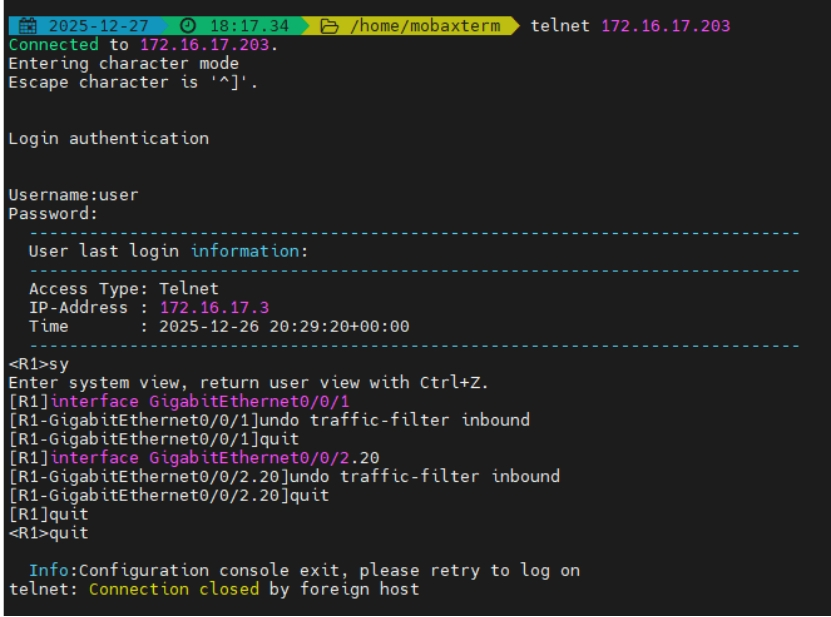
\includegraphics[width=\textwidth]{images/74.jpg}
    \caption{在R1上执行命令解绑ACL的过程截图}
\end{figure}

\textbf{基线连通性测试}：完成ACL解绑后，我们立即在H1和H5上进行双向\texttt{ping}测试，以验证网络的端到端连通性。

\begin{figure}[H]
    \centering
    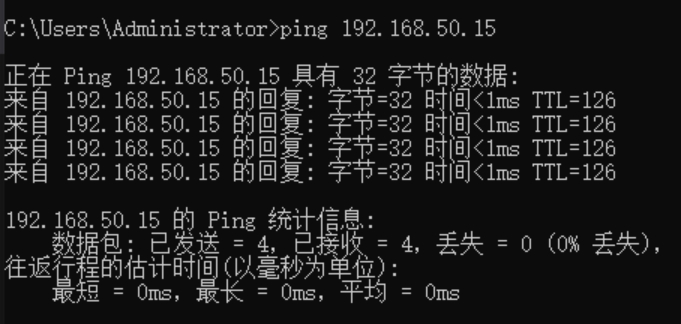
\includegraphics[width=0.7\textwidth]{images/75.jpg}
    \caption{H1 ping H5 的测试结果}
\end{figure}

\begin{figure}[H]
    \centering
    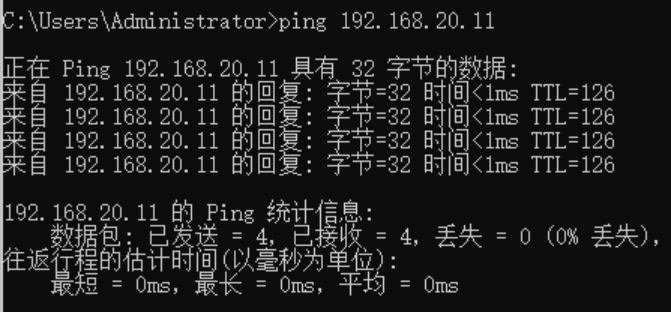
\includegraphics[width=0.7\textwidth]{images/76.jpg}
    \caption{H5 ping H1 的测试结果}
\end{figure}

\textbf{结果分析}：如上图所示，H1与H5之间可以正常双向\texttt{ping}通，且无任何丢包。值得注意的是，\texttt{ping}命令的回显信息中 \texttt{TTL=126}。通常Windows主机的IP包初始TTL值为128，现在变为126，说明数据包在传输路径中经过了 \texttt{128 - 126 = 2} 个路由器。这与我们的拓扑结构（H1 $\rightarrow$ S1 $\rightarrow$ S2 $\rightarrow$ \textbf{R1} $\rightarrow$ \textbf{R2} $\rightarrow$ H5）完全吻合。这个简单的测试不仅确认了网络全通，也为我们后续的TTL变化分析提供了一个准确的基准。

\subsubsection{步骤二：部署多点端口镜像以备抓包}

\textbf{操作目的}：为了能够捕获数据包在网络中传输时的真实状态，我们需要在路径上的每一台交换机和路由器上部署端口镜像。该技术可以将指定端口的流量（入方向、出方向或双向）复制一份到另一个“观察端口”，连接在该观察端口上的主机即可对这些流量进行分析。

\textbf{分析与思考}：
本任务需要观察数据包在网络传输过程中的变形。一个IP包从源H1发出，到目的H5接收，会依次经过S1、S2、R1、R2。为了捕获它在每一跳设备上的状态，我们需要在这些设备上设置端口镜像。

我们的抓包点设计如下，捕获每一段关键链路上的流量：
\begin{itemize}
    \item \textbf{在S1抓包}：使用H2作为抓包机，镜像H1的\textbf{入向}流量和去往S2的\textbf{出向}流量。这能让我们看到数据包最原始的样子，以及它第一次被交换机转发时的状态。
    \item \textbf{在S2抓包}：使用H4作为抓包机，镜像从S1来的\textbf{入向}流量和去往R1的\textbf{出向}流量。这能看到数据包跨越交换机后的状态。
    \item \textbf{在R1抓包}：使用H3作为抓包机，镜像从S2来的\textbf{入向}流量和去往R2的\textbf{出向}流量。这是观察第一次三层转发（MAC地址改变、TTL减1）的关键节点。
    \item \textbf{在R2抓包}：使用一台额外的主机H6作为抓包机，镜像从R1来的\textbf{入向}流量和去往H5的\textbf{出向}流量。这是观察第二次三层转发的关键节点。
\end{itemize}

\textbf{操作描述}：我们按照上述思路，在四台网络设备上分别配置端口镜像。

\textbf{S1 镜像配置 (telnet 172.16.17.201):}

\begin{itemize}
    \item \textbf{抓包机}：H2（临时连接至S1的GE0/0/2口）
    \item \textbf{监控目标}：镜像从H1进入S1的流量（\texttt{GE0/0/1 inbound}）和从S1转发至S2的流量（\texttt{GE0/0/22 outbound}）。
\end{itemize}

\begin{lstlisting}[language=bash, caption={: 在S1上，将H1入向流量和去往S2的出向流量都复制到观察端口GE0/0/2。}]
system-view
! 1. 指定GE0/0/2为观察端口
observe-port 1 interface GigabitEthernet 0/0/2
! 2. 镜像H1的入站流量
interface GigabitEthernet0/0/1
 port-mirroring to observe-port 1 inbound
quit
! 3. 镜像去往S2的主链路的出站流量
interface GigabitEthernet0/0/22
 port-mirroring to observe-port 1 outbound
quit
save
\end{lstlisting}

\begin{figure}[H]
    \centering
    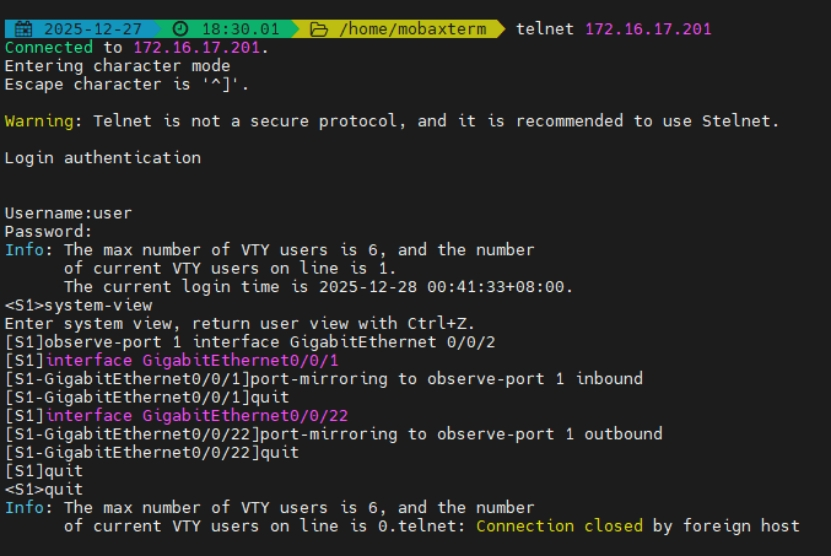
\includegraphics[width=\textwidth]{images/77.jpg}
    \caption{S1镜像配置过程截图}
\end{figure}

\textbf{S2 镜像配置}：

\begin{itemize}
    \item \textbf{抓包机}：H4（连接至S2的GE0/0/2口）
    \item \textbf{监控目标}：镜像从S1到达S2的流量（\texttt{GE0/0/22 inbound}）和从S2转发至R1的流量（\texttt{GE1/0/24 outbound}）。
\end{itemize}

\begin{lstlisting}[language=bash, caption={: 在S2上，将从S1来的入向流量和去往R1的出向流量复制到H4所在的观察端口。}]
system-view
! 1. 指定GE0/0/2为观察端口
observe-port 1 interface GigabitEthernet 0/0/2
! 2. 镜像从S1主链路来的入站流量
interface GigabitEthernet1/0/22
 port-mirroring to observe-port 1 inbound
quit
! 3. 镜像去往R1的出站流量
interface GigabitEthernet1/0/24
 port-mirroring to observe-port 1 outbound
quit
save
\end{lstlisting}

\begin{figure}[H]
    \centering
    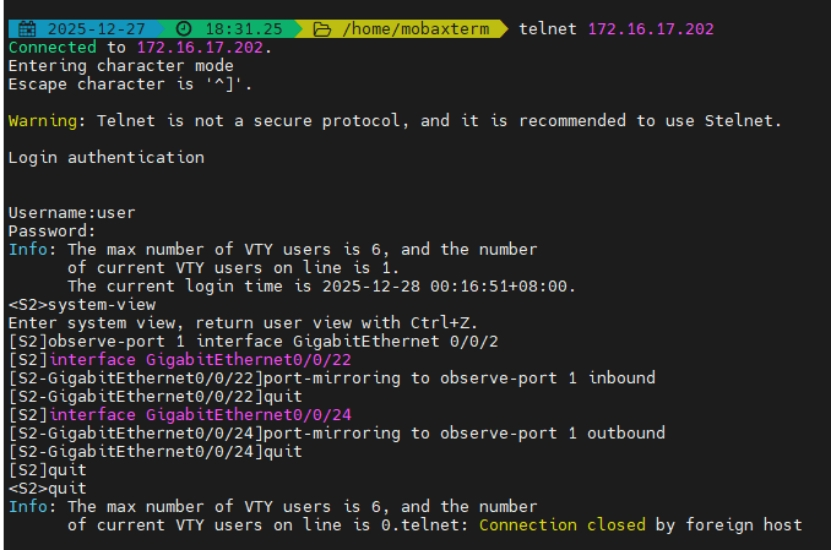
\includegraphics[width=\textwidth]{images/78.jpg}
    \caption{S2镜像配置过程截图}
\end{figure}

\textbf{R1 镜像配置}：

\begin{itemize}
    \item \textbf{抓包机}：H3（连接至R1的GE0/0/3口）
    \item \textbf{监控目标}：镜像从S2到达R1的流量（\texttt{GE0/0/2 inbound}）和从R1转发至R2的流量（\texttt{GE0/0/0 outbound}）。
\end{itemize}

\begin{lstlisting}[language=bash, caption={: 在R1上，将从S2来的入向流量和去往R2的出向流量复制到H3所在的观察端口。}]
system-view
! 1. 指定GE0/0/3为观察端口
observe-port interface GigabitEthernet 0/0/3
! 2. 镜像从S2来的入站流量
interface GigabitEthernet 0/0/2
 mirror to observe-port inbound
quit
! 3. 镜像去往R2的出站流量
interface GigabitEthernet 0/0/0
 mirror to observe-port outbound
quit
save
\end{lstlisting}

\begin{figure}[H]
    \centering
    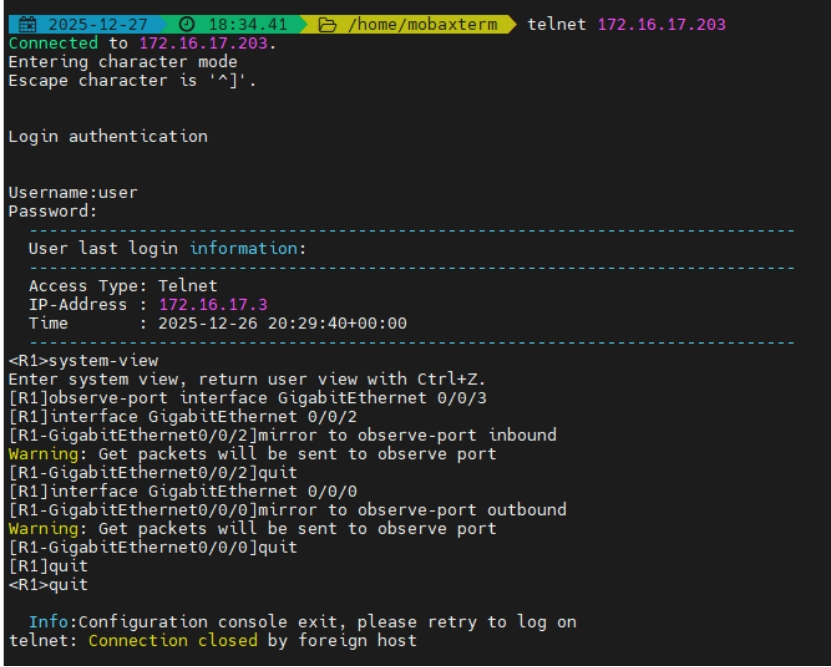
\includegraphics[width=\textwidth]{images/79.jpg}
    \caption{R1镜像配置过程截图。注意路由器镜像命令语法与交换机略有不同。}
\end{figure}

\textbf{R2 镜像配置}：

\begin{itemize}
    \item \textbf{抓包机}：H6（一台额外的PC，连接至R2的GE0/0/6口）
    \item \textbf{监控目标}：镜像从R1到达R2的流量（\texttt{GE0/0/4 inbound}）和从R2转发至H5的流量（\texttt{GE0/0/5 outbound}）。
\end{itemize}

\begin{lstlisting}[language=bash, caption={: 在R2上，将从R1来的入向流量和去往H5的出向流量复制到H6所在的观察端口。}]
system-view
! 1. 指定GE0/0/6为观察端口
observe-port interface GigabitEthernet 0/0/6
! 2. 镜像从R1来的入站流量
interface GigabitEthernet 0/0/4
 mirror to observe-port inbound
quit
! 3. 镜像去往H5的出站流量
interface GigabitEthernet 0/0/5
 mirror to observe-port outbound
quit
save
\end{lstlisting}

\begin{figure}[H]
    \centering
    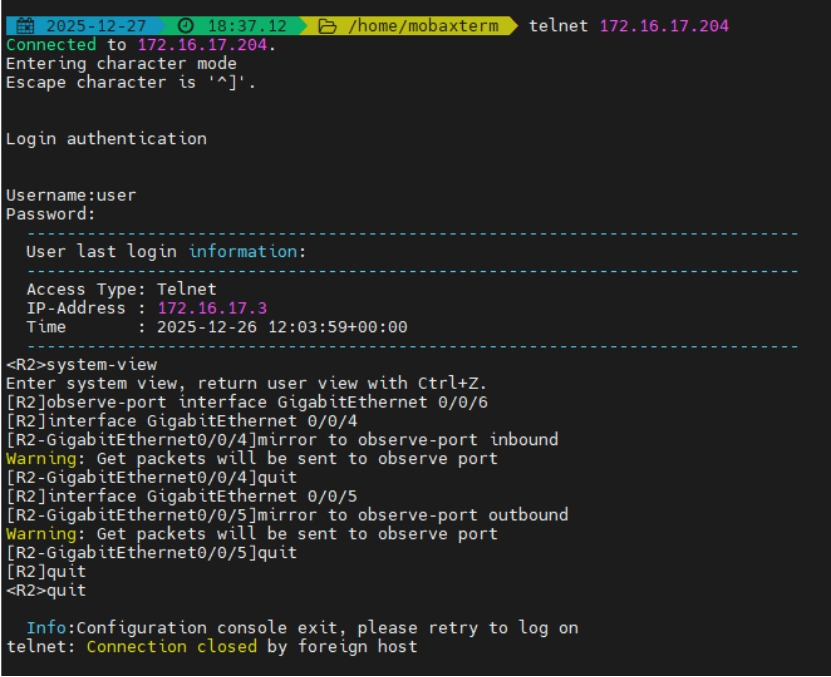
\includegraphics[width=\textwidth]{images/80.jpg}
    \caption{R2镜像配置过程截图}
\end{figure}

\textbf{分析}：通过以上配置，我们构建了一个覆盖全程的流量监控网络。
现在，H1、H2、H3、H4、H5、H6六台主机各司其职，准备从不同视角记录即将发生的数据传输过程。

\subsubsection{步骤三：Socket程序设计与实现}

\textbf{操作目的}：编写客户端和服务器端程序，以实现基于TCP的、包含自定义应用层协议的数据传输功能。

\textbf{分析与思考}：
为了可靠地传输图像和文字两种不同类型的数据，我们要设计一个简单的应用层协议。
直接发送原始数据流可能导致粘包问题，接收方无法区分数据流中哪部分是图片，哪部分是文字。

我们的解决方案是\textbf{头部+数据}的封装格式：
\begin{itemize}
    \item \textbf{头部}：定义一个8字节的定长头部。前4字节表示数据类型（例如，1代表图片，2代表文字），后4字节表示紧随其后的数据负载的长度。
    \item \textbf{数据}：实际的图片或文字数据。
\end{itemize}
这样，服务器端在接收时，总是先读取8字节的头部，解析出数据类型和长度，然后再根据长度准确地读取相应大小的数据块，从而有效地解决了粘包问题。

\textbf{服务器端代码 (TCPServer.py, 运行于H5)}：

\begin{lstlisting}[language=python, caption={H5服务器端Python代码}]
import socket
import struct

HOST = ''  # 监听所有可用接口
PORT = 12345 # 使用一个非特权端口

with socket.socket(socket.AF_INET, socket.SOCK_STREAM) as s:
    s.bind((HOST, PORT))
    s.listen()
    print(f"[SERVER] Listening on port {PORT}...")
    conn, addr = s.accept()
    with conn:
        print(f"[SERVER] Connected by {addr}")
        while True:
            # 1. 接收8字节的固定头部
            header = conn.recv(8)
            if not header:
                break
            
            # 2. 解包头部，获取数据类型和数据长度
            data_type, data_len = struct.unpack('!II', header)

            # 3. 根据长度接收完整数据
            data = b''
            while len(data) < data_len:
                packet = conn.recv(data_len - len(data))
                if not packet:
                    break
                data += packet

            # 4. 根据类型处理数据
            if data_type == 1: # 类型1代表图片
                with open("received_logo.bmp", "wb") as f:
                    f.write(data)
                print(f"[SERVER] Received and saved image file ('received_logo.bmp').")
            elif data_type == 2: # 类型2代表文字
                print(f"[SERVER] Received text: '{data.decode('utf-8')}'")
            else:
                print(f"[SERVER] Unknown data type received.")
        
        print("[SERVER] Connection closed.")
\end{lstlisting}

\textbf{代码分析 (TCPServer.py)}：

1. \textbf{初始化}：脚本创建一个TCP套接字，并将其绑定到本地所有IP地址的\texttt{12345}端口上进行监听。
2. \textbf{接受连接}：\texttt{s.accept()}是一个阻塞方法，它会一直等待直到有客户端连接进来，然后返回一个新的套接字\texttt{conn}用于与该客户端通信。
3. \textbf{数据接收循环}：
    \begin{itemize}
        \item \textbf{接收头部}：\texttt{conn.recv(8)}精确地接收8个字节，即我们自定义的应用层协议头部。
        \item \textbf{解析头部}：\texttt{struct.unpack('!II', header)}将这8字节的二进制数据解析为两个4字节的无符号整数：\texttt{data\_type}和\texttt{data\_len}。\texttt{!I}格式化字符串表示网络字节序（大端）的无符号整数。
        \item \textbf{接收数据体}：进入一个\texttt{while}循环，持续调用\texttt{conn.recv()}直到接收到的数据总长度达到\texttt{data\_len}为止。这种方式确保了无论网络如何分包，都能接收到完整的数据体。
        \item \textbf{处理数据}：根据\texttt{data\_type}的值，将数据写入文件（如果类型为1）或解码为UTF-8字符串并打印（如果类型为2）。
    \end{itemize}

\textbf{客户端代码 (TCPClient.py, 运行于H1)}：

\begin{lstlisting}[language=python, caption={H1客户端Python代码}]
import socket
import struct
import os

SERVER_HOST = '192.168.50.15' # H5的IP地址
SERVER_PORT = 12345

def send_data(sock, data_type, data):
    # 1. 打包头部 (4字节类型 + 4字节长度)
    header = struct.pack('!II', data_type, len(data))
    
    # 2. 发送头部
    sock.sendall(header)
    
    # 3. 发送数据
    sock.sendall(data)

with socket.socket(socket.AF_INET, socket.SOCK_STREAM) as s:
    s.connect((SERVER_HOST, SERVER_PORT))
    print(f"[CLIENT] Connected to {SERVER_HOST}:{SERVER_PORT}")
    
    # --- 发送图片 ---
    image_path = "logo.bmp"
    try:
        with open(image_path, "rb") as f:
            image_data = f.read()
        send_data(s, 1, image_data) # 1 代表图片
        print(f"[CLIENT] Sent image file '{image_path}'.")
    except FileNotFoundError:
        print(f"[ERROR] Image file not found: {image_path}")

    # --- 发送文字 ---
    text_message = "Dr. Sun Yat-sen ordered the merger of several colleges and universities in February 1924, into the National Guangdong University, which was renamed as National Sun Yat-sen University in his memory in August 1926."
    send_data(s, 2, text_message.encode('utf-8')) # 2 代表文字
    print(f"[CLIENT] Sent text message.")
    
print("[CLIENT] All data sent. Connection closed.")
\end{lstlisting}

\textbf{代码分析 (TCPClient.py)}：

1. \textbf{连接服务器}：脚本创建TCP套接字后，使用\texttt{s.connect()}主动连接到H5的IP地址和指定端口。
2. \textbf{封装发送逻辑}：\texttt{send\_data}函数负责实现我们的自定义协议。它接收套接字、数据类型和数据本身作为参数。
    \begin{itemize}
        \item \textbf{打包头部}：\texttt{struct.pack('!II', data\_type, len(data))}将类型和数据长度打包成一个8字节的二进制头部。
        \item \textbf{发送数据}：使用\texttt{sock.sendall()}方法，它能确保所有数据都被发送出去。脚本先发送8字节头部，再发送完整的数据体。
    \end{itemize}
3. \textbf{发送流程}：
    \begin{itemize}
        \item \textbf{发送图片}：以二进制模式（\texttt{"rb"}）读取 \texttt{logo.bmp} 文件的全部内容，调用 \texttt{send\_data} 函数，将数据类型设为1进行发送。
        \item \textbf{发送文字}：将英文字符串使用 \texttt{.encode('utf-8')} 转换为字节流，调用 \texttt{send\_data} 函数，将数据类型设为2进行发送。
    \end{itemize}
4. \textbf{关闭连接}：所有数据发送完毕后，\texttt{with}语句会自动关闭套接字，释放连接。

\subsubsection{步骤四：执行传输并验证数据完整性}

\textbf{操作目的}：运行我们编写的Socket程序，完成从H1到H5的数据传输，并严格验证接收到的数据是否与原始数据完全一致，从而证明TCP协议的可靠性。

\textbf{操作描述}：在接收端 H5 上启动服务器程序 \texttt{TCPServer.py} 进入监听状态。在发送端 H1 上运行客户端程序 \texttt{TCPClient.py}，连接服务器并发送图片和文字数据。

\textbf{执行结果}：

\begin{itemize}
    \item \textbf{H1 (客户端) 输出}：
    \begin{figure}[H]
        \centering
        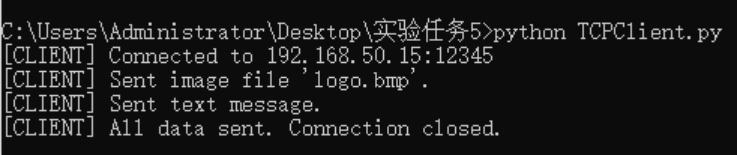
\includegraphics[width=\textwidth]{images/81.jpg}
        \caption{H1客户端成功连接服务器并发送了图片和文字数据后，正常关闭连接。}
    \end{figure}

    \item \textbf{H5 (服务器端) 输出}：
    \begin{figure}[H]
        \centering
        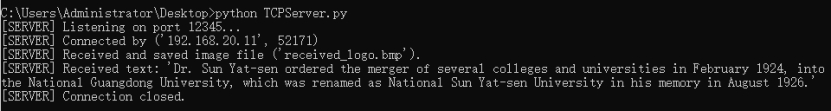
\includegraphics[width=\textwidth]{images/82.jpg}
        \caption{H5服务器端成功接收到来自H1的连接，并正确解析、保存了图片文件，同时打印出了接收到的完整文字信息。}
    \end{figure}
\end{itemize}

\textbf{数据完整性验证}：

1. \textbf{文字内容比对}：通过肉眼观察图82中服务器打印的文字，可以确认其内容与客户端代码中定义的\texttt{text\_message}完全一致，无任何字符丢失或错乱。

2. \textbf{图片文件验证}：

   \begin{itemize}
       \item 在 H5 的程序目录下，确认生成了名为 \texttt{received\_logo.bmp} 的图片文件，且可以正常打开。
       \begin{figure}[H]
           \centering
           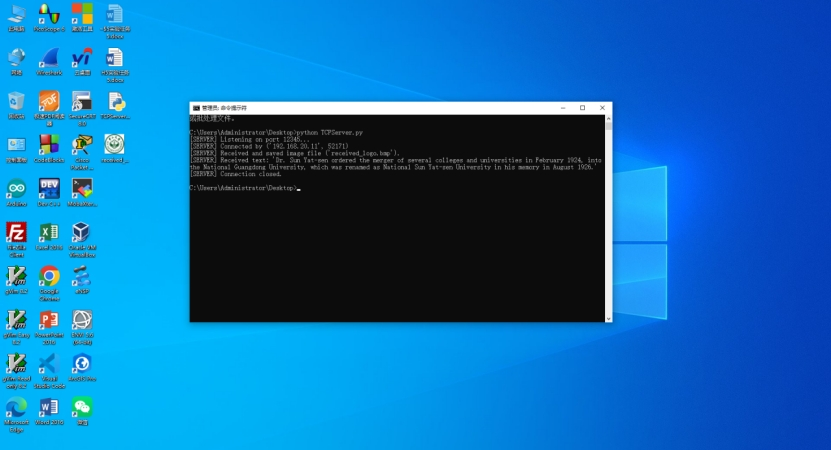
\includegraphics[width=\textwidth]{images/83.jpg}
           \caption{在H5上接收并保存的图片文件，可以正常预览。}
       \end{figure}

       \item 为了进行精确的、二进制级别的比对，我们分别在H1和H5上使用 \texttt{certutil -hashfile <文件名> MD5} 命令计算原始图片和接收图片的MD5哈希值。MD5是一种广泛使用的密码散列函数，能将任意长度的“字节串”变换成一个128位的大整数。如果两个文件的MD5值相同，就可以高度确信这两个文件内容完全一致。
       
       \begin{figure}[H]
           \centering
           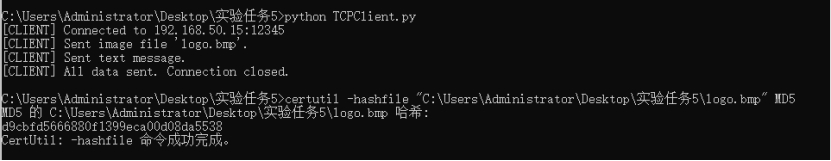
\includegraphics[width=\textwidth]{images/84.jpg}
           \caption{H1上原始文件 `logo.bmp` 的MD5哈希值。}
       \end{figure}

       \begin{figure}[H]
           \centering
           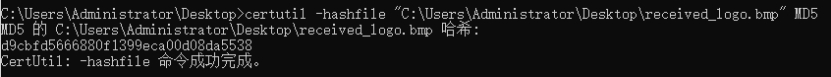
\includegraphics[width=\textwidth]{images/85.jpg}
           \caption{H5上接收文件 `received\_logo.bmp` 的MD5哈希值。}
       \end{figure}
   \end{itemize}

\textbf{结果分析}：如图84和图85所示，两个文件的MD5哈希值均为 \texttt{d9cbfd5666880f1399eca00d08da5538}，完全相同。这一结果验证了 TCP 协议的可靠性，表明图像文件在经过复杂的网络路径传输后，数据保持了完整性。

\textbf{结论}：本次传输实验成功地验证了TCP协议的可靠性。无论是结构化的文本数据还是非结构化的二进制文件数据，TCP的内在机制（如三次握手、序列号与确认、数据校验、超时重传、流量控制等）都确保了数据能够准确无误地从发送端送达接收端。

\subsection{传输路径抓包深度分析}

\subsubsection{H1 (发送端)：TCP流的起点}

\begin{figure}[H]
    \centering
    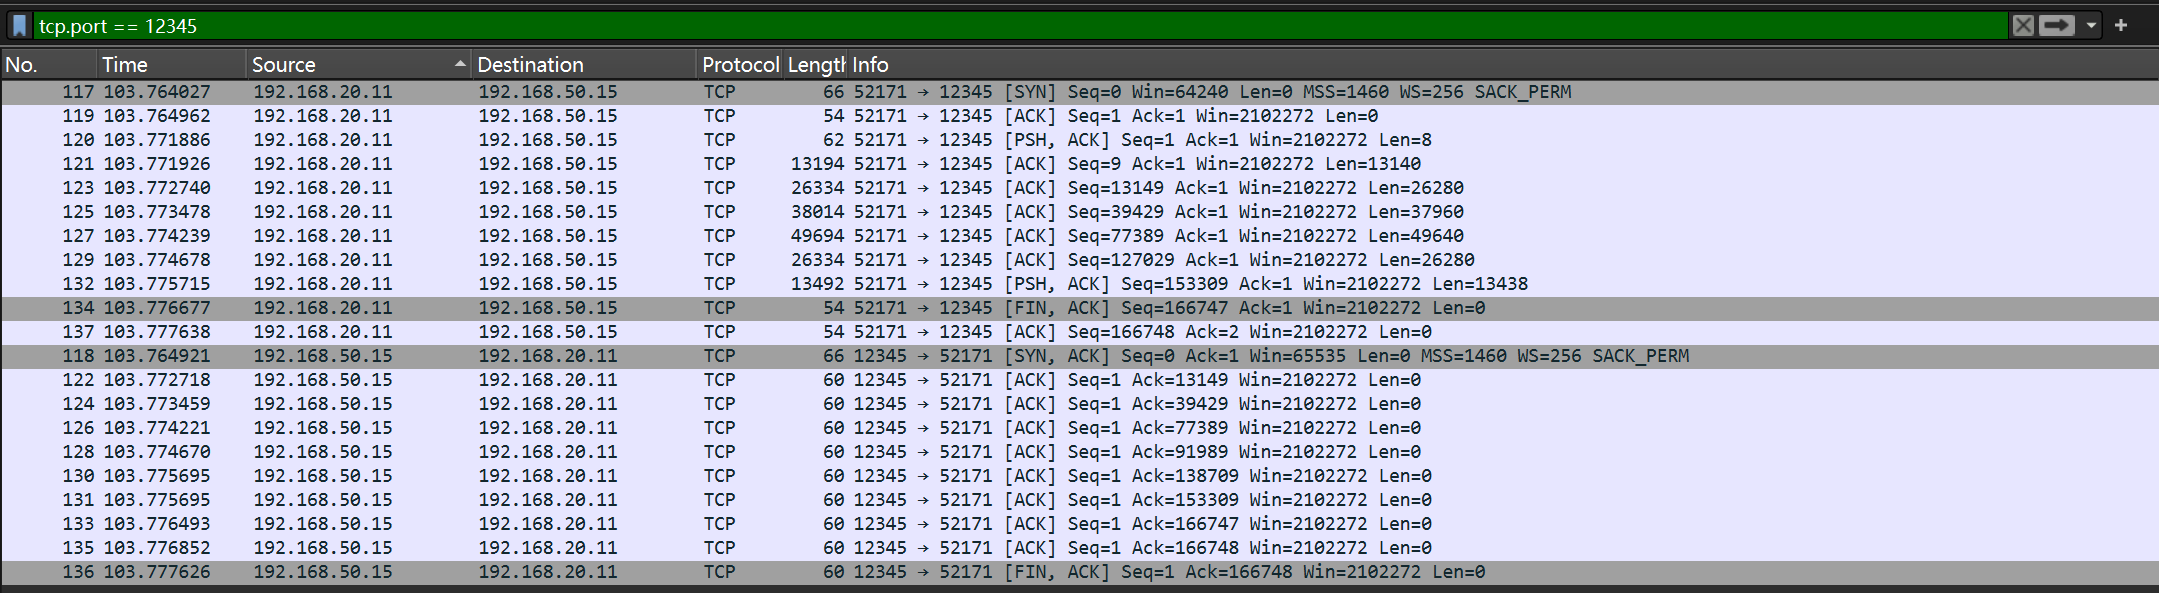
\includegraphics[width=\textwidth]{images/87.png}
    \caption{在H1上捕获的TCP通信全过程，包括三次握手、数据传输和四次挥手。}
\end{figure}

\textbf{分析}：

\begin{itemize}
    \item \textbf{TCP 连接建立（三次握手）}：
    抓包中前3个包（编号117、118、119）清晰地展示了标准的TCP三次握手过程，用于建立与H5的可靠连接：
    \begin{enumerate}
        \item \textbf{包 117}：H1$\rightarrow$H5 的 \textbf{SYN} 包（\texttt{Seq=0}），这是客户端H1发起的连接请求。其中包含了重要的协商参数，如\texttt{MSS=1460}（最大报文段大小）和窗口缩放因子等，为后续高效数据传输奠定基础。
        \item \textbf{包 118}：H5$\rightarrow$H1 的 \textbf{SYN+ACK} 包（\texttt{Seq=0, Ack=1}），这是服务器H5对H1请求的响应，表示同意建立连接，并同时发起自己的同步请求。
        \item \textbf{包 119}：H1$\rightarrow$H5 的 \textbf{ACK} 包（\texttt{Seq=1, Ack=1}），这是客户端H1对服务器响应的最终确认。至此，三次握手完成，一条全双工的TCP连接正式建立。
    \end{enumerate}
    
    \item \textbf{数据传输 (包120及之后)}：
    \begin{itemize}
        \item \textbf{包120} 是一个长度为8字节的PSH+ACK包，这正是我们自定义的应用层协议头部(type=1表示图片、len=166518表示图片总大小)。
        \item \textbf{包121} 开始是长度为13140字节的TCP段，Wireshark的\texttt{Len}字段显示的是TCP负载长度。实际上，IP层会将这个大的TCP段分割成多个IP包进行传输，每个IP包的数据部分（TCP段）不超过MSS（1460字节）。
        \item \textbf{包122、124 等} 是H5向H1返回ACK，H5 向 H1 返回 ACK，确认已接收的数据（如包 122 的 Ack=13149，对应包 121 的 Seq+Len）。
        \item \textbf{TCP流追踪}：为了更直观地看到应用层数据，我们使用Wireshark的“追踪TCP流”功能。
    \end{itemize}
\end{itemize}

\begin{figure}[H]
    \centering
    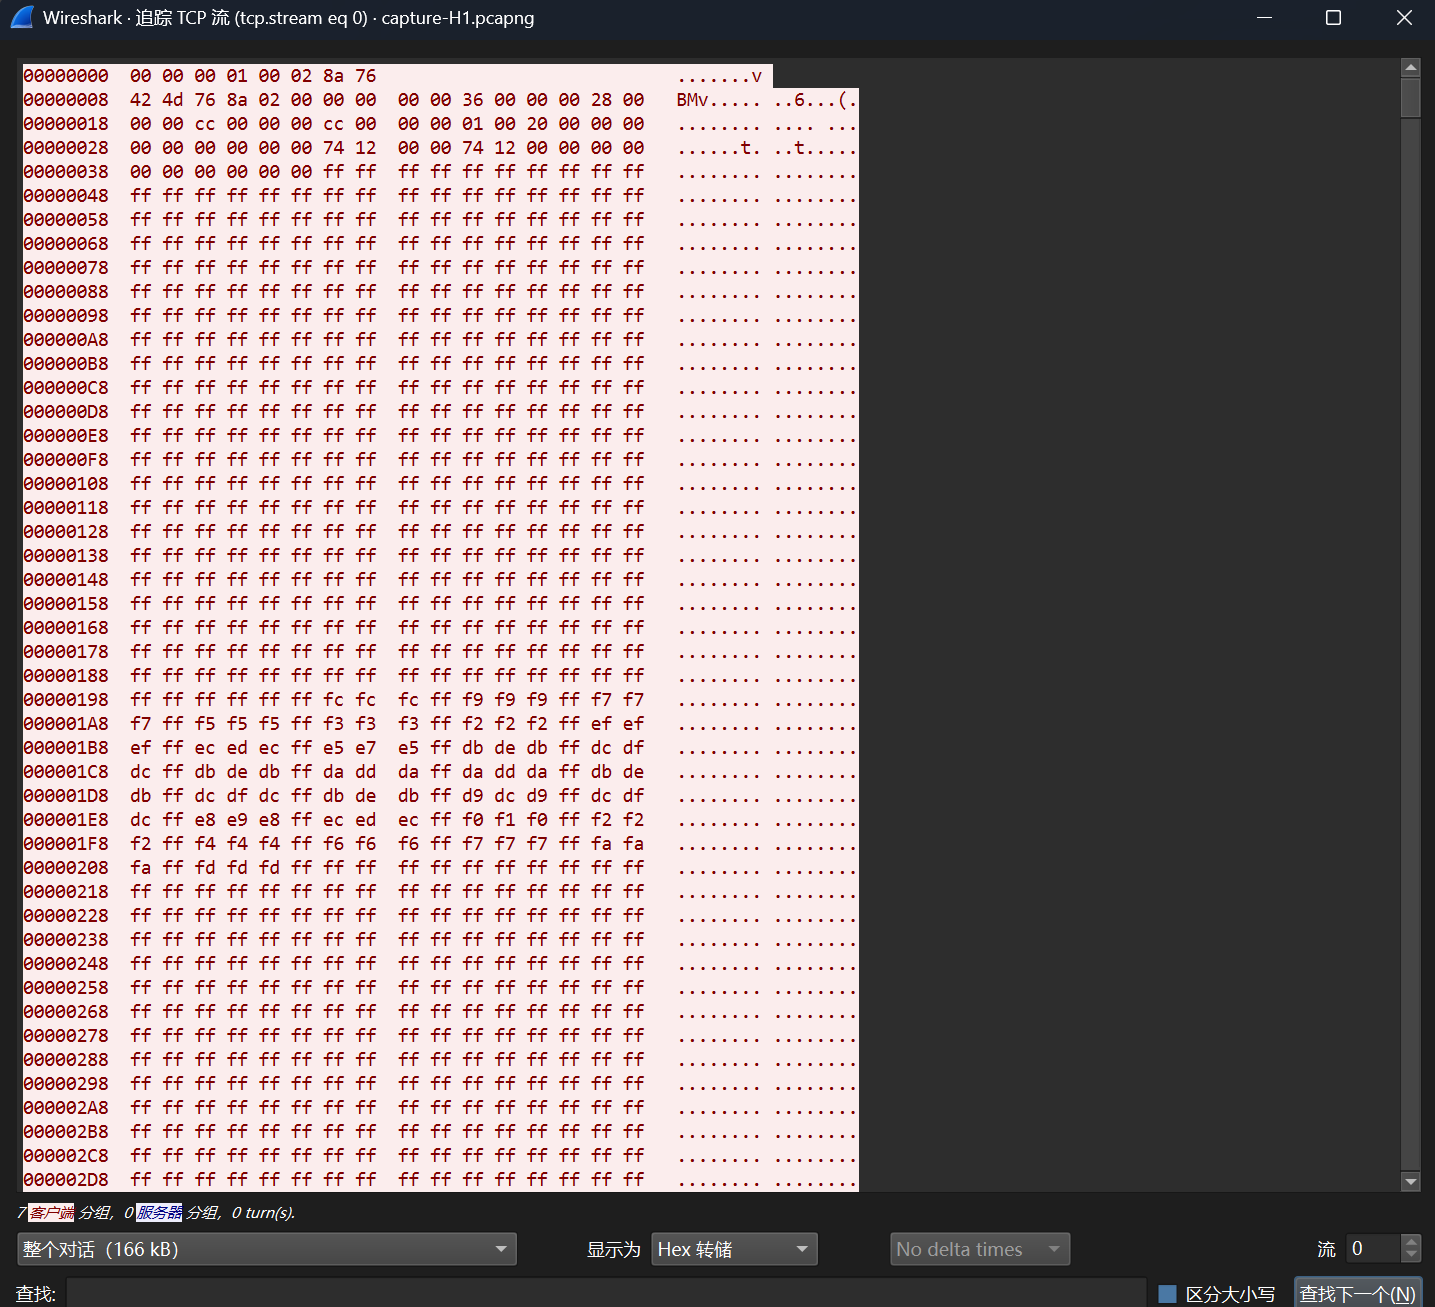
\includegraphics[width=\textwidth]{images/88.png}
    \caption{H1发送的TCP流内容，清晰可见自定义头部、BMP文件头和英文文本。}
\end{figure}

\textbf{TCP流内容分析}：

\begin{enumerate}
    \item \textbf{自定义应用层头部（8 字节）}：在TCP流的起始位置（偏移\texttt{0x00000000}），我们看到了\texttt{00 00 00 01 00 02 8A 76}这8个字节。这与我们Python代码中定义的“8字节头（类型+长度）”协议完全吻合。
    \begin{itemize}
        \item 前4字节 \texttt{00 00 00 01} $\rightarrow$ 按 \texttt{!I}（网络字节序）解包，得到 \texttt{data\_type = 1}，代表\textbf{图片}。
        \item 后4字节 \texttt{00 02 8A 76} $\rightarrow$ 按 \texttt{!I} 解包，得到 \texttt{data\_len = 166,518} 字节，这与\texttt{logo.bmp}的文件大小完全一致。
    \end{itemize}
    \item \textbf{BMP 文件签名（Magic Number）}：紧接着自定义头部之后（偏移\texttt{0x00000008}），出现了\texttt{42 4D}，其ASCII码正是 \textbf{\texttt{"BM"}}。这是Windows BMP格式文件最典型的文件头标识，它的出现证明了图片数据已经开始传输。
    \item \textbf{文字数据}：在TCP流的后半部分，我们可以清晰地看到ASCII文本内容：“Dr. Sun Yat-sen ordered...”，这与客户端代码中待发送的文字消息完全一致。
\end{enumerate}

\begin{figure}[H]
    \centering
    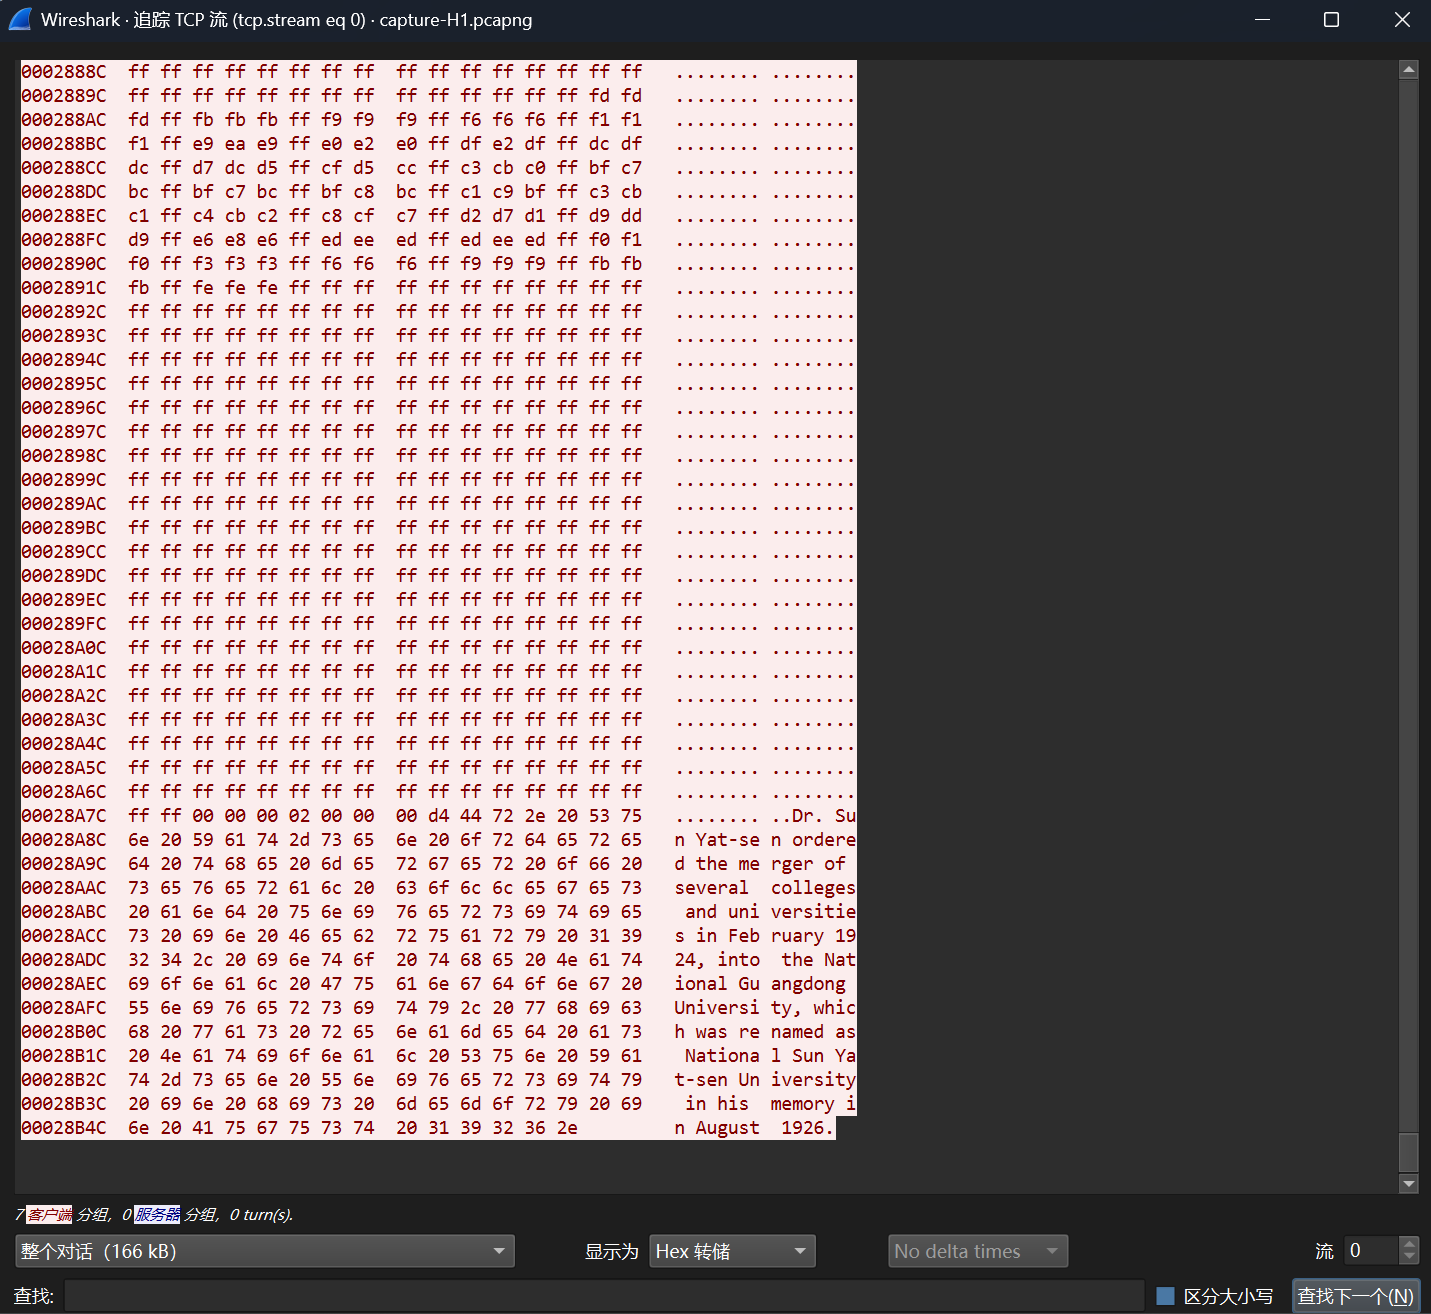
\includegraphics[width=\textwidth]{images/89.png}
    \caption{H1上捕获的数据包详细内容，显示了各层协议的头部信息。}
\end{figure}

\textbf{TCP 连接关闭（四次挥手）}：
在数据传输完毕后，抓包记录的末尾（包134、136、137）展示了标准的TCP四次挥手过程，用于优雅地关闭连接：

\begin{enumerate}
    \item \textbf{包 134}：H1$\rightarrow$H5 的 \texttt{FIN+ACK} 包，由客户端H1发起关闭请求。
    \item \textbf{包 136}：H5$\rightarrow$H1 的 \texttt{FIN+ACK} 包，服务器H5响应并同意关闭。
    \item \textbf{包 137}：H1$\rightarrow$H5 的 \texttt{ACK} 包，客户端H1对服务器的关闭请求进行最终确认，完成四次挥手。
\end{enumerate}

\textbf{小结}：在发送端H1，我们可以看到完整的TCP会话生命周期和清晰的应用层数据结构。此时的IP包初始TTL为128，源/目的IP和端口均已确定。

\subsubsection{交换机 S1 \& S2：二层透明转发}

数据包离开 H1 后，进入二层交换网络，依次经过交换机 S1 和 S2。我们在两台交换机上都配置了端口镜像，以观察数据包在纯二层转发环境下的状态。

\textbf{在交换机 S1 的抓包分析}

\begin{figure}[H]
    \centering
    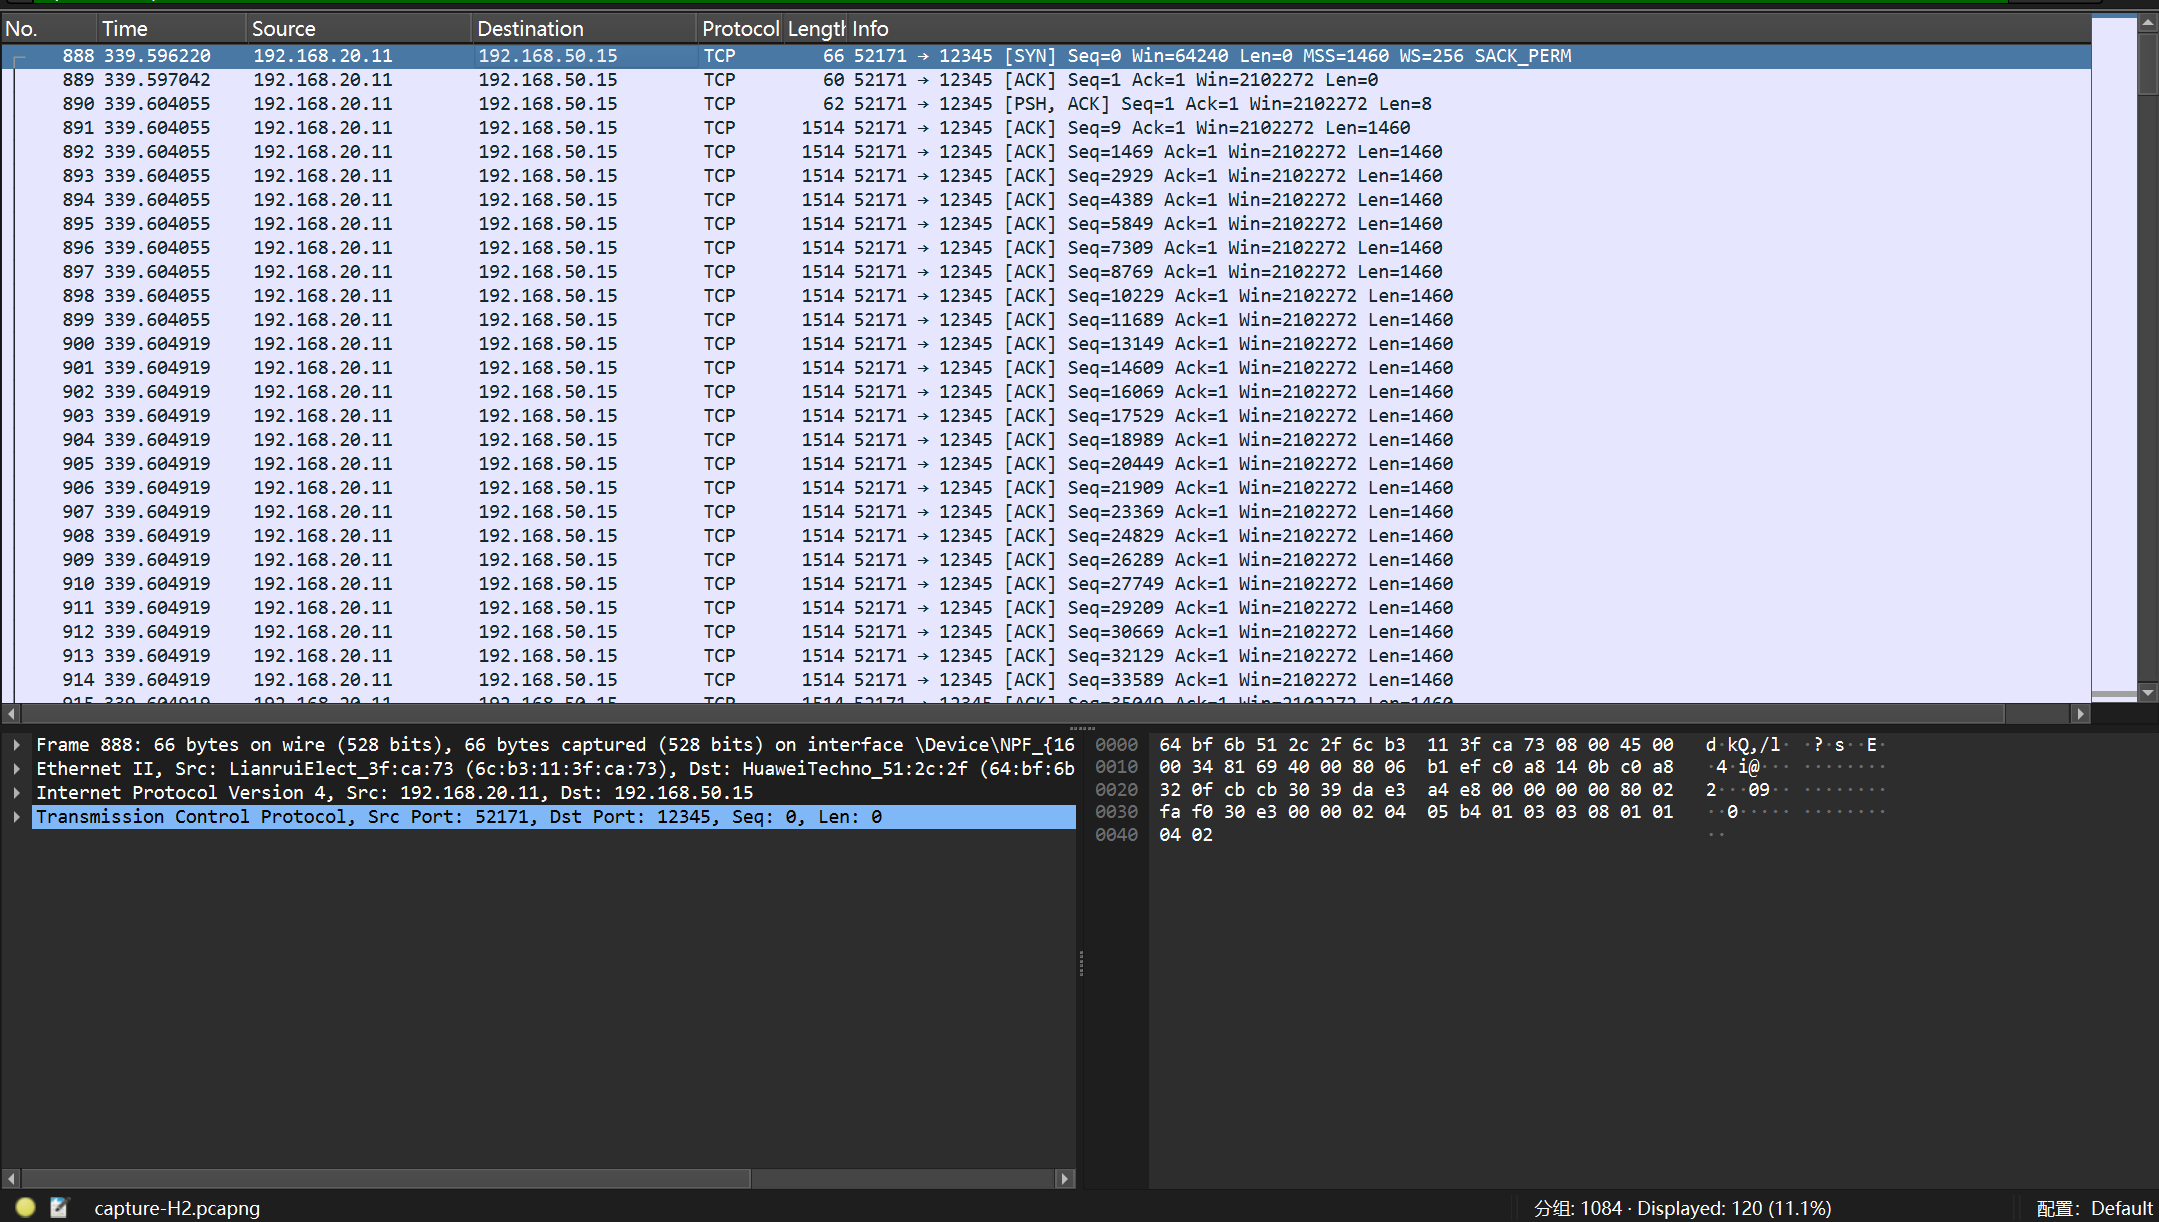
\includegraphics[width=\textwidth]{images/90.png}
    \caption{在H2上通过镜像S1端口捕获的数据包，可以看到完整的TCP会话流，从SYN握手到数据传输。}
\end{figure}

\textbf{关键数据包深度解析 (S1)}

我们选取了三个代表性的数据包进行逐层分析：三次握手的第一个包（SYN）、我们自定义协议的头部包（PSH, ACK）、以及第一个满载的数据包（ACK）。

\begin{itemize}
    \item \textbf{包 888：TCP连接请求 (SYN)}
    \begin{figure}[H]
        \centering
        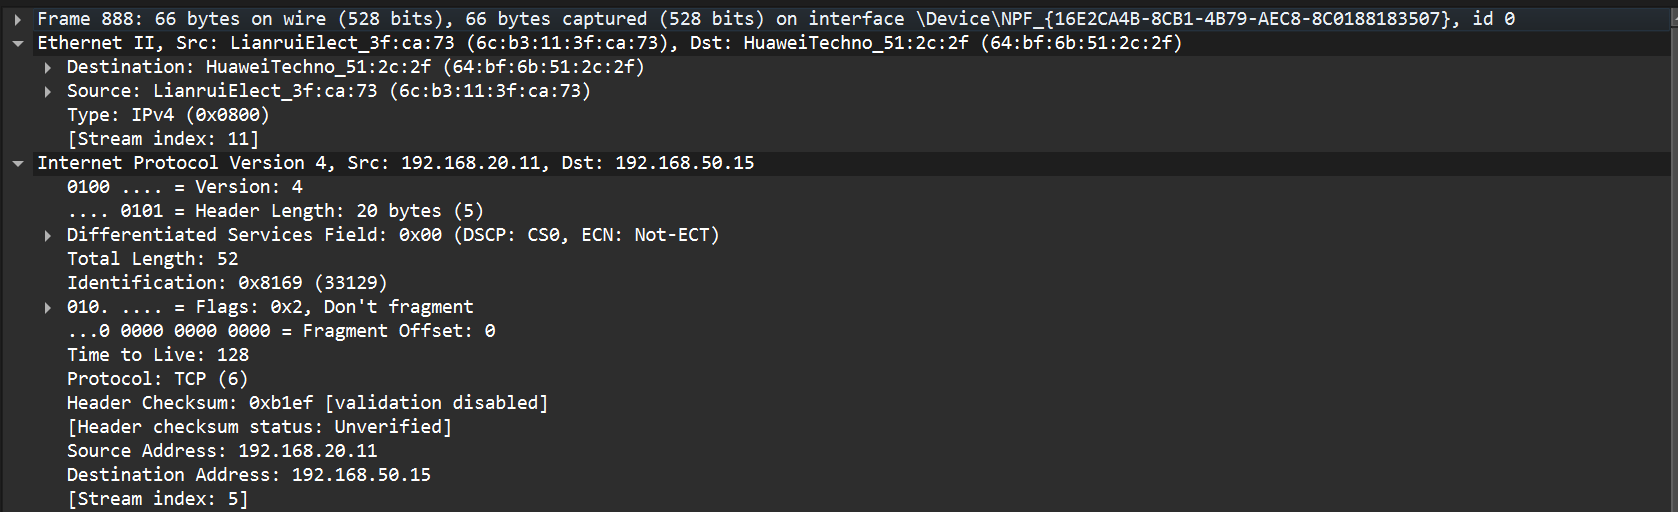
\includegraphics[width=\textwidth]{images/91.png}
        \caption{包 888 (SYN) 的数据链路层与网络层头部细节。}
    \end{figure}
    \begin{figure}[H]
        \centering
        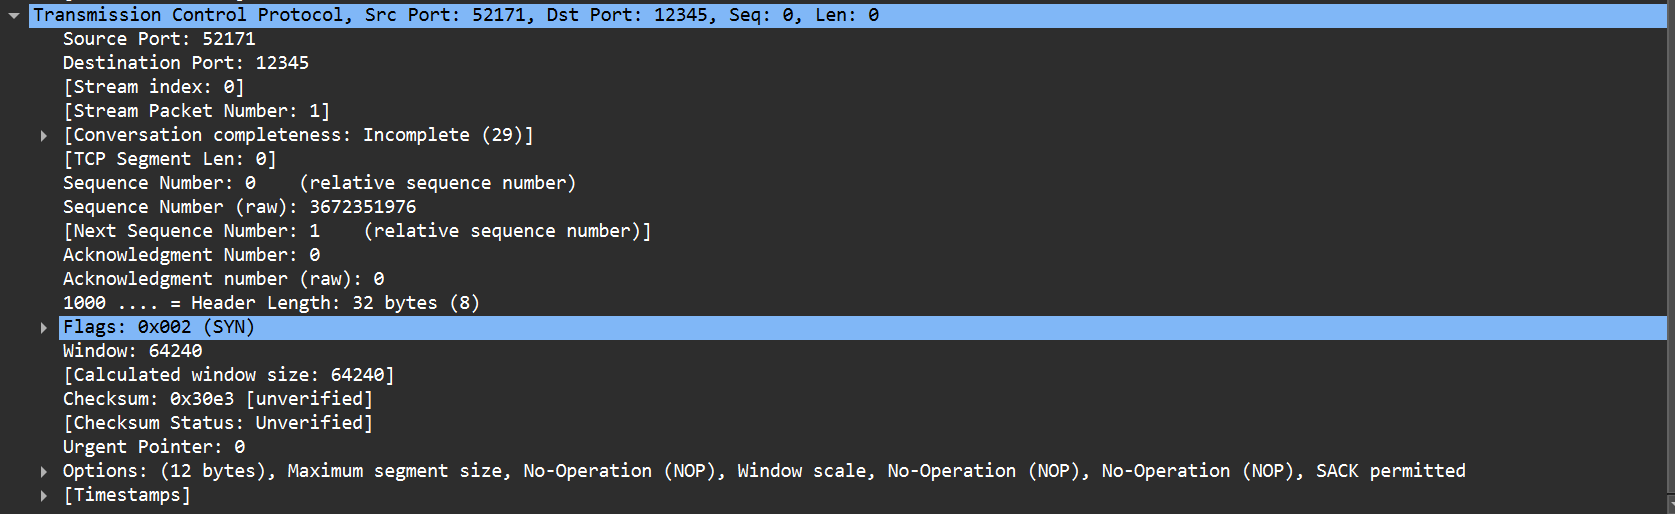
\includegraphics[width=\textwidth]{images/92.png}
        \caption{包 888 (SYN) 的传输层头部细节。}
    \end{figure}

    \textbf{分析}：
    \begin{itemize}
        \item \textbf{以太网层 (L2)}: 源MAC为 \texttt{6c:b3:11:3f:ca:73} (H1的物理地址)，目的MAC为 \texttt{64:bf:6b:51:2c:2f} (网关R1接口的物理地址)。
        \item \textbf{IPv4层 (L3)}: 源IP为 \texttt{192.168.20.11} (H1)，目的IP为 \texttt{192.168.50.15} (H5)。\textbf{TTL值为128}，这是Windows系统发包的初始值。
        \item \textbf{TCP层 (L4)}: 这是一个标准的SYN包，标志位\texttt{SYN}被置位，用于发起TCP连接。客户端通告其MSS为1460字节，并启用了窗口缩放(Window Scale)和选择性确认(SACK)选项。
    \end{itemize}

    \item \textbf{包 890：自定义协议头部传输 (PSH, ACK)}
    \begin{figure}[H]
        \centering
        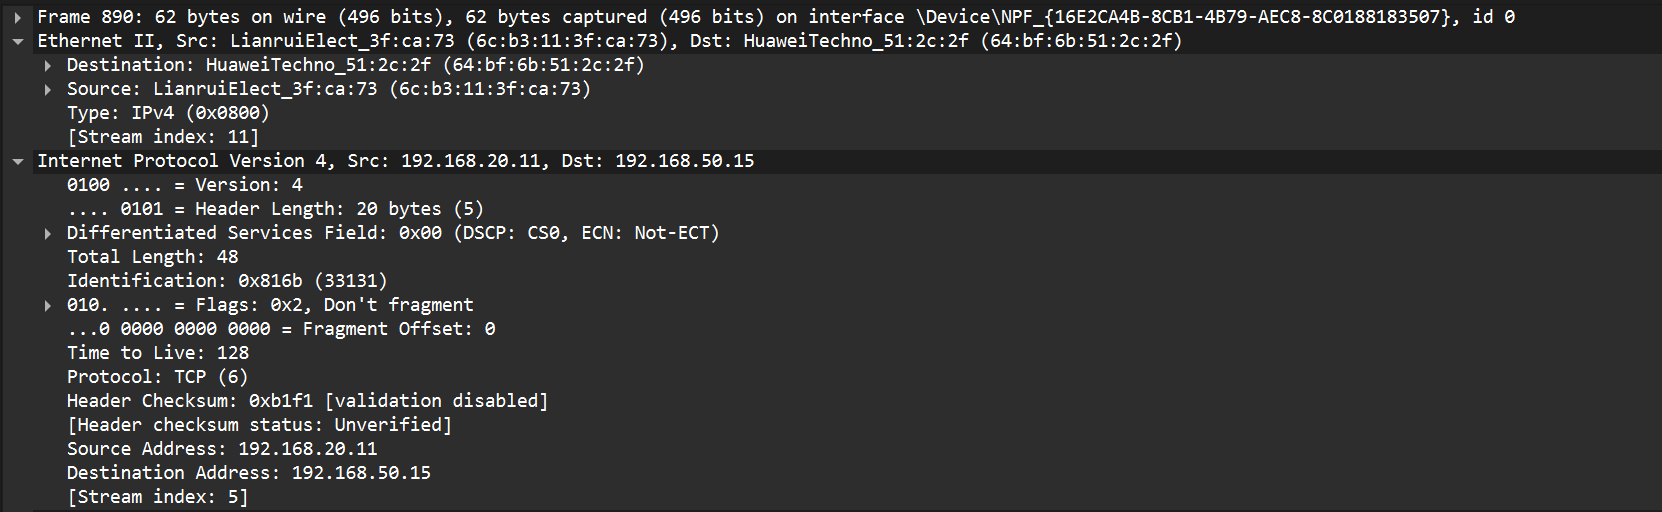
\includegraphics[width=\textwidth]{images/93.png}
        \caption{包 890 (PSH, ACK) 的二层与三层头部。}
    \end{figure}
    \begin{figure}[H]
        \centering
        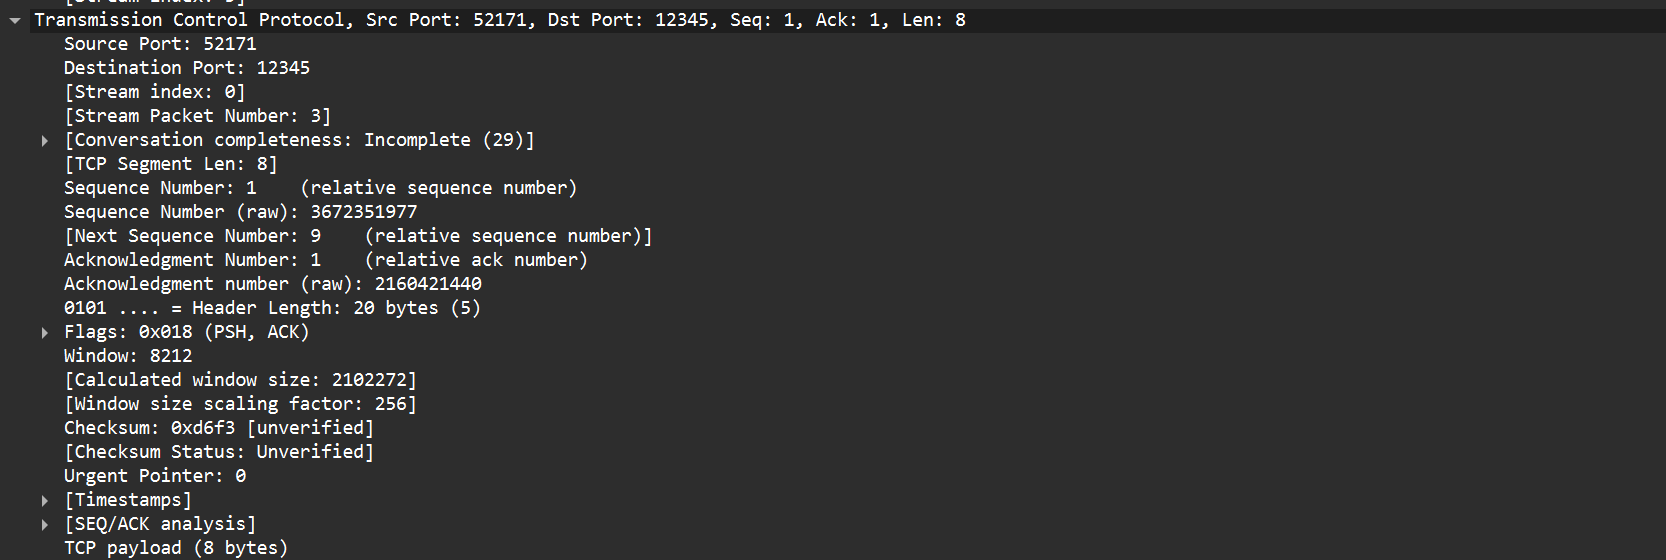
\includegraphics[width=\textwidth]{images/94.png}
        \caption{包 890 (PSH, ACK) 的传输层头部，可见数据载荷为8字节。}
    \end{figure}

    \textbf{分析}：
    \begin{itemize}
        \item L2和L3层的地址信息保持不变，TTL依然是128。
        \item \textbf{TCP层 (L4)}: 标志位为\texttt{PSH, ACK}，表示这是一个带有数据的确认包，且提示接收方应尽快将数据递交给应用层。其\textbf{数据长度(Len)为8字节}，这与我们代码中\texttt{struct.pack('!II', ...)}生成的8字节自定义头部完全吻合。
    \end{itemize}

    \item \textbf{包 891：首个满载数据段 (ACK)}
    \begin{figure}[H]
        \centering
        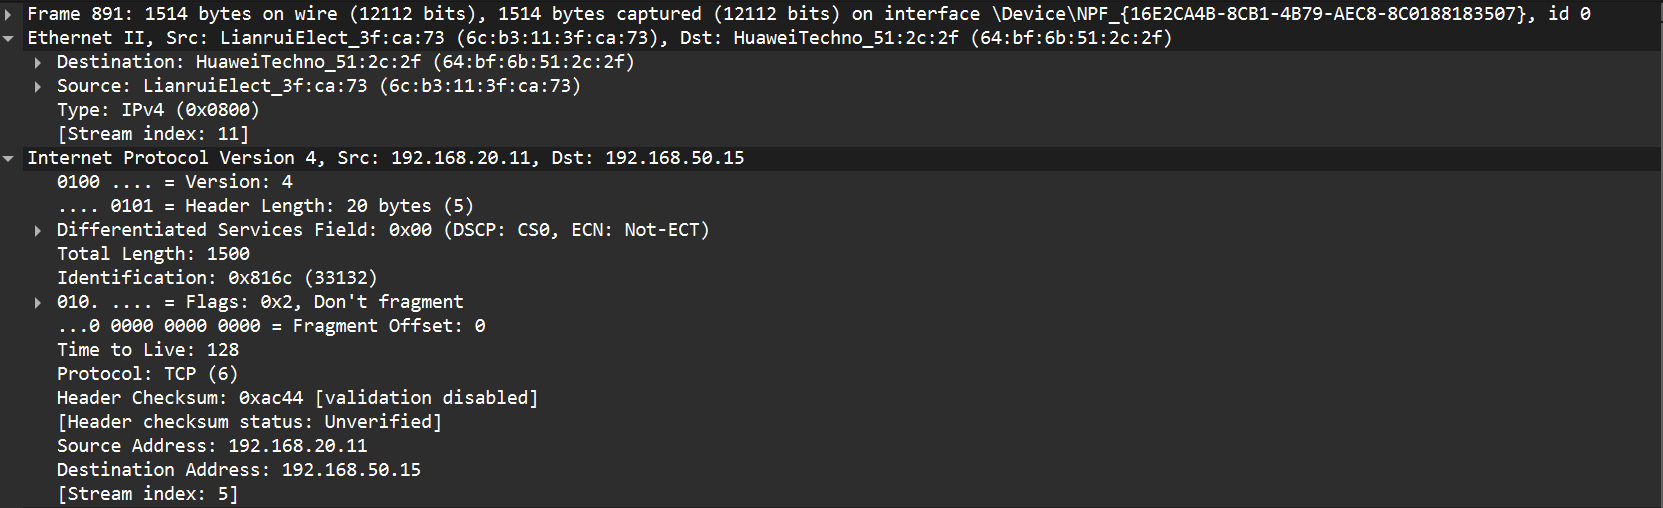
\includegraphics[width=\textwidth]{images/95.png}
        \caption{包 891 (ACK) 的二层与三层头部。}
    \end{figure}
    \begin{figure}[H]
        \centering
        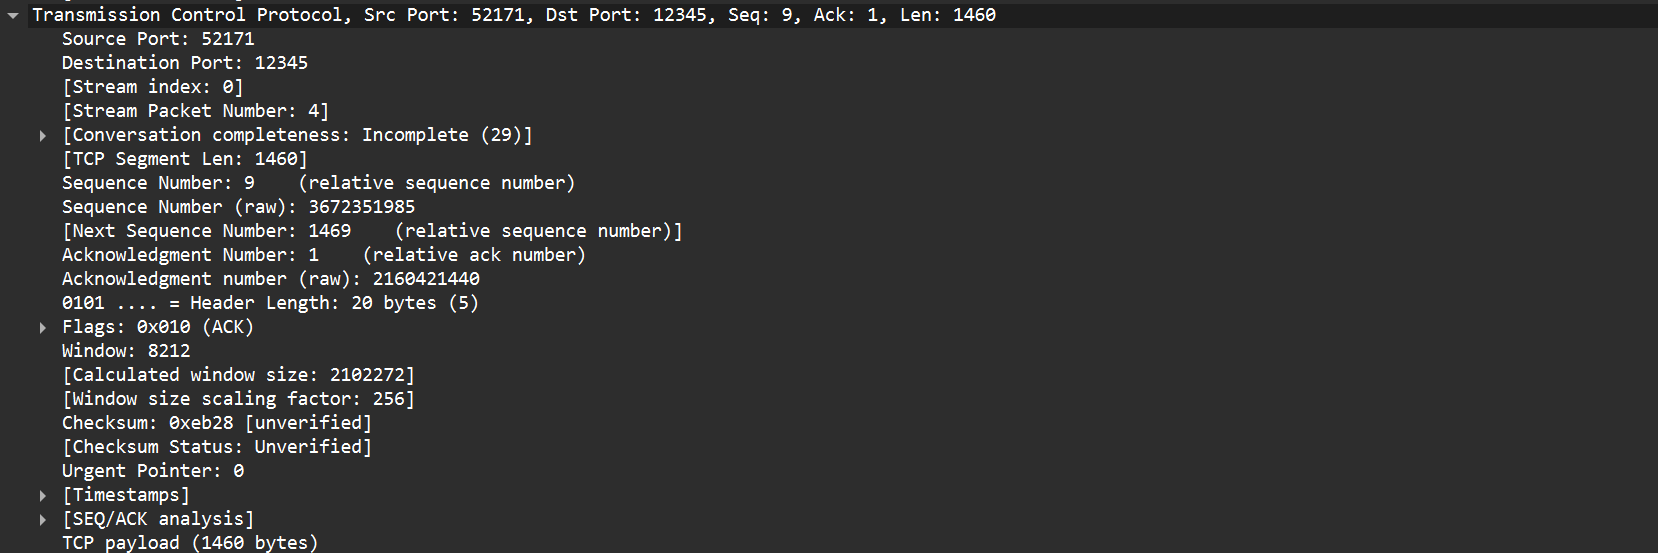
\includegraphics[width=\textwidth]{images/96.png}
        \caption{包 891 (ACK) 的传输层头部，数据载荷为1460字节。}
    \end{figure}

    \textbf{分析}：
    \begin{itemize}
        \item L2和L3层的地址信息和TTL值依然\textbf{保持不变}。
        \item \textbf{TCP层 (L4)}: 这是一个纯数据确认包（仅ACK标志位置位）。其\textbf{数据长度(Len)为1460字节}，这精确地等于三次握手时协商的MSS值，表明TCP协议正在以最高效率分片并传输我们的图片数据。
    \end{itemize}
\end{itemize}

\textbf{在交换机 S2 的抓包分析}

\begin{figure}[H]
    \centering
    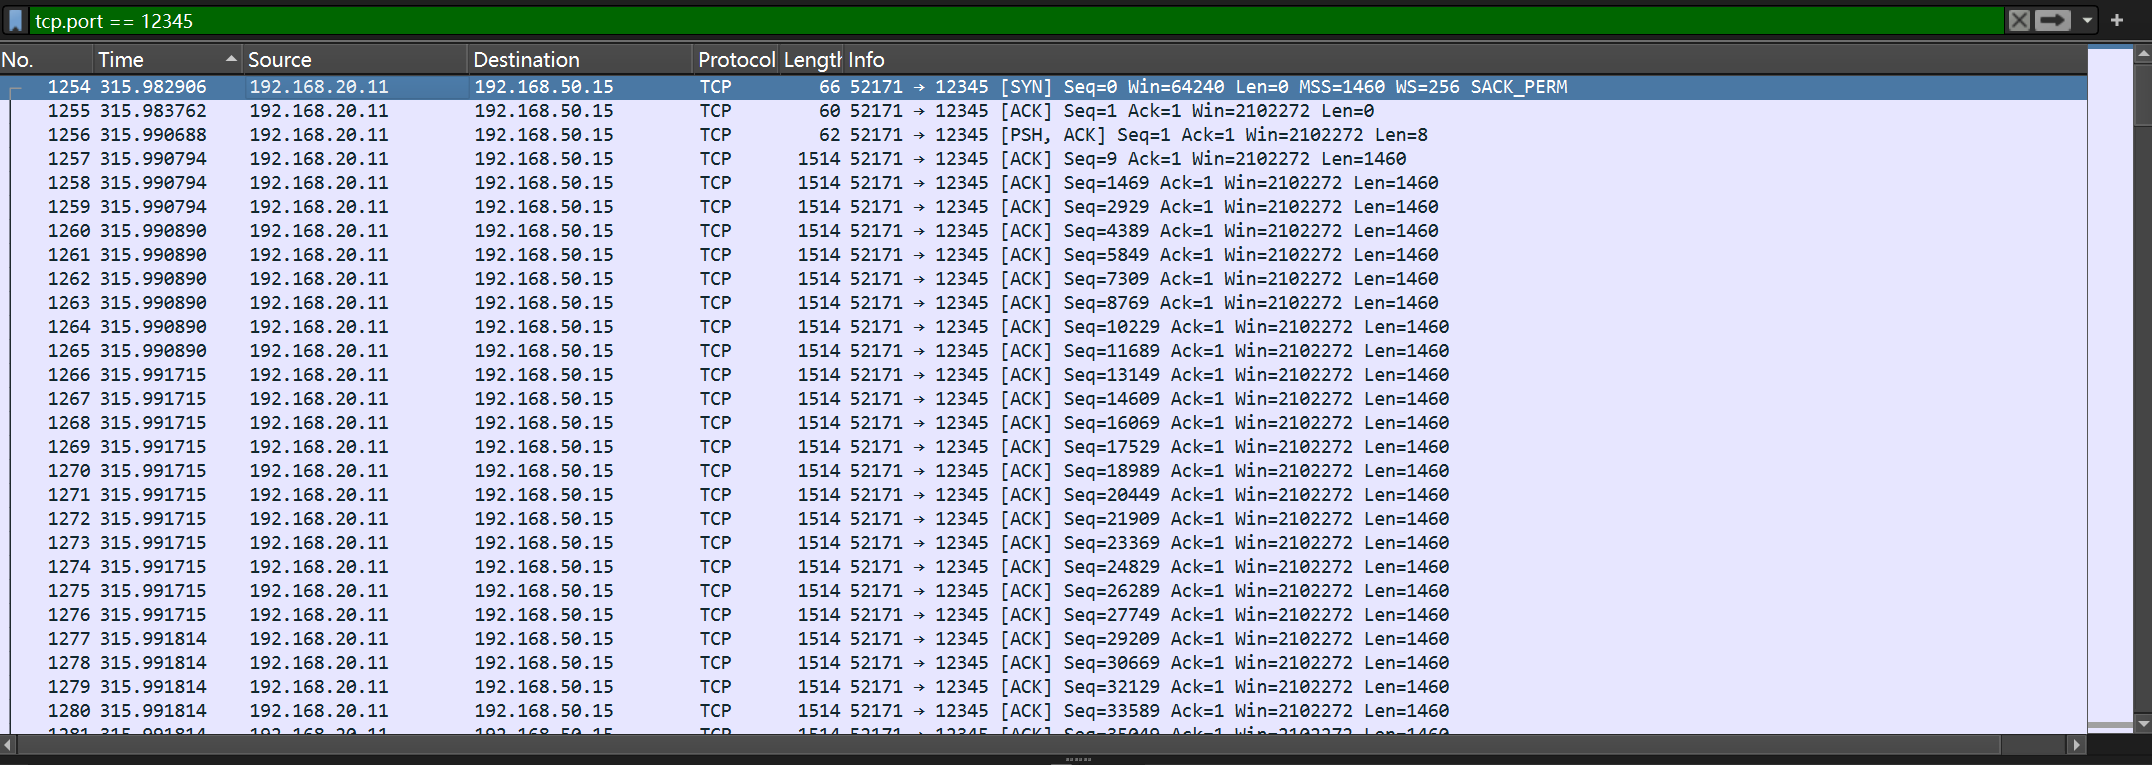
\includegraphics[width=\textwidth]{images/97.png}
    \caption{在H4上通过镜像S2端口捕获的数据包，其内容与S1抓包结果高度一致。}
\end{figure}

\begin{itemize}
    \item \textbf{关键数据包深度解析 (S2 - 包 1257，对应S1的包891)}
    \begin{figure}[H]
        \centering
        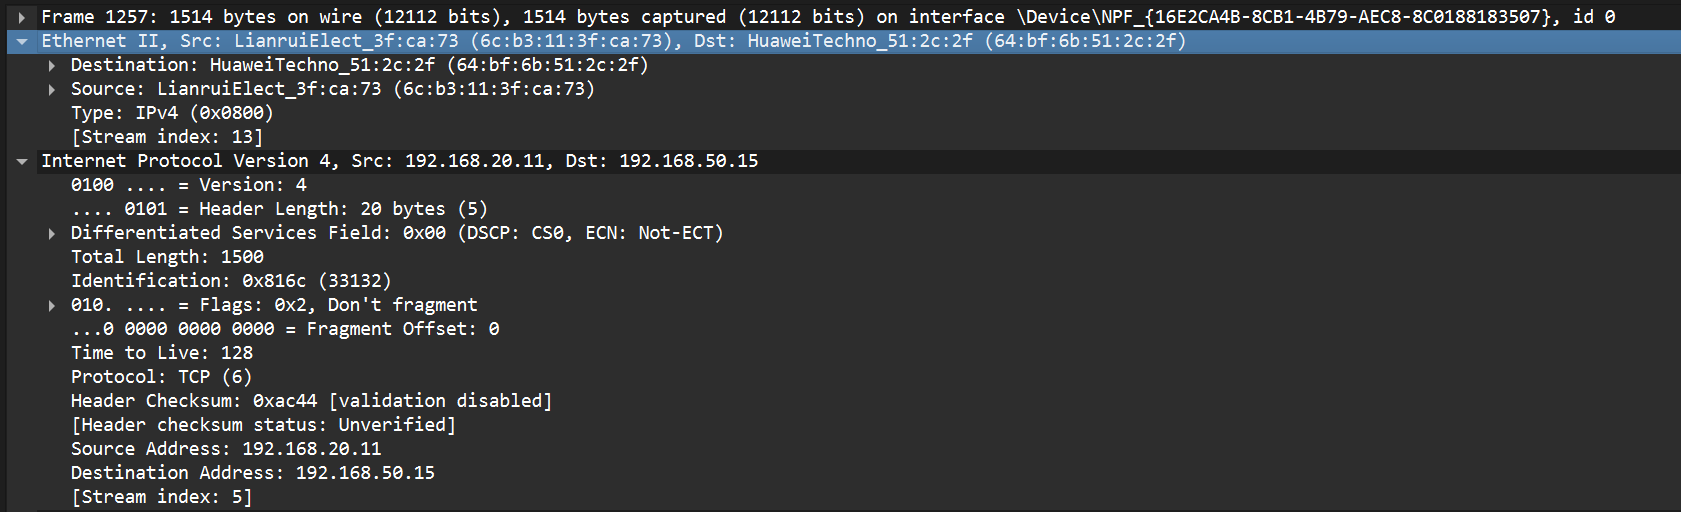
\includegraphics[width=\textwidth]{images/98.png}
        \caption{S2捕获的数据包二层与三层头部。}
    \end{figure}
    \begin{figure}[H]
        \centering
        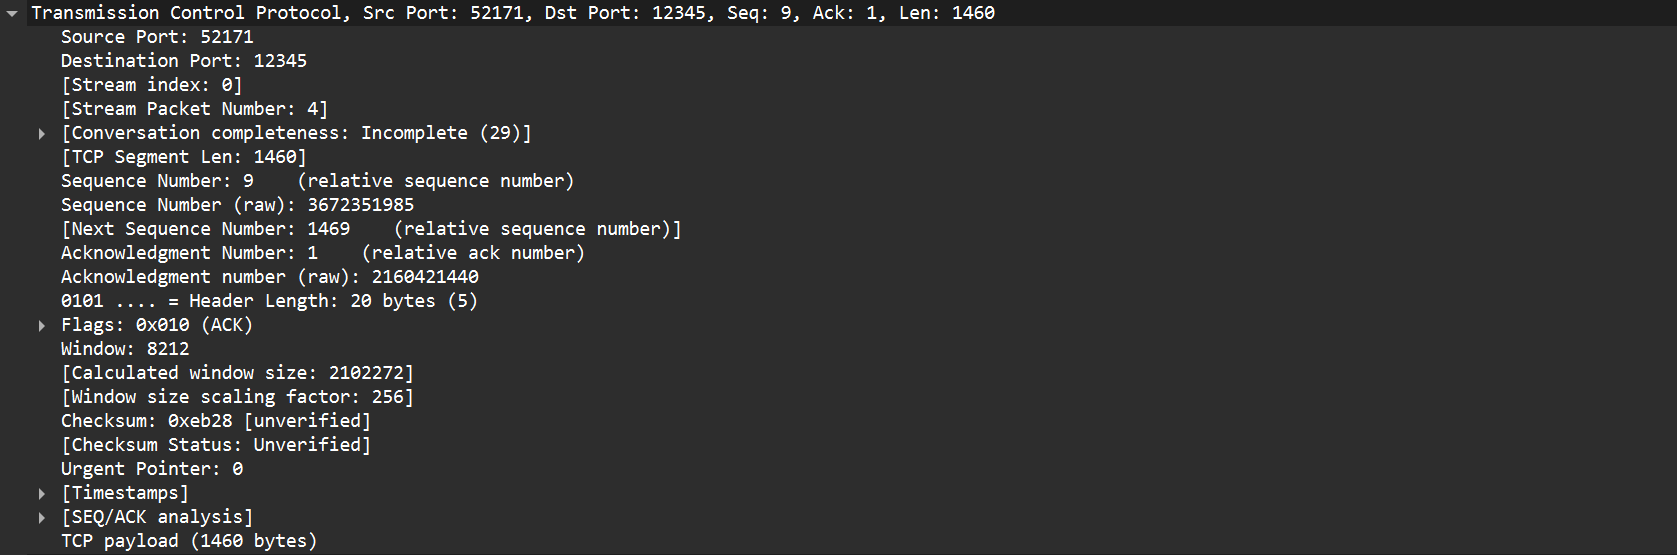
\includegraphics[width=\textwidth]{images/99.png}
        \caption{S2捕获的数据包传输层头部。}
    \end{figure}

    \textbf{分析}：通过对比S2捕获的包1257和S1捕获的包891，我们发现，从二层的MAC地址对，到三层的IP地址对和TTL值，再到四层的端口号、序列号和数据载荷，\textbf{所有字段都完全相同}。
\end{itemize}

\textbf{二层转发小结}
实验结果清晰地展示了交换机的工作原理：作为数据链路层（二层）设备，交换机仅根据以太网帧的目的MAC地址进行转发决策，它不会检查或修改帧内部封装的IP数据包。因此，数据包在跨越S1和S2的过程中，其内容（包括IP地址和TTL）保持了绝对的完整性。对于IP层而言，整个交换网络是一个透明的传输通道。

\subsubsection{路由器 R1：首次路由与重传现象}

数据包离开交换网络后，抵达其网关——路由器R1。这里是数据包第一次经历三层转发的地方。

\begin{figure}[H]
    \centering
    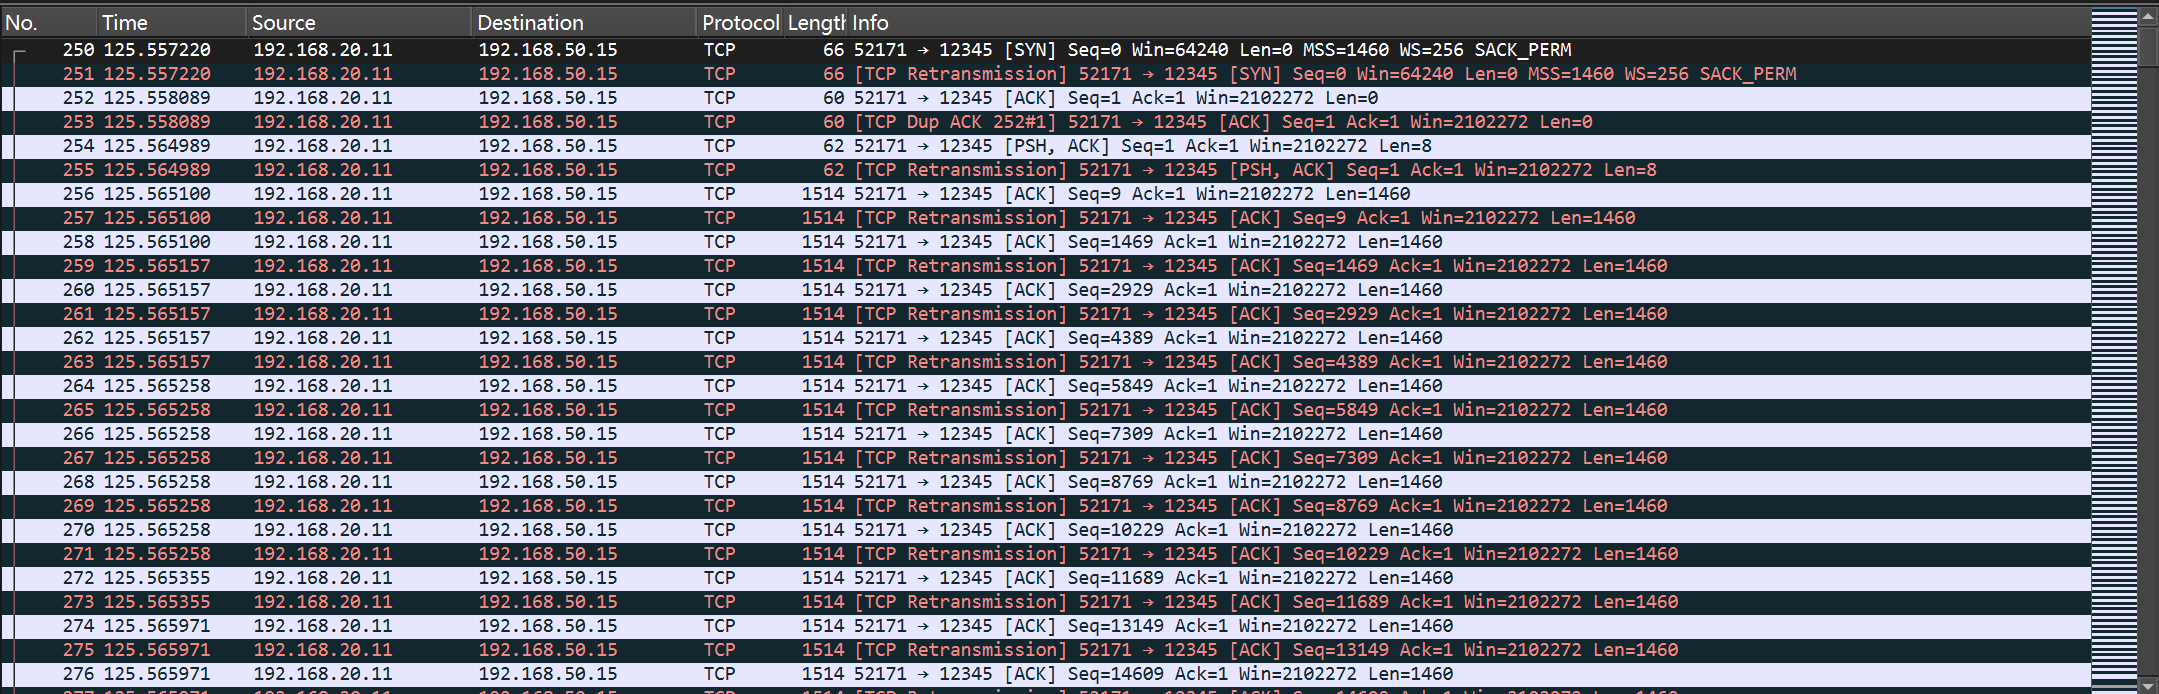
\includegraphics[width=\textwidth]{images/100.png}
    \caption{在H3上通过镜像R1端口捕获的数据包，一个显著的现象是出现了大量的TCP重传(TCP Retransmission)。}
\end{figure}

\textbf{现象分析：TCP重传}
在R1的抓包记录中，我们清晰地看到了TCP重传行为。这意味着发送端H1在发出了一个数据包后，未能在其动态计算的超时重传定时器（RTO）内收到来自H5的确认（ACK），因此它假定该数据包已丢失，并重新发送了完全相同的数据包。这恰好是TCP可靠性机制的核心体现。在我们的实验环境中，这可能是由于短时间内传输大文件导致下游链路（R1->R2->H5）出现瞬时拥塞或处理延迟，R1 作为中间转发节点，会将 H1 的数据包转发给 R2，但如果 R2 到 H5 的链路出现拥堵、丢包，或 H5 的接收缓冲区不足，会导致 H5 无法及时返回 ACK，最终使 H1 触发重传。这个现象为我们提供了一个观察真实网络中 TCP 协议动态调整行为的机会。

\begin{itemize}
    \item \textbf{关键数据包深度解析 (R1 - 包 250，SYN包)}
    \begin{figure}[H]
        \centering
        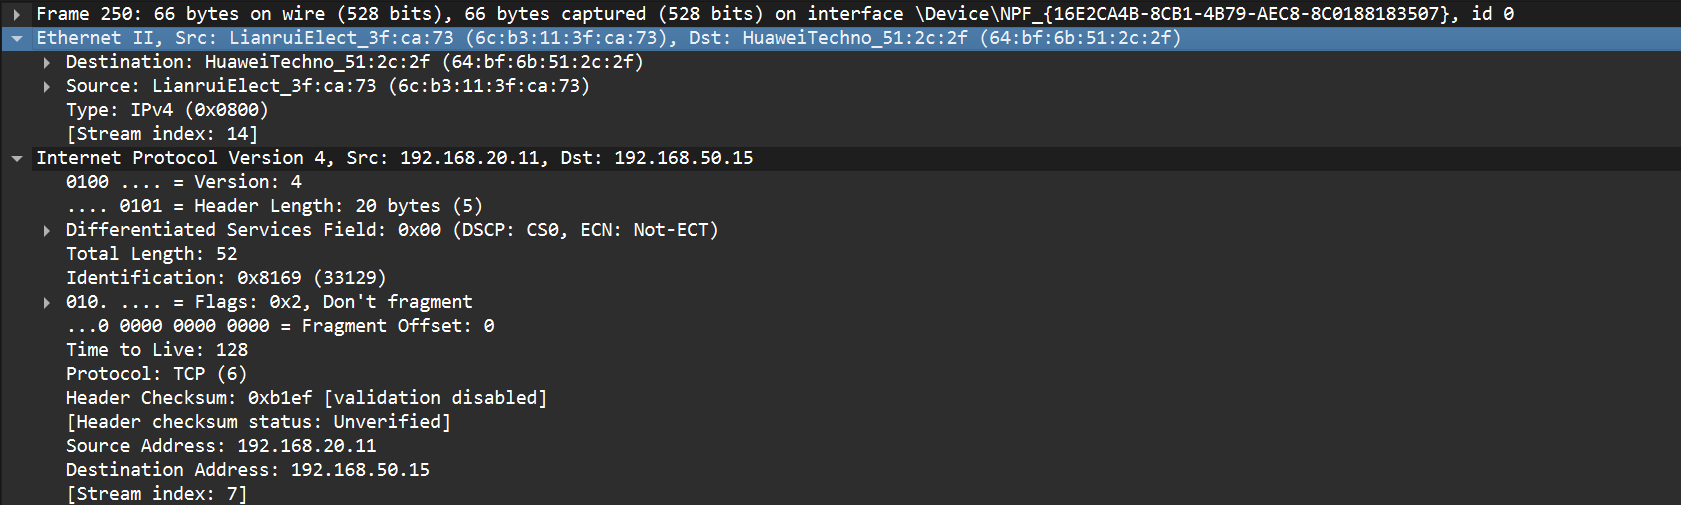
\includegraphics[width=\textwidth]{images/101.png}
        \caption{R1的入接口捕获的SYN包，其L2/L3头部与S1/S2处完全一致。}
    \end{figure}
    \begin{figure}[H]
        \centering
        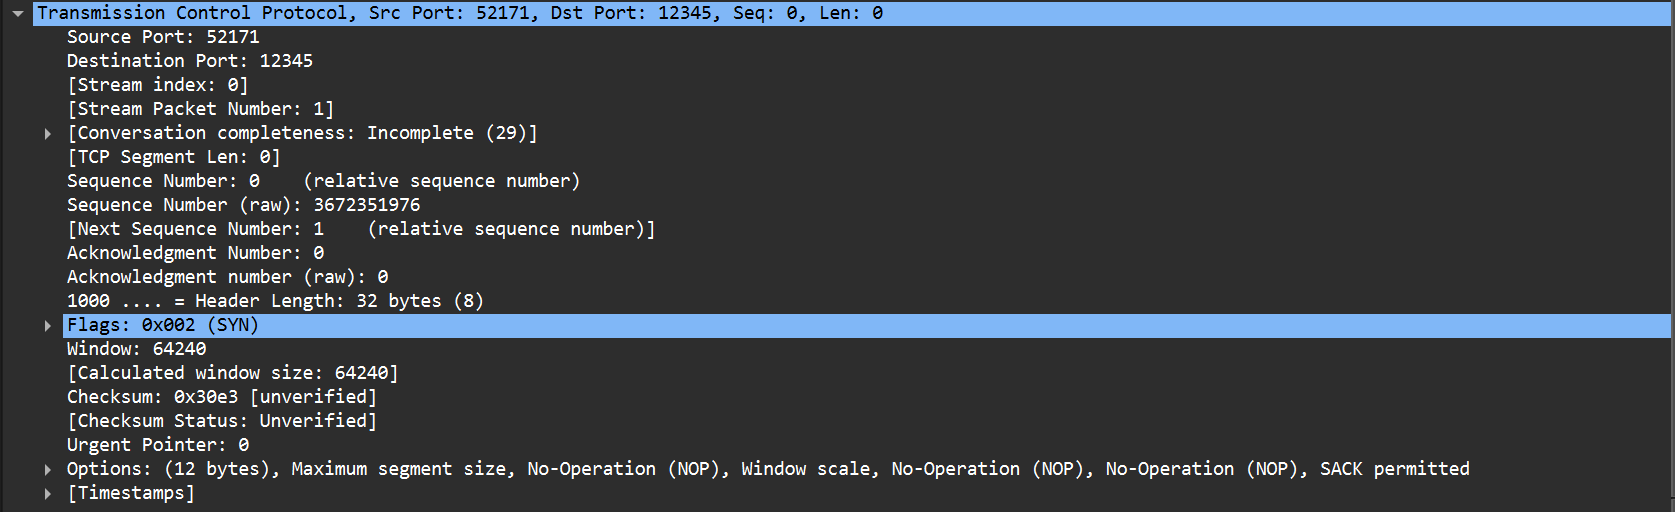
\includegraphics[width=\textwidth]{images/102.png}
        \caption{R1捕获的SYN包的传输层头部。}
    \end{figure}

    \textbf{分析}：这个数据包是在R1的\textbf{入接口}（GE0/0/2）捕获的，它代表了数据包刚刚从S2到达R1的状态。我们可以看到，此时此刻，数据包的所有头部信息（MAC地址、IP地址、TTL=128）与在S1和S2上看到的一模一样。\textbf{路由转发的关键动作发生在这个包被处理并从出接口发送出去之后}。
\end{itemize}

\subsubsection{路由器 R2：第二次路由与关键变化}

数据包经过R1的路由决策后，被转发至下一跳路由器R2。在R2的入接口抓包，是观察路由转发核心机制的最佳位置。

\begin{figure}[H]
    \centering
    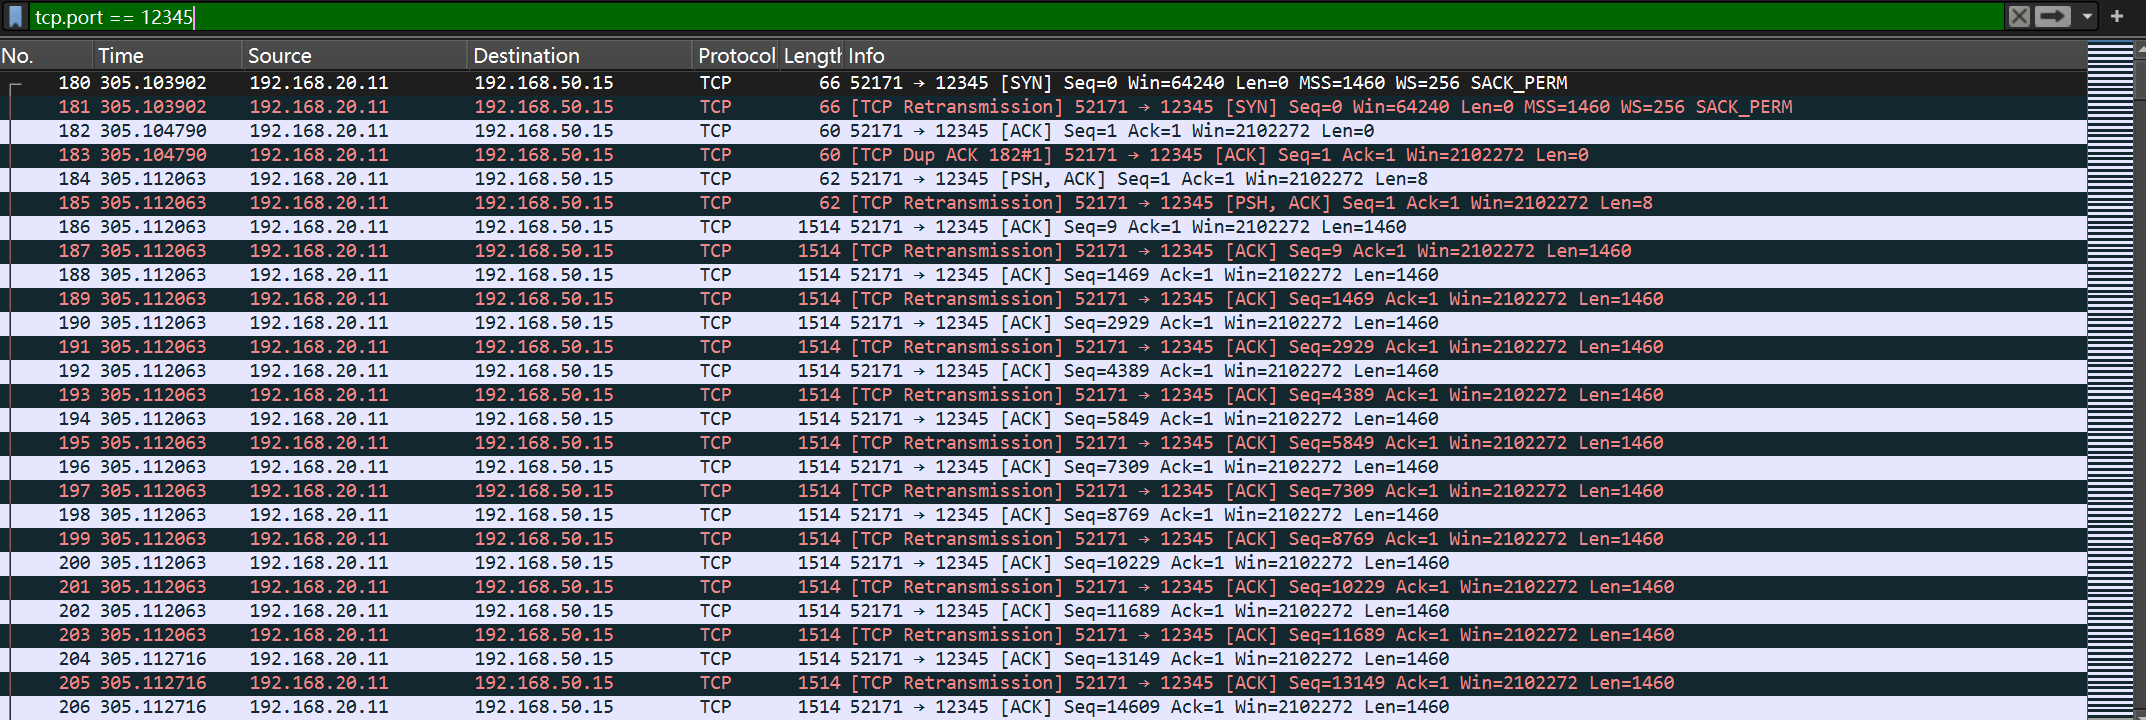
\includegraphics[width=\textwidth]{images/103.png}
    \caption{在H6上通过镜像R2端口捕获的数据包。}
\end{figure}

\textbf{关键数据包深度解析 (R2 - 包 180，SYN包)}

\textbf{分析}：包180是从R1发往R2的SYN包。我们将它的头部与之前在R1入接口看到的包250进行对比，发现了根本性的变化：

\begin{itemize}
    \item \textbf{以太网层 (L2) - 彻底重封装}:
    \begin{itemize}
        \item \textbf{源MAC地址}变为 \texttt{64:bf:6b:a8:b1:39}。这不再是H1的MAC，而是\textbf{路由器R1的出接口(GE0/0/0)的MAC地址}，同时因为与之前数据包的目的MAC地址同属一个路由器，故二者MAC地址前 \textbf{24 位（前 3 个字节，为OUI\textbf{组织唯一标识符} ）} 都是相同的 ，后 \textbf{24 位} 由厂商自行分配的设备 / 接口标识符完全不同。 
        \item \textbf{目的MAC地址}变为 \texttt{5c:e8:83:74:a4:24}。这不再是R1的MAC，而是\textbf{路由器R2的入接口(GE0/0/4)的MAC地址}。
        \item \textbf{结论}: 路由器\textbf{重写了整个以太网帧头}，以适配R1到R2这段新的数据链路。
    \end{itemize}
    
    \item \textbf{IPv4层 (L3) - TTL递减，IP不变}:
    \begin{itemize}
        \item \textbf{源IP和目的IP} 仍然是 \texttt{192.168.20.11} 和 \texttt{192.168.50.15}。IP地址作为端到端的逻辑地址，在路由过程中\textbf{保持不变}。
        \item \textbf{TTL (Time to Live)} 变为 \texttt{127}。该值在初始的128基础上\textbf{减了1}，因为IP包成功穿越了R1这个三层设备。这是防止路由环路的核心机制。
    \end{itemize}
    
    \item \textbf{TCP层 (L4)}: 传输层头部内容（端口号、序列号等）保持不变，路由器不关心也不修改四层信息。
\end{itemize}

\subsubsection{H5 (接收端)：TCP流的终点}

数据包经过R2的第二次路由转发后，最终抵达目的地H5。

\begin{figure}[H]
    \centering
    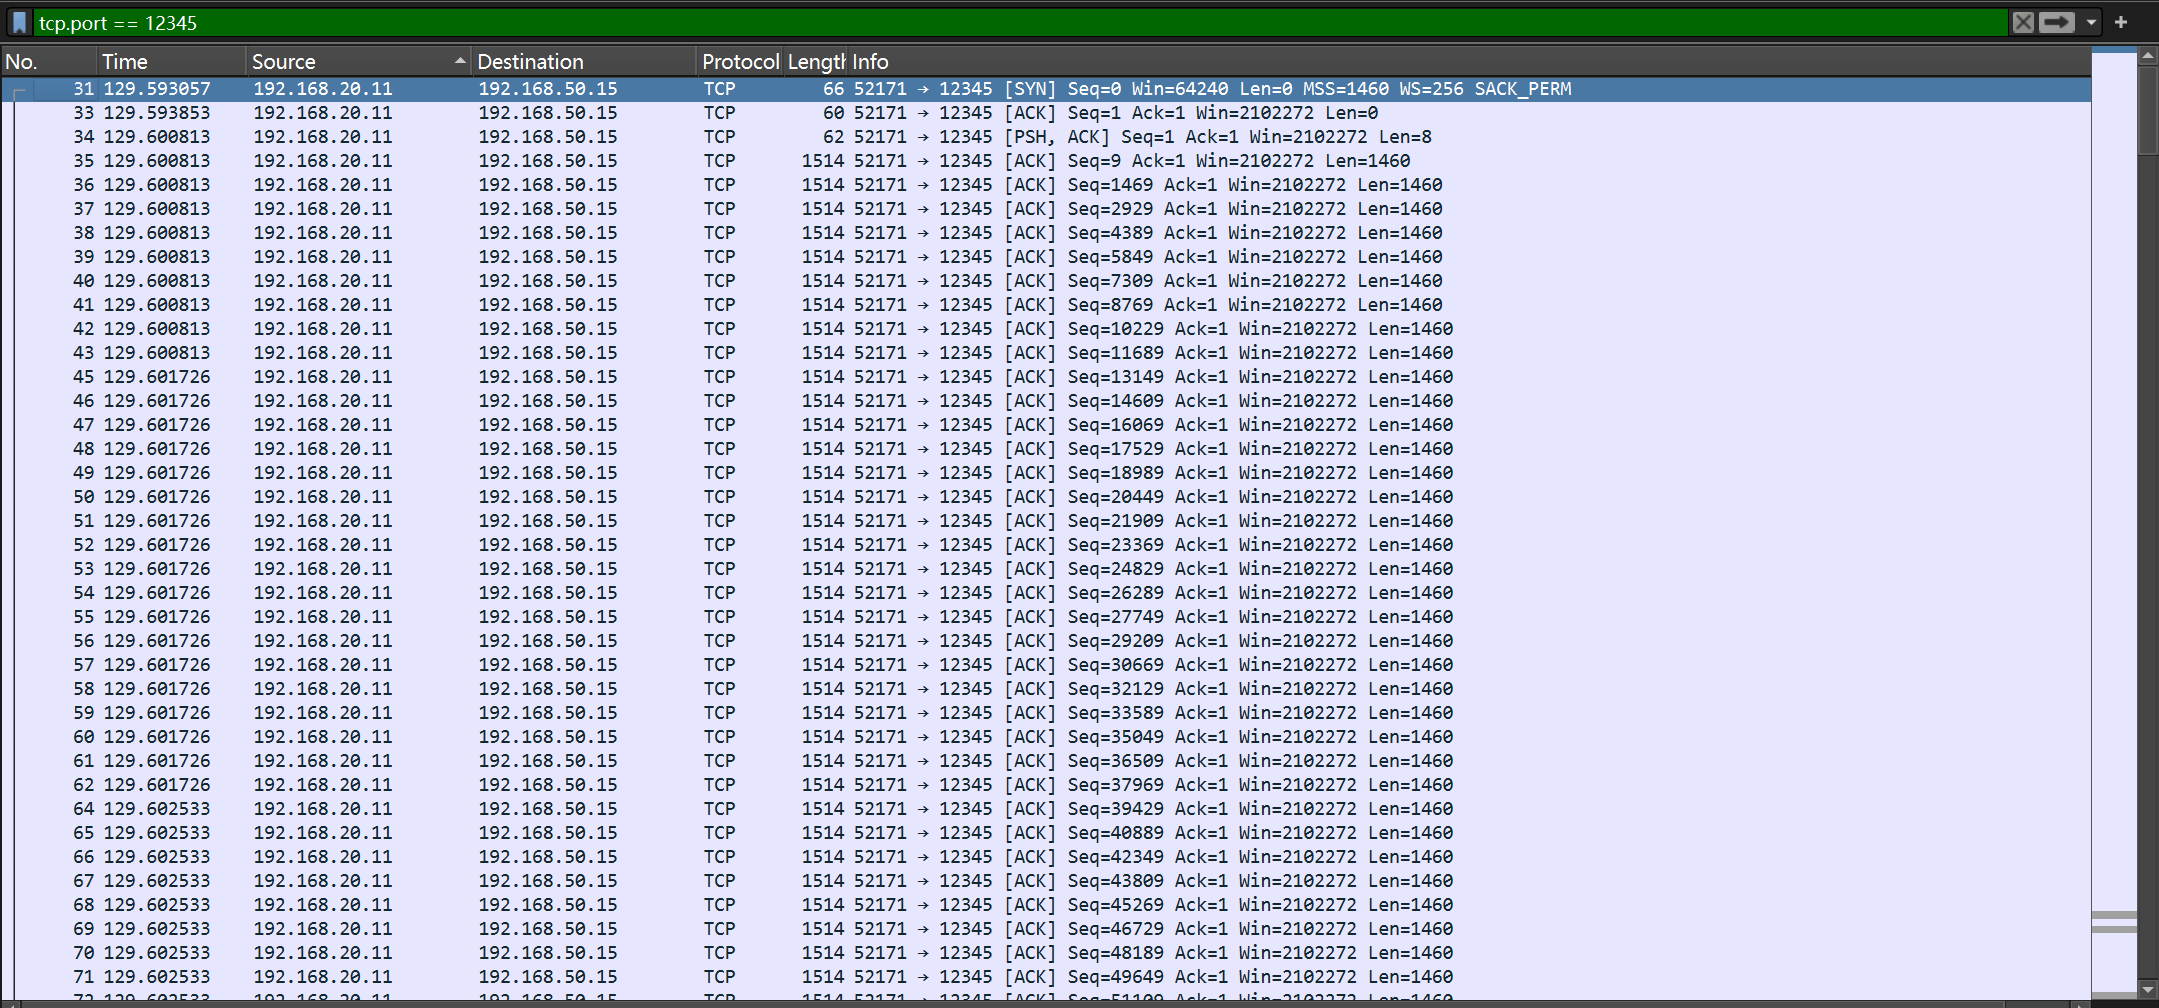
\includegraphics[width=\textwidth]{images/104.png}
    \caption{在H5上捕获的TCP通信全过程。}
\end{figure}
\begin{figure}[H]
    \centering
    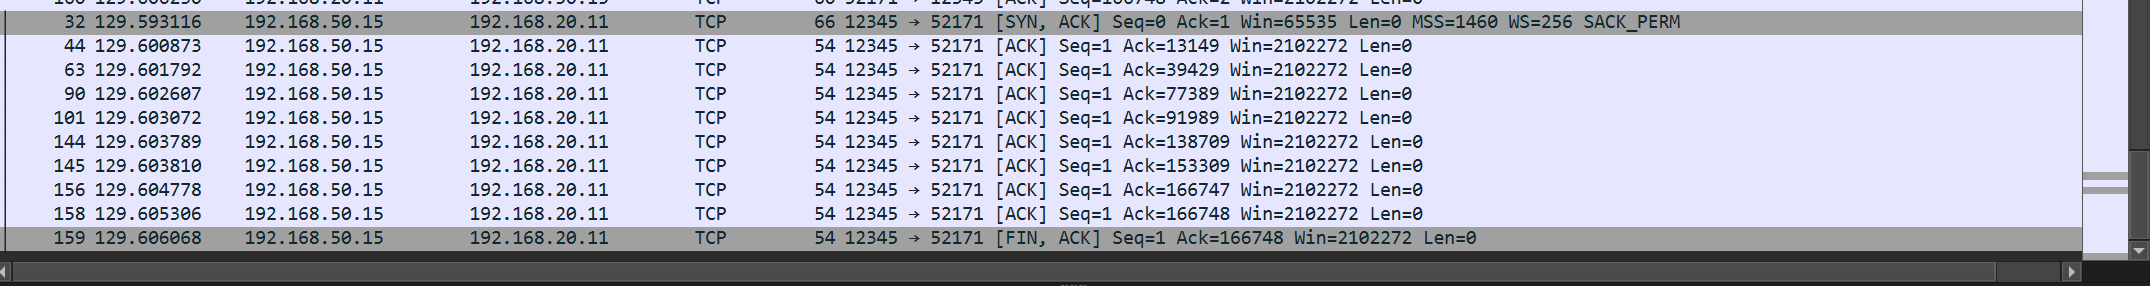
\includegraphics[width=\textwidth]{images/105.png}
    \caption{H5抓包结果的延续部分，显示了完整的ACK和FIN序列。}
\end{figure}

\textbf{关键数据包深度解析 (H5 - 包 35，首个数据段)}
\begin{figure}[H]
    \centering
    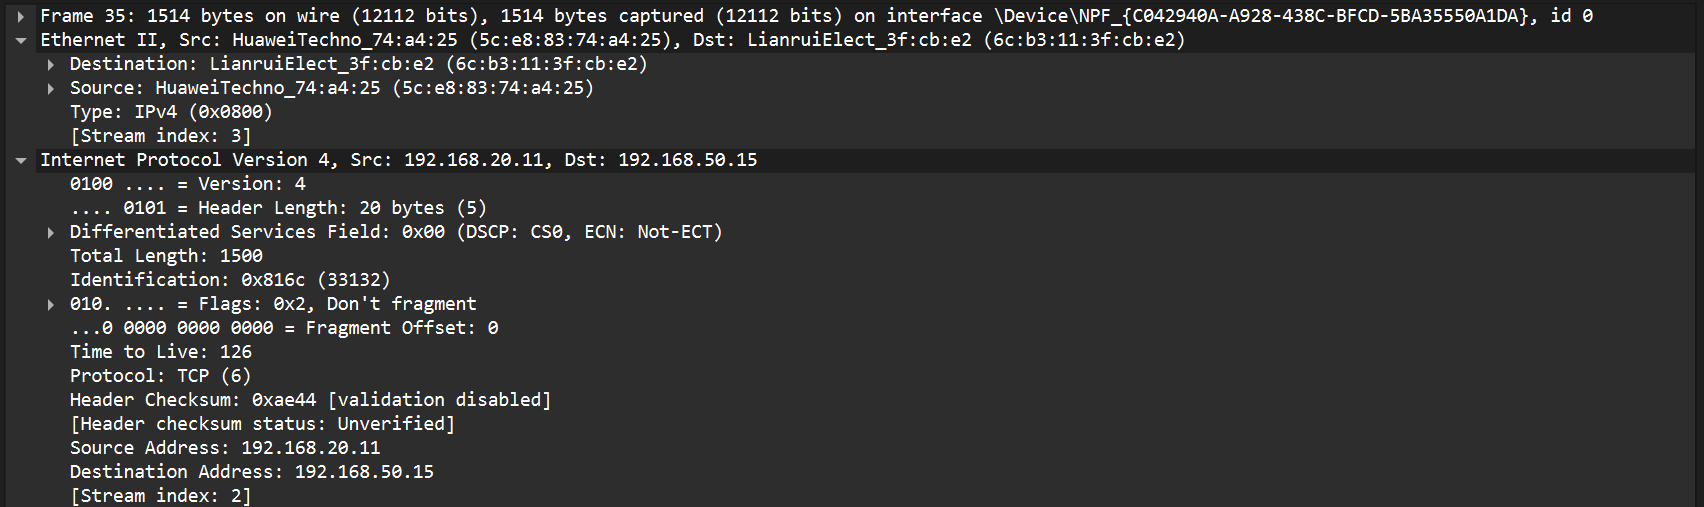
\includegraphics[width=\textwidth]{images/106.png}
    \caption{H5捕获的数据包二层和三层头部。}
\end{figure}
\begin{figure}[H]
    \centering
    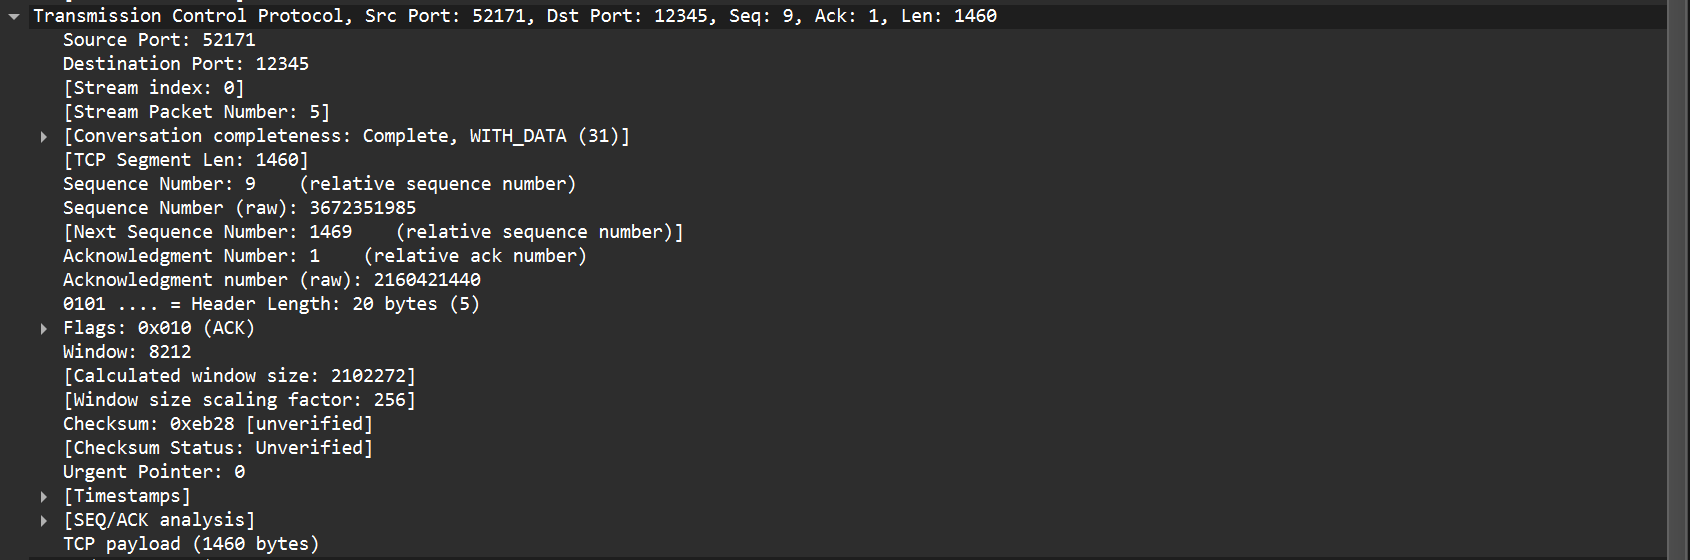
\includegraphics[width=\textwidth]{images/107.png}
    \caption{H5捕获的数据包传输层头部。}
\end{figure}

\textbf{分析}：这是数据包在旅程终点的最后状态。

\begin{itemize}
    \item \textbf{以太网层 (L2)}:
    \begin{itemize}
        \item \textbf{源MAC地址}: \texttt{5c:e8:83:74:a4:25}，即\textbf{路由器R2的出接口(GE0/0/5)的MAC地址}。
        \item \textbf{目的MAC地址}: \texttt{6c:b3:11:3f:cb:e2}，即\textbf{主机H5的网卡物理地址}。MAC地址对再次为当前链路（R2到H5）定制。
    \end{itemize}
    \item \textbf{IPv4层 (L3)}:
    \begin{itemize}
        \item \textbf{IP地址}依旧保持端到端的\texttt{192.168.20.11} $\rightarrow$ \texttt{192.168.50.15}。
        \item \textbf{TTL}变为\texttt{126}。在R2收到的127基础上\textbf{再次减1}，因为数据包又成功穿越了R2。\texttt{128 $\rightarrow$ 127 (经R1) $\rightarrow$ 126 (经R2)}，路径清晰，与\texttt{ping}测试结果完全吻合。
    \end{itemize}
\end{itemize}

总结

本次任务通过编程实践与多点抓包分析，系统性地验证了TCP/IP协议栈在复杂网络环境下的工作机制。

我们的结论如下：

1. \textbf{TCP协议的可靠性}：尽管在中间路由器上观察到了真实的TCP重传现象，但最终接收端H5收到的数据（无论是文字还是图片）与发送端完全一致。这生动地展示了TCP通过序列号、确认和超时重传机制来对抗网络延迟与丢包，从而为上层应用提供可靠的数据流服务。

2. \textbf{交换与路由的本质差异}：
    \begin{itemize}
        \item \textbf{交换}是逐跳的二层操作。交换机在同一广播域内基于MAC地址转发数据帧，此过程对IP包完全透明，不修改任何三层或更高层的头部信息，包括TTL。
        \item \textbf{路由}是 端到端 的三层决策与逐跳的二层重封装的结合。IP地址在全程保持不变，指导着数据包的最终方向。而每经过一个路由器，TTL值减1，并且整个数据链路层帧头被重写，以适应下一跳的物理链路。
    \end{itemize}

3. \textbf{对网络关键字段的理解}：
    \begin{itemize}
        \item \textbf{MAC地址}是链路本地的，用于在单一网段内寻址。
        \item \textbf{IP地址}是全局唯一的，用于在整个互联网中寻址。
        \item \textbf{TTL}是IP包的“生命计数器”，由路由器递减，用以防止数据包在网络中无限循环。
        \item \textbf{TCP序列号/确认号}是保证数据有序、不重、不丢的关键，是TCP可靠性的基石。
    \end{itemize}

\newpage
\section{实验总结}

本次综合实验系统地覆盖了网络工程中的关键技术环节。通过完成五个递进的任务，我们具体实施并掌握了以下内容：

\begin{itemize}
    \item \textbf{任务一：RSTP网络环路防护}
    \begin{itemize}
        \item \textbf{实施：} 在两台交换机之间连接冗余物理链路，并通过启用快速生成树协议（RSTP）解决了由此引发的广播风暴问题。
        \item 掌握了RSTP在二层网络中的作用，理解了其通过逻辑阻塞冗余端口来防止环路、同时保持链路备份的原理。
    \end{itemize}

    \item \textbf{任务二：VLAN划分与VLAN间路由}
    \begin{itemize}
        \item \textbf{内容：} 创建VLAN 10和VLAN 20，配置交换机端口为Access和Trunk模式，并在路由器R1上通过配置子接口和物理接口作为网关，实现了不同VLAN间的通信。
        \item 理解了VLAN如何实现网络逻辑隔离，掌握了Access和Trunk端口的应用场景，并学会了利用三层设备（路由器）作为网关实现VLAN间路由。
    \end{itemize}

    \item \textbf{任务三：OSPF动态路由}
    \begin{itemize}
        \item \textbf{内容：} 在路由器R1和R2之间配置OSPF协议，宣告各自的直连网段，使两台路由器自动学习全网路由。
        \item 掌握了OSPF的基本配置方法，理解了动态路由协议如何自动建立邻居关系、交换路由信息并最终实现全网动态收敛，替代了繁琐的静态路由配置。
    \end{itemize}

    \item \textbf{任务四：基于时间的访问控制列表（ACL）}
    \begin{itemize}
        \item \textbf{内容：} 在R1上定义了不同时间段（\texttt{time-range}），并编写了一套包含\texttt{permit}和\texttt{deny}规则的高级ACL，将其应用于接口以实现分时段的精细化访问控制。
        \item 掌握了使用ACL进行流量过滤的方法，理解了ACL规则自顶向下匹配的顺序重要性，并学会了如何结合时间范围实现复杂的动态安全策略。
    \end{itemize}

    \item \textbf{任务五：TCP编程与全路径抓包分析}
    \begin{itemize}
        \item \textbf{内容：} 编写Python TCP套接字程序实现H1到H5的文件和文本传输。同时，在S1、S2、R1、R2上配置端口镜像，捕获了数据包在完整路径上的传输过程。
        \item 通过抓包分析，直观地验证了网络分层模型的核心原理：
        \begin{itemize}
            \item \textbf{二层交换：} 交换机转发数据帧时不修改IP包内容，TTL值不变。
            \item \textbf{三层路由：} 路由器每转发一次IP包，TTL值减1，并重写数据链路层的MAC帧头以适应下一跳链路。
            \item \textbf{端到端地址：} 在整个传输过程中，源/目的IP地址保持不变，而源/目的MAC地址在每一跳路由后都会改变。
            \item \textbf{TCP可靠性：} 验证了TCP协议确保了数据在跨网络传输后的完整性。
        \end{itemize}
    \end{itemize}
\end{itemize}

\end{document}